% part4.tex

\part{\LaTeX{}浮动图形环境}

\section{浮动图形环境}\label{sec:floatfigure}
在使用字处理软件排版时,用户放在哪里图形就会出现在哪里\footnote{
	尽管许多字处理软件确实可以允许图形在文本周围移动(或者文本在图形周围移动),
	但是出于糟糕的软件设计以及/或者文档作者的忽略,绝大部分用户并不使用该功能。}。
但是,因为这些图形不能被分割开来,所以经常会导致糟糕的分页,将大片的空白留在页面下方。
为得到专家级的排版效果,作者不得不手工调整图形的位置。
这种工作是非常乏味的,尤其是几乎每次修改文档都得这样做一次。

为此,\LaTeX{}~提供了一个浮动图形机制来自动将图形放置到看起来合适的位置,
既能得到专家级的排版效果,又不必手工做调整图形位置的乏味的工作。
不过,它也会给那些习惯于手工调整图形的新手带来不适。
想要有效的利用浮动图形机制需要注意以下几点:
\begin{description}
	\item[不要使用依赖于图形放置位置的文本]
	
	使用如“\emph{这幅图...}”或“\emph{下面的图形...}”等短语要求所指的图形需在固定位置。
	而像~``\emph{图~5...}''~这样的短语则允许图形出现在任意位置。
	\item [放松]
	
	一些用户在发现图形没有十分准确的出现在他们所想要的位置时,往往非常着急。
	这没有必要,图形的放置是 \LaTeX{} 的工作,最好放松一些。
\end{description}

在接下来的几页中我们将介绍 \LaTeX{} 是以怎样的专业级的排版规则来决定浮动图形的位置的。
\marginpar{经验总结}
为方便起见,下面列出关于浮动图形放置的一些最常见问题的解决方法。
\begin{enumerate}
	\item 不要束缚 \LaTeX{} 的手脚。
	给出的浮动选项越多,\LaTeX{} 做的就越好。
	特别地,使用选项 \opt{[htbp]} 和 \opt{[tbp]}	就很好。
	见第~\ref{ssec:figplacement}~节。
	
	\item 很多人发现缺省的浮动参数过于严格了。下面的命令
\begin{lstlisting}
\setcounter{topnumber}{4}
\setcounter{bottomnumber}{4}
\setcounter{totalnumber}{10}
\renewcommand{\textfraction}{0.15}
\renewcommand{\topfraction}{0.85}
\renewcommand{\bottomfraction}{0.70}
\renewcommand{\floatpagefraction}{0.66}
\end{lstlisting}
	将浮动参数重新设置为更宽松的值。详见第~\ref{sec:typerule}~节。
	
	\item \LaTeX{} 允许图形浮动到当前页的顶部,
	这样会使图形在引述它的文本前出现。
	不喜欢这样做的用户可以使用~\pkgi{flafter} 宏包。
	无需使用特殊的命令,只要简单地调入该宏包 \cmdM{usepackage}{flafter} 即可。
	
	\item 要确保图形的浮动不超过某一特定点,
	可调入 \pkgi{placeins} 宏包并使用 \cmdi{FloatBarrier} 命令。见第~\ref{ssec:unprocessfig}~节。
	
	\textbf{警告}:过多使用 \cmd{FloatBarrier}	命令会导致浮动位置难以控制或浮动参数不正确。
	这两种情况都是应当尽量避免的。
\end{enumerate}

\subsection{创建浮动图形}\label{ssec:createfloatfig}
可以通过把命令置于一个 \envi{figure} 环境中来生成浮动图形。
在图形环境中的所有内容都会被保持在一起,
浮动到合适的位置以保证得到最好的分页结果。
另外,可以通过使用 \cmdi{caption} 命令来为浮动图形自动编号并加上标题。
例如,下面的命令将 \file{graph.eps} 中的图像放到一个浮动图形中。
\begin{lstlisting}
\begin{figure} 
\centering 
\includegraphics[totalheight=2in]{graph.eps} 
\caption{一幅插入的EPS图像} \label{fig:graph} 
\end{figure}

第~\pageref{fig:graph} 页的图~\ref{fig:graph}...
\end{lstlisting}

对于图形环境,应当注意:
\begin{itemize}
	\item 可选的 \cmdi{label} 命令和 \cmdi{ref}、\cmdi{pageref} 命令配合使用,
	可对图形标题进行交叉引用。更多信息参见第~\ref{sssec:refcmd} 节。
	\cmd{label} 命令必须紧接着 \cmd{caption} 命令给出。
	如果放在之前的话,那么 \cmd{ref} 会引用上一个可引用对象(通常是所在章节或者是之前的图形)。
	
	\item 如果 \env{figure} 图形环境中没有使用 \cmd{caption} 命令,
	那么就是一个没有编号的浮动图形。
	
	\item 如果一图形环境中使用了多个 \cmd{caption} 命令,
	那么它将生成多个一起浮动的图形。
	这在排版并列放置的图形(见第~\ref{sec:sidebyside} 节)
	或者复杂排列的图形(见第~\ref{sec:stackfigs} 节)时是非常有用的。
	
	\item 可用命令~\cmdi{listoffigures}~来得到一个图形目录。
	\item 缺省地,\cmd{caption} 的文本就是标题内容,也会在图形目录中列出。
	\cmd{caption} 命令的可选项可用来将与标题文本不同的内容加到图形目录中。如:
\begin{lstlisting}
\caption[List Text]{Caption Text}
\end{lstlisting}
	会在标题中使用 \texttt{Caption Text} 而在图形目录中使用 \texttt{List Text}。
	这在使用了特别长的标题时会很有用。
	
	\item \env{figure} 图形环境只能用于段落外模式,不能在段落中使用。
	因此不能放在任何的盒子中(例如 \cmd{parbox} 或 \env{minipage})。
	
	\item 若 \env{figure} 图形环境被置于正文段落中,例如
\begin{lstlisting}
....text text text text text text 
\begin{figure} 
.... 
\end{figure} 
text text text text text text...      
\end{lstlisting}
	那么它在该正文段落结束之前不会被处理。
\end{itemize}

\subsubsection{定义引用命令}\label{sssec:refcmd}
相比于直接输入
\begin{lstlisting}
第~\pageref{fig:graph} 页的图~\ref{fig:graph}
\end{lstlisting}
更为方便的做法是在文档的导言区定义如下命令
\begin{lstlisting}
\newcommand\Figpage[1]{第~\pageref*{#1} 页的图~\ref*{#1}}
\end{lstlisting}
然后引用代码就可以用 \cmdM{Figpage}{fig:graph} 来简化。

\paragraph{条件引用}
以上定义的 \cmd{Figpage} 命令总是会打印出图形编号和页码。
当图形和引用出现在同一页时,通常需要省略页码。
使用如下代码即可
\begin{lstlisting}
\newcommand\FigDiff[1]{第~\pageref{fig:graph} 页的图~\ref{fig:graph}}
\newcommand\FigSame[1]{图~\ref{fig:graph}}
\newcommand\Figref[1]{\ifthenelse{\value{page}=\pageref{#1}}
	{\FigSame{#1}}{\FigDiff{#1}}}
\end{lstlisting}
如果引用和图形在同一页,那么 \cmd{Figref} 命令会调用 \cmd{FigSame} 命令进而显示“图~17”字样。
如果不在同一页,那么 \cmd{Figref} 命令会调用 \cmd{FigDiff} 命令进而显示“第~25页的图~17”字样。

宏包 \pkgi{varioref} \cite{varioref-doc} 还为引用图表、章节等提供了类似的命令。

\subsubsection{hyperref 宏包}\label{sssec:hyperref}

\pkgi{hyperref} 宏包允许用户为 \LaTeX{} 文档创建超链接,
主要结合 \prgname{pdflatex} 一起使用。

\pkg{hyperref} 的特性之一就是重定义了 \cmd{ref} 和 \cmd{cite} 命令,
这样可以作为指向引用的超链接排版显示。
同时,\cmd{ref*} 和 \cmd{cite*} 定义为不含超链接的引用。

由于 \pkg{hyperref} 重定义了很多 \LaTeX{} 命令,
通常用户需要注意 \cmd{usepackage} 的顺序以使得最后导入 \pkg{hyperref} 宏包。
更多信息请参考 \cite{hyperref-doc}。

\paragraph{超文本引用}
当使用 \pkg{hyperref} 宏包时,\cmd{ref} 命令会打印出的图形编号会带有指向该图形的超链接。
由于图形编号数字相对较小,会给点击超链接带来困难,
因此,如下定义的命令会让点击超链接更加容易
\begin{lstlisting}
\newcommand\Figlink[1]{%
	\hyperref[#1]{第~\pageref{fig:graph} 页的图~\ref{fig:graph}}
\end{lstlisting}
使用 \cmd{Figlink} 命令会将“图~17”这样的引用整个地放在超链接里面。


\subsection{图形的放置}\label{ssec:figplacement}

利用 \env{figure} 环境的可选参数项可以指定图形有可能放置的位置。
这一可选参数项可以是下列字母的任意组合。
\begin{description}
	\item [h] \emph{当前位置。} 
	将图形放置在正文文本中给出该图形环境的地方。
	如果本页所剩的页面不够,这一参数将不起作用。
	\item [t] \emph{顶部。} 将图形放置在页面的顶部。
	\item [b] \emph{底部。} 将图形放置在页面的底部
	\footnote{当一幅图形被放置在页面的底部时,
		如果此页有脚注的话,它将位于所有脚注的下方。
		现在还没有办法来避免这种情况。}。
	\item [p] \emph{浮动页。} 将图形放置在允许有浮动体的页面上。
\end{description}

几个注记:
\begin{itemize}
	\item 如果在图形环境中没有给出上述任一参数,则缺省为 \opt{[tbp]}。
	该默认选项可以通过重定义内部命令 \verb|\fps@figure| 定制。
	例如,
\begin{lstlisting}
\makeatletter
\def\fps@figure{htbp}
\makeatother
\end{lstlisting}
	会将缺省值设为 \opt{[htbp]}。
	
	\item 位置参数的顺序不会影响到最后的结果。
	因为 \LaTeX{} 总是尝试以 \texttt{h-t-b-p} 的顺序来确定图形的位置。
	所以 \opt{[hb]} 和 \opt{[bh]} 都会以 \texttt{h-b}	的顺序来排版。
	
	\item 给出的参数越多,\LaTeX{} 的排版结果就会越好。
	一般来说,\opt{[htbp]}、\opt{[tbp]}、\opt{[htp]}、\opt{[tp]} 这些组合得到的效果就很不错。
	
	\item 只给出单个的参数项 \opt{[t]}、\opt{[b]}、\opt{[p]}、\opt{[h]} 极易引发问题
	\footnote{实际上,永远不要单独使用 \opt{[h]} 选项。
		由于使用单个的 \opt{[h]} 选项效果过于糟糕,
		较新版本的 \LaTeX{} 自动将其改为 \opt{[ht]}。}。
	如果该图形不适合所指定的位置,它就会被搁置并阻碍对接下来图形的处理。
	一旦这些阻塞的图形数目超过了18幅这一 \LaTeX{} 所能容许的最大值,
	就会产生 ``Too Many Unprocessed Floats'' 的错误(见第~\ref{ssec:toomanyfig}~节)。
\end{itemize}

当 \LaTeX{}“\emph{试图}”放置一浮动图形时,
\marginpar{见 \cite[第~198~页]{Lamport1994}}
它将遵循以下规则:
\begin{enumerate}
	\item 图形只能置于由位置参数所确定的地点。
	\item 图形的放置不能造成页面溢出(\texttt{overfull page})。
	\item 图形只能置于当前页或后面的页中
		\footnote{因为图形可浮动到当前页的顶部,所以它可能会出现在它所在文本的前面。
			如果要防止出现这种情况,可使用 \pkg{flafter}宏包。
			只要使用 \cmd{usepackage} 导入宏包即可,
			不需要使用什么命令。}。
	所以图形只能“向后浮动”而不能“向前浮动”。
	\item 图形必须按顺序出现。当前图形只有当之前的图形都被放置好之后才能被放置。
	进一步又有两个衍生规则:
	\begin{itemize}
		\item 只要前面有未被处理的图形,一幅图形就不会被放在当前位置。
		\item 一幅“不可能放置”的图形将阻碍它后面的图形的放置。
		直到文件结束或达到~\LaTeX{}~的浮动限制。参见第~\ref{ssec:toomanyfig}~节。
	\end{itemize}
	同样地,一表格也只能在其前面的表格都被处理完后才能被放置。
	不过,表格在排版时是跳过图形而单独处理的。
	反之,图形的处理也是与表格的处理无关的。
	\item 必须符合在第~\ref{sec:typerule}~节中给出的审美条件。
	例如,一页上的浮动体的数目不能超过 \opt{totalnumber}\index{totalnumber@\texttt}。
	在浮动位置选项前加上一个惊叹号(如 \cmdM{begin}{figure}\opt{[!ht]})
	会使 \LaTeX{} 忽略应用于文本页的审美条件,试图强制放置浮动图形。
	不过,\texttt{!} 不会影响应用于浮动页的审美条件。
\end{enumerate}


\subsection{清除未处理的浮动图形}\label{ssec:unprocessfig}

使用浮动体的一大优势就是不需要将它们立即放置在输入它们的地方。
\LaTeX{} 会将它们暂时保存,直到在更合适的地点加以放置。
当一浮动图形已被~\LaTeX{}~读入,但还没有将它放到页面上时,
这一图形被称为“未处理浮动图形”。
虽然 \LaTeX{} 处理浮动体的算法通常很好,
但有时还是需要手动强制处理那些未处理的浮动图形。

下面的三个方法都可以用来清除未处理的浮动图形。
这些命令必须分开使用。
然而,过度使用这些方法要么说明手动管理浮动体位置过去细致,
要么说明位置参数有问题(见第~\ref{sec:typerule}~节)。

\begin{description}
	\item [clearpage] \mbox{} \\
	最基本的用来清除未处理的浮动图形的方法就是使用 \cmdi{clearpage} 命令。
	它可让 \LaTeX{} 排版所有未处理的浮动图形并开始一新页。
	尽管这一命令很有效,但它也常常导致页面的下方出现很大的空白。
	
	\item [FloatBarrier] \mbox{} \\
	对于大多数情况,最好的方法是使用 \pkgi{placeins} 宏包提供的 \cmdi{FloatBarrier} 命令。
	使用 \pkg{placeins} 宏包有三种方法:
	\begin{enumerate}
		\item \cmd{FloatBarrier} 使所有未处理的浮动图形立即被处理。
		但与 \cmd{clearpage} 不同的是,它不会开始一新页。
		\item 很普遍的一种情况是要求浮动图形在它们所在的章节中排出,
		为此可在调用 \pkg{placeins} 宏包时使用 \opt{section} 选项:
\begin{lstlisting}
\usepackage[section]{placeins}
\end{lstlisting}
		这样会重新定义 \cmd{section} 命令,
		在每一节之前都加上一个 \cmd{FloatBarrier} 命令。
		
		注意这个 \opt{[section]} 选项是很严的。
		举例来说,如果在一页的中间开始新的一节,
		那么上面这个 \opt{section} 选项会阻止上一节的浮动图形放置在这一页的底部,
		因为这样会在新的一节之后。
		\item 使用 \opt{below} 选项:
\begin{lstlisting}
\usepackage[below]{placeins}
\end{lstlisting}
		会比使用 \opt{section} 选项松一些。
		它允许上一节的浮动图形出现在新一节之后,只要在同一页中有上一节的内容。
	\end{enumerate}
	\pkg{placeins} 宏包不会改变浮动体的顺序。
	例如,由于 \cmd{FloatBarrier} 只能在当前页的顶部放置带 \opt{[t]} 选项的浮动体,
	因此,\cmd{FloatBarrier} 命令处理时会在当前页留白并另起新一页,
	然后将带 \opt{[t]} 选项的浮动体放置在新一页的顶端。
	类似地,\cmd{FloatBarrier} 不能在当前位置放置带 \opt{[b]} 选项的浮动体,
	因此会禁止文本出现在该浮动体的下面。
	
	这两个例子再次说明了,
	当指定多个位置选项(例如 \opt{[tbp] 或 \opt{[htbp]}})时,
	浮动体位置的处理方式会更加有效。

	\item [afterpage/clearpage] \mbox{} \\
	\pkgi{afterpage} 宏包提供了命令 \cmdi{afterpage},
	可以在下一自然分页时执行一个命令。
	因此,用
\begin{lstlisting}
\afterpage{\clearpage}
\end{lstlisting}
	会使所有未处理的浮动体在下一分页前被清除完。
	
	使用 \cmdM{afterpage}{\cmd{clearpage}} 并不总可以解决浮动限制问题
	(见第~\ref{ssec:toomanyfig}~节)。
	因为它只是在页面结束前才会执行 \cmd{clearpage} 命令,
	而到页面结束时可能又会累积新的未处理的浮动体,
	进而可能已超过了 \LaTeX{} 的限制。
	
	\cmdM{afterpage}{\cmd{clearpage}} 命令在排版尺寸较小的浮动页图形时特别有用。
	而命令 \cmd{floatpagefraction} (见第~\ref{ssec:figpara} 节)
	会阻止“太小”的图形在浮动页上出现。
	此外,由于浮动位置标识符 \texttt{!} 不会应用于浮动页,
	因此 \opt{[!p]} 不会破除 \cmd{floatpagefraction} 的限制,
	使用 \cmdM{afterpage}{\cmd{clearpage}} 既可以克服 \cmd{floatpagefraction} 的限制,
	又不会导致正文页有较多空白。
\end{description}


\subsection{过多未处理的浮动体}\label{ssec:toomanyfig}

如果一浮动体不能被即时处理,它就会被放到未处理的浮动体队列中等待处理。
由于这一队列只能有 18 个位置,
所以当未处理的浮动体的数目超过这一限制时就会导致发生“Too Many Unprocessed Floats”的错误。
造成这种错误有四种可能的原因:

\begin{enumerate}
	\item 最常见的原因是浮动位置选项与浮动位置参数冲突。
	例如对于一个带 \opt{[t]} 选项的 \env{figure} 环境,
	如果它的高度超过了 \cmd{topfraction} 的值,就会被放到等待处理队列中。
	其它单位置选项也有类似的问题,
	所以给出尽可能多的浮动位置选项。

	\item 不适当的浮动体比例参数值会造成一些图形无法放置。
	要防止出现这种情况,一定要确保所使用的比例参数值满足第~\ref{ssec:figpara} 节中对此的要求。

	\item 在很少的情况下,如使用了很多浮动体和 \cmd{marginpar} 边注
	(会和浮动体使用相同的未处理队列机制相同),
	可能确实需要较长的等待队列。
	这时可使用 \pkgi{morefloats} 宏包将等待队列的长度限制增加到 36。

	\item 如果超过18幅图形在之间没有任何文本的情况下被读入,
	就会超出 \LaTeX{} 浮动放置队列的最大数目。可能的解决办法有:
	
	\begin{enumerate}
		\item 将图形散布在正文中。
		这会使得有足够的文本来自然分页,\LaTeX{} 也会更容易地处理浮动体。
		\item 在这些图形之间加入 \cmd{clearpage}。
		这样做可能得花费一些时间来调整页面以避免产生有很大空白的页。
		注意,尽管 \cmdM{afterpage}{\cmd{clearpage}} 会在下一个自然分页处调用 \cmd{clearpage},
		但在此情况下并不起作用,
		因为引发自然分页需要足够的文本,在这之前就会超过浮动体队列限制了。
		\item 因为这里没有文本,所以图形并不需要浮动。
		因此,最好的解决办法也许是采用第~\ref{sec:nonfloat}~节中的方法来构建非浮动的图形,
		同时用 \cmd{vspace} 和 \cmd{vfill} 来提供竖直间距。
	\end{enumerate}
\end{enumerate}


\section{定制浮动位置}\label{sec:typerule}

下列的样式参数用于避免页面生成糟糕的浮动体效果,
例如一页中的浮动体数量过多或者位置错误。
如果在正文中的某处修改这些参数,那么直到下一页才会生效。
不过,如果是在导言区修改的话,就会对整个文档都起作用。

\subsection{浮动位置的计数器}

表~\ref{tab:floatcounter} 中所给出的三个计数器可用于防止 \LaTeX{} 将过多的浮动体置于同一文本页中,
但它们不会影响浮动页。
在浮动位置选项前加上 \texttt{!} 会让 \LaTeX{} 忽略这些计数器。
这些计数器的值可用 \cmdi{setcounter} 命令来设置。例如:
\begin{lstlisting}
\setcounter{totalnumber}{2}
\end{lstlisting}
会阻止 \LaTeX{} 将多于两个的浮动体放置到一文本页中。
许多人感觉默认的浮动位置计数器太严格了,更喜欢宽松一些的设置,例如
\begin{lstlisting}
\setcounter{topnumber}{4}
\setcounter{bottomnumber}{4}
\setcounter{totalnumber}{10}
\end{lstlisting}

\begin{table}[htp]
	\centering\kaishu
	\caption{浮动位置计数器}\label{tab:floatcounter}
	\begin{tabular}{>{\ttfamily}l p{0.7\textwidth} }
		\toprule
		topnumber & 可以位于文本页顶部的浮动体的最大数目(缺省值为 2)。\\
		\hline
		bottomnumber & 可以位于文本页底部的浮动体的最大数目(缺省值为 1)。\\
		\hline
		totalnumber & 可以位于文本页中的浮动体的最大数目(缺省值为 3)。 \\
		\bottomrule
	\end{tabular}
\end{table}

\subsection{图形环境中的比例参数}\label{ssec:figpara}

表 \ref{tab:floatfraction} 中给出的命令用来控制一页中有多大比例的区域可用来放置浮动体
(这里的比例是指浮动体的高度除以正文高度 \cmd{textheight})。
前面三个命令只作用于文本页,
而最后一个命令只作用于浮动页。
在浮动位置选项前加上 \texttt{!} 会让 \LaTeX{} 忽略前面三个命令,
而 \cmdi{floatpagefraction} 总是起作用的。
这些命令的值可以用 \cmd{renewcommand} 来修改。例如:
\begin{lstlisting}
\renewcommand{\textfraction}{0.3}
\end{lstlisting}
限定浮动体不得超过文本页的 $70\percent$。

\begin{table}[hbp]
	\centering\kaishu
	\caption{图形位置的比例参数}\label{tab:floatfraction}
	\begin{tabular}{ l p{0.65\textwidth}}
		\toprule
		\cmd{textfraction} & 页面中必须用于文本的最小比例。缺省值为 0.2,
		即一页中浮动体所占的比例不得超过 $80\percent$。 \\
		\hline
		\cmd{topfraction} &  文本页中页面顶部可以用来放置浮动体的最大空间比例。
		缺省值为~0.7,即放置在顶部的浮动体所占的高度不得超过整个页面高度 $70\percent$。
		同样地,如果多个使用了选项 \opt{t} 的浮动体的高度和超过了整个页面高度的 $70\percent$,
		即使它们的数目没有超过 \texttt{topnumber} 的值,
		仍将一个也不会被放置在页面顶部。 \\
		\hline
		\cmd{bottomfraction} & 文本页中页面底部可以用来放置浮动体的最大空间比例。
		缺省值为~0.3,即,
		只有当浮动体的高度不超过整个页面高度的 $30\percent$ 时才可以放置在页面底部。\\
		\cline{2-2}
		\cmd{floatpagefraction} & 浮动页中必须由浮动体占用高度的最小比例。
		因此在浮动页中空白所占的比例不会超过~$1-\text{\cmd{floatpagefraction}}$。
		缺省值为~0.5。\\
		\bottomrule
	\end{tabular}
\end{table}

这些默认的位置比例参数值既
\marginpar{比例系数使用指引}
可以防止过多/过大的浮动体占据文本页面的主要空间,
也可以防止在浮动页上有很大的空白而只有很小的图形。
虽然这些缺省值让 \LaTeX{} 运作得很好,但有时显得稍稍严了些,
结果导致有些浮动体到标明它们的命令距离很远。
这种情况下,可以将这些比例的值放宽松些,例如:
\begin{lstlisting}
\renewcommand{\textfraction}{0.15} 
\renewcommand{\topfraction}{0.85} 
\renewcommand{\bottomfraction}{0.70} 
\renewcommand{\floatpagefraction}{0.66}
\end{lstlisting}

在调整这些比例值的时候必须要小心,不适当的比例值会导致糟糕的排版结果或者大量未处理的浮动体。
要避免出现这类问题,应该基于如下的一些原则:
\begin{description}
	\item [\cmd{textfraction}] \mbox{} \\
	不要让 \cmd{textfraction} 的值小于0.15,
	因为这样的文本页难以阅读。
	如果一幅图的高度超过了 \cmd{textwidth} 的 $85\percent$,
	那么最好将它单独放置到一浮动页上。
	这样的效果肯定比勉强将它放置到一文本页,而且下方还有一两行文本的效果好得多。
	
	进一步地,永远不要将 \cmd{textfraction} 的值设为零以便允许文本页中不含文本。
	这样作会让 \LaTeX{} 感到迷惑并导致低劣的排版结果。
	
	\item [\cmd{topfraction}] \mbox{} \\
	不要使~\cmd{topfraction}~的值大于 $1-\text{\cmd{textfraction}}$,
	否则会使 \LaTeX{} 的浮动定位算法发生矛盾\footnote{
		旧译本误作“小于 $1-\text{\cmd{textfraction}}$”。——译注}。
	
	\item [\cmd{bottomfraction}] \mbox{} \\
	好的排版风格不提倡在页面的底部放置太多的图形,
	故 \cmd{bottomfraction} 的值一般要比 \cmd{topfraction} 小。
	不要使 \cmd{bottomfraction} 的值大于 $1-\text{\cmd{textfraction}}$。
	否则会使 \LaTeX{} 的浮动定位算法发生矛盾。
	
	\item [\cmd{floatpagefraction}] \mbox{} \\
	如果 \cmd{floatpagefraction} 的值很小,
	那么每一浮动页上就只能放置一个浮动体。
	当放置的浮动体很小的时候,会使浮动页上出现很大面积的空白。
	
	如果 \cmd{floatpagefraction} 的值大于 \cmd{topfraction} 的值,
	使用 \opt{[tp]} 选项的浮动图形就有可能被阻塞而无法排版。
	例如,假设一个带有 \opt{[tp]} 选项的图形高度大于 \cmd{topfraction} 却小于 \cmd{floatpagefraction},
	那么由于它既无法放置在文本页上,也无法放置在浮动页上,所以就被阻塞而无法处理。
	为避免出现这样无法处理的情况,
	\cmd{topfraction} 和 \cmd{floatpagefraction} 的值必须满足以下的不等式:
	\[
	\text{\cmd{floatpagefraction}} \leq \text{\cmd{topfraction}} - 0.05.
	\]
	后面的 0.05 这一项是由于文本页和浮动页有不同的竖直间距
	\footnote{特别地,当比较图形的高度比例和 \cmd{topfraction} 时,
		\cmd{textfloatsep} 和其它文本页浮动间距都被计算在内。
		而对浮动页来说,在考察图形的高度比例是否超过了 \cmd{floatpagefraction} 时,
		浮动间距是不被计算在内的。
		因此,必须从 \cmd{topfraction} 中减去 \cmd{textfloatsep} 除以 \cmd{textheight} 的值(约为0.05)。关于图形间距详见第~\ref{ssec:vspace}~节。}。
	同样地,如果使用了 \opt{[bp]} 或 \opt{[hbp]},
	那么 \cmd{floatpagefraction} 和 \cmd{bottomfraction} 要满足:
	\[
	\text{\cmd{floatpagefraction}} \leq \text{\cmd{bottomfraction}} - 0.05.
	\]
	注意缺省值并不满足上面的不等式,
	因此在处理带有 \opt{[bp]} 或 \opt{[hbp]} 选项的图形时偶尔可能会有问题。
\end{description}

\subsection{限制浮动}

\cmdi{suppressfloats}~阻止在当前页的顶部或底部出现额外的浮动体。
但是不会影响带有 \opt{h} 或者 \opt{!} 选项的图形位置。

在一幅图形之前给出 \cmd{suppressfloats[t]} 会阻止图形出现在文本中位置的上方。
进一步地,\pkgi{flafter} 宏包重定义了 \LaTeX{} 的浮动算法,可以在整个文档中阻止这种现象。
\begin{table}[hbp]
	\centering
	\caption{Suppressfloats 的选项}\label{tab:suppressfloat}
	
	\begin{tabular}{>{\ttfamily}l p{0.65\textwidth}}
		\toprule
		\cmd{suppressfloats}\opt{[t]} & 阻止当前页的顶部出现其它的浮动体。 \\
		\hline
		\cmd{suppressfloats}\opt{[b]} & 阻止当前页的底部出现其它的浮动体。 \\
		\hline
		\cmd{suppressfloats} & 同时阻止当前页的顶部和底部出现其它的浮动体。 \\
		\bottomrule
	\end{tabular}
\end{table}


\section{定制figure环境}\label{sec:customfigure}

\subsection{图形的间距}\label{ssec:vspace}

表~\ref{tab:figlength-textpage}~中给出的长度控制两幅图形之间或图形与正文的间距。
与其它大部分的~\LaTeX{}~长度不同的是,这三个都是橡皮长度,
这就使得可以通过缩短或拉伸获得更好的排版页面。
这些长度可用 \cmd{setlength} 命令来设定。例如:
\begin{lstlisting}
\setlength{\floatsep}{10pt plus 3pt minus 2pt}
\end{lstlisting}
将 \cmdi{floatsep} 的正常值设定为~10\pt。
此外,为了改善页面排版,浮动体的间距可以从 8\pt 到 13\pt 之间调节。

由于 \LaTeX{} 在每一个按照选项 \opt{h} 排在当前位置的浮动体前后都放置一个 \cmdi{intextsep} 间距,
因此两个连续的带 \opt{h} 选项的浮动体之间的间距是 \cmd{intextsep} 的两倍。
为了消除这一额外间距,可以将两个浮动体合并成一个。
不过这样的话,浮动位置算法就不会分开放置,得到的排版效果没有分开时那么好。

\begin{table}
	\centering
	\caption{文本页面中的浮动图形间距}\label{tab:figlength-textpage}
	\kaishu
	\begin{tabular}{>{\ttfamily}l P{0.7\textwidth}}
		\toprule
		\cmdi{floatsep} & 出现在页面的顶部或底部的浮动体之间的垂直距离。
		缺省为 \texttt{12pt plus 2pt minus 2pt}。 \\
		\hline
		\cmdi{textfloatsep} & 出现在页面的顶部或底部的浮动体与文本之间的垂直距离。
		缺省为~\texttt{20pt plus 2pt minus 4pt}。 \\
		\hline
		\cmdi{intextsep} & 出现在页面中间的浮动体
		(如使用了 \opt{h} 选项的浮动体)与上下方文本之间的垂直距离。
		缺省为~\texttt{12pt plus 2pt minus 2pt}。 \\
		\bottomrule
	\end{tabular}
\end{table}

表~\ref{tab:figlength-textpage}~中给出的长度不会影响浮动页上各浮动体之间的距离。
它们由表~\ref{tab:figlength-floatpage}~中给出的长度控制。
浮动页面中的空白经常使用单位 \texttt{fil},
类似于 \cmdi{vfill} 生成的垂直间距,具有无限伸展的能力。
当在一段距离中出现多个 \texttt{fil} 时,它们将按比例填充这段距离。
例如,默认的浮动页面参数效果是,
浮动页面上的浮动体之间的距离是最顶端浮动体到页面顶端距离的两倍,
也是最底端浮动体到页面底端距离的两倍。

\begin{table}
	\centering
	\caption{浮动页面中的浮动体间距}\label{tab:figlength-floatpage}
	\kaishu
	\begin{tabular}{>{\ttfamily}l P{0.7\textwidth}}
		\toprule
		\cmdi{@fptop} & 浮动页中顶部的浮动体上方的空白。
		缺省为~\texttt{0pt plus 1.0fil}。 \\
		\hline
		\cmdi{@fpsep} & 浮动页中的浮动体之间的距离。
		缺省为~\texttt{8pt plus 2.0fil}。 \\
		\hline
		\cmdi{@fpbot} & 浮动页中底部的浮动体下方的空白。
		缺省为~\texttt{0pt plus 1.0fil}。 \\
		\bottomrule
	\end{tabular}
\end{table}

在表~\ref{tab:figlength-floatpage}~中的长度名字中的 \texttt{@} 表示
这是一个 \LaTeX{} 内部命令\footnote{
	用户所有涉及到 \LaTeX{} 内部命令的代码都必须包含在 \cmd{makeatletter} 和 \cmd{makeatother} 之间。
	为实现它的功能, \LaTeX{} 使用了很多普通用户无需涉及的内部命令。
	为防止这些内部命令名字和用户定义的命令的名字发生冲突,
	\LaTeX{} 在它的内部命令名字前加上了一个\texttt{@}。
	由于 \LaTeX{} 命令的名字只能包含字母,
	所以通常不可能定义一个含有 \texttt{@} 的命令。
	不过,命令~\cmdi{makeatletter} 让 \LaTeX{} 把 \texttt{@} 当作字母,
	从而可以定义带有~\texttt{@} 的命令。
	命令~\cmdi{makeatother} 则重新令 \LaTeX{} 不把 \texttt{@} 当作字母。
	}。
所以,所有改变这些长度的 \cmd{setlength} 命令都必须放到 \cmd{makeatletter}  和 \cmd{makeatother} 之间。例如:
\begin{lstlisting}
\makeatletter 
\addtolength{\@fpsep}{4pt} 
\makeatother
\end{lstlisting}
将浮动页中浮动体之间的距离增加了 4\pt。

\subsection{图形上下方的水平线}\label{ssec:fig-line}

通过重新定义 \cmdi{topfigurerule} 和 \cmdi{bottomfigurerule} 命令可在文本和页面顶部或底部的浮动图形之间画一条水平线。
尽管 \cmd{topfigurerule} 和 \cmd{bottomfigurerule} 是已经定义的 \LaTeX{} 命令,
但是由于它们奇特的定义方式,在重定义时要用 \cmd{newcommand} 而不是 \cmd{renewcommand}。

为了不破坏版面,这些命令所加标尺的高度必须为零。
例如要画一条 $0.4\pt$ 的水平线,就必须加上 $-0.4\pt$ 的距离:
\begin{lstlisting}
\newcommand{\topfigrule}{\hrule\vspace{-0.4pt}}
\end{lstlisting}
因为 \cmd{topfigrule} 在 \cmd{textfloatsep} 之前被执行,
上面的命令没有在图形与水平线之间留出距离。
下面的命令则在图形与水平线之间留出了 5\texttt{pt} 的空间。
\begin{lstlisting}
\newcommand{\topfigrule}{% 
	\vspace*{5pt}\hrule\vspace{-5.4pt}} 
\newcommand{\botfigrule}{% 
	\vspace*{-5.4pt}\hrule\vspace{5pt}}
\end{lstlisting}

\begin{table}
	\centering
	\caption{图形标尺命令}\label{tab:figrulecmd}
	\kaishu
	\begin{tabular}{>{\ttfamily}l P{0.7\textwidth}}
		\toprule
		\cmdi{topfigrule} & 该命令在一页顶部的最后一个浮动体后,
		\cmd{textfloatsep} 前被执行的命令(见第~\ref{ssec:vspace}~节)。 \\
		\hline
		\cmdi{bottomfigrule} & 该命令在一页底部第一个浮动体前,
		\cmd{textfloatsep} 后被执行。\\
		\bottomrule
	\end{tabular}
\end{table}

在这里 \cmd{topfigrule} 的定义中,
首先向下移动 $5\pt$ (进入到~\cmd{textfloatsep} 的区域)
以提供图形与水平线之间的距离,然后画上一高为 $0.4\pt$ 的水平线,
最后再向上移动 $5.4pt$ 以补偿前面向下的位移。
同样地,\cmd{botfigrule} 在图形与水平线之间留出了 $5\pt$ 的空间。

由于上面的命令使得图形与水平线之间的距离为 $5\pt$,
所以水平线与文本之间的距离为~$\text{\cmd{textfloatsep}}-5\pt$(见第~\ref{ssec:vspace}~节)。

水平线的厚度缺省为 $0.4\pt$,
并可用 \cmd{hrule} 命令的 \opt{height} 选项来改变。
\begin{lstlisting}
\newcommand{\topfigrule}{% 
	\vspace*{5pt}{\hrule height0.8pt}\vspace{-5.8pt}} 
\newcommand{\botfigrule}{% 
	\vspace*{-5.8pt}{\hrule height0.8pt}\vspace{5pt}}
\end{lstlisting}

\paragraph{需要注意下面几点:}
\begin{itemize}
	\item \cmd{topfigrule} 和 \cmd{botfigrule} 命令对浮动页上的图形
	和放置在当前位置的图形(如使用了\opt{h} 选项)不起作用。
	如果一放置在当前位置的图形正好位于页面的顶部或底部,也不会画上水平线。
	\item 即便图形很宽,水平线的长度也只与文本的宽度相等(参见第~\ref{sec:widefig} 节)。
	\item 因为 \LaTeX{} 的\cmd{rule} 命令在 \cmd{parskip} 不为零时会产生额外的空白,
	所以代之以 \TeX{} 命令 \cmd{hrule}。
\end{itemize}


\subsection{图形与标题的间距}\label{ssec:capspace}

\LaTeX{} 假定图形的标题位于图形的下方,
故而在标题上方保留了更多的空白。因此
\begin{lstlisting}
\begin{figure} 
	\centering 
	\caption{图像上方的标题} 
	\includegraphics[width=2in]{graphic.eps} 
\end{figure}
\end{lstlisting}
生成的图~\ref{fig:verynearcap}~中标题和图形非常接近。

\begin{figure} 
	\centering 
	\caption{图像上方的标题} \label{fig:verynearcap}
	\includegraphics[width=2in]{graphic.eps} 
\end{figure}

标题的垂直间距由长度 \cmdi{abovecaptionskip} 和 \cmdi{belowcaptionskip}
(缺省分别为 10\pt 与零)控制。
可以用标准的 \LaTeX{} 命令 \cmd{setlength} 和 \cmd{addtolength} 来修改。
例如:
\begin{lstlisting}
\begin{figure} 
	\setlength{\abovecaptionskip}{0pt} 
	\setlength{\belowcaptionskip}{10pt} 
	\centering 
	\caption{图像上方的标题} 
	\includegraphics[width=2in]{graphic.eps} 
\end{figure}
\end{lstlisting}
得到图~\ref{fig:normalabovefig}。其中标题的上方没有额外的空白,与图形之间则有 10\pt 的距离。

\begin{figure} 
	\setlength{\abovecaptionskip}{0pt} 
	\setlength{\belowcaptionskip}{10pt} 
	\centering 
	\caption{图像上方的标题}\label{fig:normalabovefig}
	\includegraphics[width=2in]{graphic.eps} 
\end{figure}

如果文档的所有浮动体标题都位于顶部,那么可将如下命令放到导言区:
\begin{lstlisting}
\setlength{\abovecaptionskip}{0pt}
\setlength{\belowcaptionskip}{10pt}
\end{lstlisting}
从而对整个文档都起作用(包括图形和表格)。
如果只是有一部分标题要求位于浮动体的上方,那么可定义如下的命令:
\begin{lstlisting}
\newcommand{\topcaption}{% 
	\setlength{\abovecaptionskip}{0pt}% 
	\setlength{\belowcaptionskip}{10pt}% 
	\caption}
\end{lstlisting}
此时 \cmdM{topcaption}{标题文本} 生成的标题放在浮动体顶部就很合适。

另外还有两种方法可以使浮动体顶部的标题具有合适的间距:
\begin{itemize}
	\item 使用 \pkg{caption} 宏包的 \opt{position=top} 选项
	(见表~\ref{tab:caption-spaceopt})
	可以交换 \cmd{abovecaptionskip} 和 \cmd{belowcaptionskip} 的长度。
	
	\item \pkgi{topcapt} 宏包 \cite{topcapt-doc} 定义了一个 \cmd{topcaption} 命令,
	可以在交换  \cmd{abovecaptionskip} 和 \cmd{belowcaptionskip} 的长度的同时生成标题。
\end{itemize}

\subsection{标题的标记}\label{ssec:captionlabel}

缺省情况下,\LaTeX{} 会在图形的标题开头加上像~``Figure 13: ''~这样的标记。
其中的 ``Figure'' 可以通过重定义 \cmdi{figurename} 来更改。例如,下面的命令
\begin{lstlisting}
\begin{figure} 
	\centering 
	\includegraphics[width=1in]{graphic.eps} 
	\renewcommand{\figurename}{Fig.} 
	\caption{This is the Caption} 
\end{figure}
\end{lstlisting}
得到如图~\ref{fig:figname}~的结果。
至于标题文本的字体,分隔符~``:''~以及其它标题属性的修改可用~\pkg{caption}~宏包
(见第~\ref{sec:caption-pkg}~节)来完成。

\begin{figure} 
	\centering 
	\includegraphics[width=1in]{graphic.eps} 
	\renewcommand{\figurename}{Fig.} 
	\caption{This is the Caption}\label{fig:figname} 
\end{figure}

\subsection{标题的编号}

图形编号的默认方式是使用阿拉伯数字 $1,2,3,\dots$
这可以通过重新定义 \cmdi{thefigure} 命令来改变。

当前图形的编号存放在 \opt{figure} 计数器内。
而 \cmd{thefigure} 命令制定用何种计数命令
(包括 \cmd{arabic}、\cmd{roman}、\cmd{Roman}、\cmd{alph}、\cmd{Alph} 等)打印计数器的值。
例如:
\begin{lstlisting}
\renewcommand{\thefigure}{\Roman{figure}}
\end{lstlisting}
图片编号的效果是大写罗马数字(I,II,III,IV,\dots)

关于图片编号的注记:
\begin{itemize}
	\item 如果使用 \cmd{alph} 或 \cmd{Alph},那么图片的个数不能超过26个。
	\item 由于罗马数字一般比较长(例如比较18和XVIII),
	因此在图形组成的表格中使用 \cmd{Roman} 或 \cmd{roman} 可能导致水平间距问题。
\end{itemize}

\subsection{将图形放于文档的最后}\label{ssec:endfloat}

有些期刊要求将图表和正文文本分开排放。
这时可用 \pkgi{endfloat} 宏包就可以将浮动体放置到文档的最后。
直接导入该宏包即可:
\begin{lstlisting}
\usepackage{endfloat}
\end{lstlisting}
另外,这个宏包在导入时还有一系列选项,包括:
\begin{itemize}
	\item 在邻近浮动体的文本中会放置像~``[Figure 4 about here.]''~之类的说明。
	要取消这一功能可在调入宏包时使用 \opt{nomarkers} 选项。
\begin{lstlisting}
\usepackage[nomarkers]{endfloat}
\end{lstlisting}
	另外,说明中的文本可通过重定义命令 \cmdi{figureplace} 和 \cmdi{tableplace} 来更改。例如:
\begin{lstlisting}
\renewcommand{\figureplace}{% 
	\begin{center}% 
	[\figurename~\thepostfig\ would appear here.]% 
	\end{center}
\end{lstlisting}
	会修改 \cmd{figureplace} 文本。
	
	\item 在图形和表格之前会有一列表。
	可使用 \opt{nofiglist} 和 \opt{notablist} 宏包选项来取消这一功能。
	
	\item \opt{fighead} 和 \opt{tabhead} 宏包选项分别在图形和表格前加上章节标题。
	
	\item 图形放置在表格之前,也可用 \opt{tablefirst} 宏包选项来改变这一顺序。
	
	\item 在每一图形和表格后会执行 \cmd{clearpage} 命令,
	从而使得每一页只有一个浮动体。这可通过修改 \cmdi{efloatseparator} 来改变。例如,
\begin{lstlisting}
\renewcommand{\efloatseparator}{\mbox{}}
\end{lstlisting}
	会在每一浮动体后面放置一个空的盒子。
\end{itemize}

\subsection{调整标题行距}\label{ssec:caplinspacing}

在导言区使用
\begin{lstlisting}
\linespread{1.6}
\end{lstlisting}
或者
\begin{lstlisting}
\renewcommand{\baselinestretch}{1.6}
\end{lstlisting}
可以实现双倍行距\footnote{
	这些命令也可以在文档内部使用,以改变某些段落的行间距,不过一般认为这样的设计很糟糕。
	在文档内部使用时,必须在行距命令之后使用 \cmd{normalsize} 等字号命令才能使新行距生效。}。
不过这也会使浮动体标题和脚注也变成双倍行距。
为了使双倍行距只应用于正文,而标题和脚注仍是单倍行距,
需要使用 \pkgi{setspace} 宏包\footnote{
	尽管 \pkg{doublespace} 宏包也可以设置行距,
	但是没有很好地更新到 \LaTeXe{} 下,
	所以会与许多宏包相互影响。
	取而代之应使用 \pkg{setspace} 宏包。}:
\begin{lstlisting}
\usepackage{setspace}
\linestretch{1.5}
\end{lstlisting}
一个 \texttt{linstretch} 是单倍行距,$1.25$ 倍\texttt{linstretch} 是 $1.5$ 倍行距,
而 $1.6$ 倍 \texttt{linstretch} 是双倍行距。


\section{使用caption宏包来定制标题}\label{sec:caption-pkg}

第~\ref{ssec:captionlabel}~节和第~\ref{ssec:capspace}~节分别介绍了如何定制浮动图形的标题的标签和标题上下方的垂直间距。
对于标题其它属性的控制,则可以用 \pkgi{caption} 宏包\footnote{%
	版本$3.0+$的 \pkg{caption} 宏包取代了之前版本的 \pkg{caption} 以及过时的 \pkg{caption2} 宏包。}来完成。
本节简要介绍了 \pkg{caption} 宏包,更多细节请参考宏包文档 \cite{caption-doc}。

\pkg{caption} 宏包可以用于多种类型的浮动体。
它官方支持\pkg{float}、\pkg{listings}、\pkg{longtable}、\pkg{rotating}、\pkg{sidecap}、\pkg{supertabular}、\pkg{subfig} 等宏包,
同时也可以与 \pkg{floatfig}、\pkg{subfloat}、\pkg{wrapfig} 等宏包一起使用\footnote{
	这份名单有些过时了,例如 \pkg{floatfig} 是一个 \LaTeX2.09 宏包,
	在 \LaTeXe{} 中已扩展为 \pkg{floatflt}。
	关于最新3.3版本的兼容性,其宏包文档\cite{caption-doc}中的叙述为:
	\begin{quotation}
		The caption package was adapted to the following packages which deals with captions, too:
		
		\begin{quote}
			\pkg{float}, \pkg{floatflt}, \pkg{fltpage}, \pkg{hyperref}, \pkg{hypcap}, \pkg{listings}, \pkg{longtable}, \pkg{picinpar}, \pkg{picins}, \pkg{rotating}, \pkg{setspace}, \pkg{sidecap}, \pkg{subfigure}, \pkg{supertabular}, \pkg{threeparttable}, \pkg{wrapfig}, and \pkg{xtab}
		\end{quote}
		
		Furthermore the \pkg{floatrow} package, the \pkg{subcaption} package (which is part of the \pkg{caption} package bundle), and the \pkg{subfig} package support the \pkg{caption} package and use its \cmd{captionsetup} interface.
	\end{quotation}
	——译注}。

尽管本文档中没有介绍,
\marginpar{\pkg{ccaption} 宏包}
不过 \pkgi{ccaption} 宏包(注意有两个字母 c)也提供了标题定制的命令,参见\cite{ccaption-doc}。

\subsection{Caption 宏包概述}\label{ssec:caption-overview}

关于 \pkg{caption} 宏包有几个方面:
\begin{itemize}
	\item 3.x 版本的 \cmd{caption} 命令可以生成标题,
	这将在第~\ref{ssec:caption-cmd} 节介绍并在表~\ref{tab:caption-cmd} 列出。
	
	\item 第~\ref{ssec:caption-custom} 节介绍了两种如何定制标题选项的方法。
	其中选项主要有四种类型:
	\begin{description}
		\item[字体选项] 用于定制标题中的字体\footnote{%
			尽管 \pkg{caption} 宏包提供了定制标题字体的命令,
			不过使用的字体不一定包含了所有的字体因子组合。
			例如,假如用户指定罗马字族、小型大写字样和粗体系列。
			如果当前字体不支持这一组合,
			那么 \LaTeX{} 可能会用罗马字族、直立字样和粗体系列的字体来代替。}。
		这些选项在表~\ref{tab:caption-fontopt} 和表~\ref{tab:caption-fontval} 列出。
		相关例子在第~\ref{sssec:caption-fontopt} 节。
		
		\item[标题间距选项] 控制标题的垂直间距。
		相关选项在表~\ref{tab:caption-spaceopt} 中列出。
		相关例子在第~\ref{sssec:caption-spaceopt} 节。
		
		\item[标题标签选项] 用于定制标题的标签和分隔符。
		相关选项在表~\ref{tab:caption-labelopt} 中列出。
		相关例子在第~\ref{sssec:caption-labelopt} 节。
		
		\item[标题格式选项] 用于定制标题的格式。
		相关选项在表~\ref{tab:caption-formatopt} 中列出。
		相关例子在第~\ref{sssec:caption-formatopt} 节。
	\end{description}
	为了方便查询,关于 \pkg{caption} 宏包选项的表格集中列于 \pageref{tab:caption-fontopt}--\pageref{tab:caption-formatopt} 页。
	相关例子集中列于第~\ref{ssec:caption-ex} 节。
	
	\item 用户可以定义一组标题选项,称之为\emph{标题样式}。
	之后可以用 \opt{style=} 选项指定所有的选项。
	参见第~\ref{sssec:caption-style} 节。
	
	\item 除了使用内置的选项值外,用户还可以自己定义选项值。
	参见第~\ref{sssec:caption-addoptval} 节。
\end{itemize}

\subsection{标题命令} \label{ssec:caption-cmd}

第~\ref{ssec:createfloatfig} 节和第~\ref{sec:customfigure} 节分别介绍了 \cmd{caption} 命令以及相关的定制方法。
而 \pkg{caption} 宏包提供了更多的定制化选项。

\pkg{caption} 宏包稍微修改了 \cmd{caption} 命令,
此外还引入了一些新的变形,见表~\ref{tab:caption-cmd}。
其中的要点包括:
\begin{itemize}
	\item \pkg{caption} 宏包修改了 \cmd{caption} 命令,如果可选项指定为空:
\begin{lstlisting}
\caption[]{caption text}
\end{lstlisting}
	那么图列表/表格列表中不会有该标题的条目。
	
	\item 新的 \cmd{caption*} 命令会展示标题内容,
	但是没有标签编号,也不会出现在列表中。
	
	\item 新的 \cmd{captionof} 命令允许一种特定类型的标题在任何地方使用,
	包括 \env{figure} 环境、\env{table} 环境以及文档中的其它地方。
	例如,
	\begin{lstlisting}
	\begin{figure}
	....
	\captionof{table}[List of Tables Text]{Table Caption}
	\end{figure}
	\end{lstlisting}
	会在 \env{figure} 环境中生成表格标题。
	这在以下一些情况中会很有用:
	\begin{enumerate}
		\item 将表格和图形并列排放(见第~\ref{sec:figuretable} 节)。
		\item 创建边注图形(见第~\ref{sec:marginfigure} 节)。
		\item 创建非浮动图形(见第~\ref{sec:nonfloat} 节)。
	\end{enumerate}
	需要注意的是,\cmd{captionof} 命令应该总是在某个环境内部使用(例如 \env{minipage}),
	这样可以避免在标题和浮动体内容之间分页。
\end{itemize}

\begin{sidewaystable}
\centering
\caption{\pkg{caption} 宏包命令}\label{tab:caption-cmd}
\begin{tabular}{l p{0.45\linewidth}}
	\toprule
	命令 & 描述 \\
	\midrule
	\cmdM{caption}{\metacmd{caption text}} & 
	使用 \metacmd{caption text} 作为图表标题以及图表目录的内容。
	这与不用 \pkg{caption} 宏包时是一样的。 \\
	\cmdOM{caption}{\metacmd{list entry}}{\metacmd{caption text}} & 
	使用 \metacmd{caption text} 作为图表标题,\metacmd{list entry} 作为图表目录中的条目。
	这与不用 \pkg{caption} 宏包时是一样的。 \\
	\cmdOM{caption}{}{\metacmd{caption text}} & 
	使用 \metacmd{caption text} 作为图表标题,在图表目录中不创建相应条目。\\
	\cmdM{caption*}{\metacmd{caption text}} & 
	使用 \metacmd{caption text} 作为图表标题,但标题中不包含标题标签和分隔符(见图~\ref{fig:def-capcontent})。
	在图表目录中不创建相应条目。\\
	\cmdMOM{captionof}{\metacmd{float type}}{\metacmd{list entry}}{\metacmd{caption text}} & 
	如果 \metacmd{float type} 是 \opt{figure},
	即使 \cmd{captionof} 命令位于 \env{figure} 环境外,也将生成图标题以及图目录中的条目。
	类似地,如果 \metacmd{float type} 是 \opt{table},
	即使 \cmd{captionof} 命令位于 \env{table} 环境外,也将生成表格标题以及表格目录中的条目。\\
	\cmdMM{captionof*}{float type}{caption text} &
	类似于 \cmd{captionof} 命令,\metacmd{float type} 指定生成图形还是表格类型标题。
	类似于 \cmd{caption*} 命令,\cmd{captionof*} 命令使用 \metacmd{caption text} 作为标题内容,
	但不含标题标签和分隔符(见图~\ref{fig:def-capcontent})。
	在图表目录中不创建相应条目。\\
	\cmd{ContinuedFloat} &
	允许多个 \cmd{caption} 命令使用同一个图形编号。
	参考第~\ref{ssec:continuedfloat} 节。\\
	\bottomrule
\end{tabular}
\end{sidewaystable}


\subsection{使用 Caption 宏包命令定制标题} \label{ssec:caption-custom}

正如第~\ref{ssec:caption-overview} 提到的,
利用 \pkg{caption} 宏包可以定制标题的字体、间距、标签和格式。
表~\ref{tab:caption-setupcmd}--\ref{tab:caption-formatopt} 列出了相应的选项。
这些选项可以通过以下两种方式之一来指定。

\begin{description}
	\item[usepackage 选项] 
	
	\cmdOM{usepackage}{options}{caption}。
	其中 \opt{[options]} 可以是表~\ref{tab:caption-fontopt}--\ref{tab:caption-formatopt} 中任意选项的组合。例如
\begin{lstlisting}
\usepackage[margin=10pt,font=small,labelfont=bf]{caption}
\end{lstlisting}
	会使得标题两侧缩进了 $10\pt$,标题的全部(标签和文本)使用 \texttt{small} 字号,
	并且标签字体加粗。
	
	\item[captionsetup 命令]
	
	\cmdM{captionsetup}{options} 命令指定的选项仅在之后的环境中起作用。
	如果放在导言区,那么 \cmd{captionsetup} 会作用在整个文档上。
	例如,
\begin{lstlisting}
\captionsetup{margin=10pt,font=small,labelfont=bf}
\end{lstlisting}
	会使得当前环境中接下来的标题左右缩进 $10\pt$,整个标题(标签和文本)使用 \texttt{small} 字号,
	并且标签字体加粗。
	表~\ref{tab:caption-setupcmd} 介绍了 \cmdi{captionsetup} 和 \cmdi{clercaptionsetup} 命令。
\end{description}

相比于在 \cmd{usepackage} 命令中指定可选项,使用 \cmd{captionsetup} 有两方面的优势。
\begin{itemize}
	\item \cmd{captionsetup} 命令中可以指定选项仅作用于图形或仅作用于表格。
	\item \cmd{captionsetup} 可以为单独的图形或表格更改设置。例如:
\begin{lstlisting}
\begin{figure}
	...
	\captionsetup{justification=centering}
	\caption{This is the Caption Text}
\end{figure}
\end{lstlisting}
	会使得该图形的标题居中,但不影响其它图形。
\end{itemize}
不过,尽管 \cmd{captionsetup} 可以用于定制单独的标题,
但一般来说这是一种糟糕的设计。
用户应该在导言区组织 \cmd{captionsetup} 命令,
而避免在文档内使用。

\begin{table}
\centering
\caption{\pkg{caption} 宏包中的标题设置命令}\label{tab:caption-setupcmd}
\begin{tabular}{p{.05\linewidth} p{0.45\linewidth} p{0.4\linewidth}}
\toprule
\multicolumn{2}{l}{命令} & 描述 \\
\midrule
\multicolumn{2}{l}{\cmdOM{captionsetup}{\metacmd{float type}}{\metacmd{options}}} & 设置标题因子\\
例 & \cmdM{captionsetup}{\metacmd{options}} & 设置所有标题的格式 \\
& \cmdOM{captionsetup}{figure}{\metacmd{options}} & 设置图形标题的格式 \\
& \cmdOM{captionsetup}{table}{\metacmd{options}} & 设置表格标题的格式 \\
\midrule
\multicolumn{2}{l}{\cmdM{clearcaptionsetup}{\metacmd{float type}}}
& 更改标题因子为默认值 \\
例 & \cmdM{clearcaptionsetup}{figure} & 重置图形标题选项为默认值 \\
& \cmdM{clearcaptionsetup}{table} & 重置表格标题选项为默认值 \\
\bottomrule
\end{tabular}
\end{table}

\begin{table}
\centering
\caption{\cmd{captionsetup} 字体选项}\label{tab:caption-fontopt}
\begin{tabular}{lp{0.5\linewidth}}
\toprule
选项 & 作用部分 \\
\midrule
\opt{font=} & 作用于整个标题,包括标题标签、分隔符和标题内容 \\
\opt{labelfont=} & 只作用于标题标签和分隔符 \\
\opt{textfont=} & 只作用于标题内容\\
\bottomrule
\end{tabular}
\end{table}


\begin{table}
\centering
\caption{\cmd{captionsetup} 字体选项值}\label{tab:caption-fontval}
\begin{tabular}{l>{\ttfamily}lp{0.4\linewidth}}
\toprule
作用 & {\rm 选项值} & 描述 \\
\midrule
使用所有的字体默认值 & default & 将字族、字形、字系和字号设置为默认值 \\
\midrule
设置字族 & rm & \textrm{罗马字族,roman}(默认值) \\
& sf & \textsf{无衬线字族,sans sarif} \\
& tt & \texttt{打字机字族,typewriter} \\
\midrule
设置字形 & up & \textup{直立字形,upright} (默认值) \\
& it & \textit{意大利字形,italic} \\
& sl & \textsl{倾斜字形,slanted} \\
& sc & \textsc{小型大写字形,small caps} \\
\midrule
设置字系 & md & \textmd{中等字系,medium} (默认值) \\
& bf & \textbf{粗体字系,bold} \\
\midrule
设置字号 & scriptsize & {\scriptsize scriptsize 字号} \\
& footnotesize & {\footnotesize footnotesize 字号} \\
& small & {\small small 字号} \\
& normalsize & {\normalsize normalsize 字号} (默认值) \\
& large & {\large large 字号} \\
& Large & {\Large Large 字号}\\
\bottomrule
\end{tabular}
\end{table}

\begin{table}
\centering
\caption{\cmd{captionsetup} 垂直间距选项}\label{tab:caption-spaceopt}
\begin{tabular}{llp{0.6\linewidth}}
\toprule
关键字 & 值 & 描述 \\
\midrule
\opt{skip=} & \opt{<amount>} & 设置标题和图表之间的垂直间距,默认是 $10\pt$。 \\
\midrule
\opt{aboveskip=} & \opt{<amount>} & 
设置标题和图表之间的垂直间距,默认是 $10\pt$。
正常情况下间距是在标题上方,
但是当 \opt{position=top} 时,\opt{aboveskip=} 间距则位于与标题下方。\\
\midrule
\opt{belowskip=} & \opt{<amount>} &
设置标题朝图表外侧方向的垂直间距,默认是 $0\pt$。
正常情况下该间距在标题下方,
但是当 \opt{position=top} 时,\opt{belowskip=} 间距则位于标题上方。\\
\midrule
\opt{position} & \opt{bottom}, \opt{below} & 
将 \opt{aboveskip} 间距置于标题上方,\opt{belowskip} 间距置于标题下方。\\
\cline{2-3}
& \opt{top}, \opt{above} & 
将 \opt{aboveskip} 间距置于标题上方,\opt{belowskip} 间距置于标题下方。\\
\cline{2-3}
& \opt{auto} & 默认值。自动判断标题的位置从而确定间距的方向。
在绝大部分情况下没有问题,不过极少数场合可能判断错误。\\
\midrule
\opt{parskip} & \opt{<amount>} & 
标题内部的段间距,默认是 $0\pt$。
如果标题只有一个段落,该选项不起作用。\\
\bottomrule
\end{tabular}
\end{table}

\begin{table}
\centering
\caption{\cmd{captionsetup} 标题标签和分隔符选项}\label{tab:caption-labelopt}
\begin{tabular}{llp{0.6\linewidth}}
\toprule
关键字 & 值 & 描述 \\
\midrule
\opt{labelformat=} & \opt{default} & 按照文档类中指定的方式排版标题标签(默认值),
一般来说与 \opt{simple} 效果类似。\\
\cline{2-3}
& \opt{simple} & 标题标签为标题名和数字。例如“Figure 9”。\\
\cline{2-3}
& \opt{parens} & 数字放在括号内,例如“Figure (9)”。\\
\cline{2-3}
& \opt{brace} & 数字以右括号结束,例如“Figure 9)”。\\
\cline{2-3}
& \opt{empty} & 标题标签为空,没有“Figure”,也没有数字。
通常与 \opt{labelsep=none} 一起使用,以避免分隔符。\\
\midrule
\opt{labelsep=} & \opt{colon} & 标题分隔符为冒号和一个空格(默认值) \\
& \opt{period} & 标题分隔符为句点和一个空格 \\
& \opt{space} & 标题分隔符为一个空格 \\
& \opt{quad} & 标题分隔符为 \cmd{quad} \\
& \opt{newline} & 标题分隔符为 \cmd{newline}。
注意不能与 \opt{format=hang} 一起使用。\\
& \opt{none} & 没有标题分隔符。一般只和 \opt{labelformat=empty} 一起使用。\\
& \opt{endash} & 标题分隔符为两端加空格的 en dash 连接号“\texttt{\textvisiblespace-{}-\textvisiblespace}”\\
\bottomrule
\end{tabular}
\end{table}

\begin{table}
\centering
\caption{\cmd{captionsetup} 格式选项}\label{tab:caption-formatopt}
\begin{tabular}{llp{0.5\linewidth}}
\toprule
关键字 & 值 & 描述 \\
\midrule
\opt{format=} & \opt{plain} & 标题按正常段落样式排版(默认值) \\
\cline{2-3}
& \opt{hang} & 标题从第二行起缩进,使得第二行起每行都与第一行的标题文本对齐。 \\
\midrule
\opt{justification=} & \opt{justified} & 标题按正常段落样式排版(默认值) \\
\cline{2-3}
& \opt{centerlast} & 最后一行居中 \\
\cline{2-3}
& \opt{centerfirst} & 第一行居中 \\
\cline{2-3}
& \opt{centering} & 标题每一行都居中对齐 \\
\cline{2-3}
& \opt{Centering} & 与 \opt{centering} 相同,此外还加入了 \TeX{} 断词算法 \\
\cline{2-3}
& \opt{raggedright} & 每一行靠左对齐 \\
\cline{2-3}
& \opt{RaggedRight} & 与 \opt{raggedright} 相同,此外还加入了 \TeX{} 断词算法 \\
\cline{2-3}
& \opt{raggedleft} & 每一行靠右对齐 \\
\cline{2-3}
& \opt{RaggedLeft} & 与 \opt{raggedleft} 相同,此外还加入了 \TeX{} 断词算法\\
\midrule
\opt{indention=} & \opt{<amount>} & 标题第二行起额外的缩进量(默认为 $0\pt$) \\
\midrule
\opt{hangindent=} & \opt{<amount>} & 标题中\emph{每一段}第二行起的额外缩进量(默认为 $0\pt$)。
注意 \opt{hangindent=} 对于每一段的第一行不起作用。
如果标题中只有一个段落,那么 \opt{hangindent=} 和 \opt{indention=} 是等价的。\\
\midrule
\opt{margin=} & \opt{<amount>} & 左右两端的边距(默认为 $0\pt$) \\
\midrule
\opt{width=} & \opt{<amount>} & 设置标题的宽度,此时左右两端的边距是相同的。
如果同时设置了 \opt{margin=} 和 \opt{width=} 选项,最后的选项将起作用。 \\
\midrule
\opt{singlelinecheck=} & \opt{true}, \opt{yes}, \opt{on}, \opt{1} & 
如果标题只有一行,那么将保持居中而忽略 \opt{justification=} 选项(默认值)。 \\
\cline{2-3}
& \opt{false}, \opt{no}, \opt{off}, \opt{0} & \opt{justification=} 格式也作用于单行标题。 \\
\bottomrule
\end{tabular}
\end{table}

\FloatBarrier
\subsection{Caption宏包示例}\label{ssec:caption-ex}

\subsubsection{Caption宏包字体选项}\label{sssec:caption-fontopt}

表~\ref{tab:caption-fontopt} 列出了\pkg{caption} 宏包提供的三个定制标题字体的选项。
其中“标签”、“分隔符”和“标题内容”的定义如图~\ref{fig:def-capcontent} 所示。
这三个选项可以修改字族、字形、字系和字号的任意组合,见表~\ref{tab:caption-fontval}。

\begin{fixedfigure}{\textwidth}
	\centering
	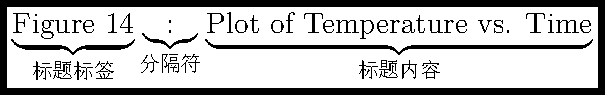
\includegraphics{captiondef}
	\caption{标题标签、分隔符和标题内容的定义}
	\label{fig:def-capcontent}
\end{fixedfigure}

\vskip2em\hrule

\paragraph{字体示例\#1}

命令
\begin{lstlisting}
\captionsetup{font={default,Large,bf}}
\caption{This is Caption Font Example \#1}
\end{lstlisting}
会将所有的标题字体重置为默认值,然后将整个标题(标签、分隔符和标题内容)设置为 \opt{Large} 字号并加粗,
而字族和字形仍然保持默认值,如图~\ref{fig:caption-font-ex1} 所示。

\begin{fixedfigure}{\linewidth}
	\centering
	\usebox{\boxgraphictwo}
	\captionsetup{font={default,Large,bf}}
	\caption{This is Caption Font Example \#1}
	\label{fig:caption-font-ex1}
\end{fixedfigure}

注意,以上的例子中的代码会同时影响图形和表格的标题。
如果 \cmd{captionsetup} 添加了 \opt{[figure]} 选项
\begin{lstlisting}
\captionsetup[figure]{font={default,Large,bf}}
\end{lstlisting}
就会只修改图形标题的字体。

\vskip2em\hrule


\paragraph{字体示例\#2}

命令
\begin{lstlisting}
\captionsetup{font=default, textfont={scriptsize,sf}}
\caption{This is Caption Font Example \#2}
\end{lstlisting}
会将所有的标题字体重置为默认值,
然后将标题内容设置为 \opt{scriptsize} 字号和无衬线字族,
如图~\ref{fig:caption-font-ex2} 所示。

\begin{fixedfigure}{\linewidth}
	\centering
	\usebox{\boxgraphictwo}
	\captionsetup{font=default, textfont={scriptsize,sf}}
	\caption{This is Caption Font Example \#2}
	\label{fig:caption-font-ex2}
\end{fixedfigure}

\vskip2em\hrule

\paragraph{字体示例\#3}

命令
\begin{lstlisting}
\captionsetup{font={default,Large}, labelfont=bf, textfont=sl}
\caption{This is Caption Font Example \#3}
\end{lstlisting}
会将所有的标题字体重置为默认值,
然后将整个标题(标题标签、分隔符和标题内容)设置为 \opt{Large} 字号,
然后将标题标签和分隔符加粗、将标题内容设置为斜体,
如图~\ref{fig:caption-font-ex3} 所示。

\begin{fixedfigure}{\linewidth}
	\centering
	\usebox{\boxgraphictwo}
	\captionsetup{font={default,Large}, labelfont=bf, textfont=sl}
	\caption{This is Caption Font Example \#3}
	\label{fig:caption-font-ex3}
\end{fixedfigure}

\vskip2em\hrule

\subsubsection{Caption垂直间距选项}\label{sssec:caption-spaceopt}

顾名思义,标题上方的间距由 \opt{aboveskip} 选项控制,
标题下方的间距由 \opt{belowskip} 选项控制。
不过,仅当使用 \opt{position=bottom} 选项时才成立。
当使用 \opt{position=top} 选项时,\opt{aboveskip} 和 \opt{belowskip} 选项的意义是相反的。
\footnote{
	注意,\opt{position=top} 只说明标题的上下间距按浮动体顶部的标题来处理,
	并不意味着标题真的位于图形或表格的上方。
	标题的实际位置取决于声明 \cmd{caption} 的位置。——译注}
遵循如下的原则可以避免发生混淆:
\begin{enumerate}
	\item 使用 \opt{skip=} 选项指定标题和浮动体内容的间距。
	\item 使用 \opt{belowskip=} 选项指定标题和周围正文的间距。
	\item 默认的选项 \opt{position=auto} 会自动判断标题的位置。
	在极少数情况下自动判断失效时,使用 \opt{position=bottom} 或 \opt{position=top} 指定标题位于浮动体底部或顶部。
\end{enumerate}

\paragraph{垂直间距示例\#1}

使用 \opt{skip=} 选项修改标题和浮动体内容的间距(默认为 $10\pt$)。
如下命令
\begin{lstlisting}
\captionsetup{skip=1cm}
\caption{Vertical Spacing Example \#1}
\end{lstlisting}
在标题和浮动体内容之间留出1厘米间距,如图~\ref{fig:caption-skip-ex1}

\begin{fixedfigure}{\linewidth}
	\centering
	\usebox{\boxgraphictwo}
	\captionsetup{skip=1cm}
	\caption{Vertical Spacing Example \#1}
	\label{fig:caption-skip-ex1}
\end{fixedfigure}

\vskip2em\hrule

\paragraph{垂直间距示例\#2}

以下例子表明 \opt{position=top} 会反转 \opt{aboveskip} 和 \opt{belowskip} 的意义。
\begin{lstlisting}
\captionsetup{aboveskip=1cm,position=top}
\caption{Vertical Spacing Example \#2}
\end{lstlisting}
如表~\ref{tab:caption-skip-ex2} 所示,标题下方的间距为1厘米\footnote{
	实际上该设置等价于 \cmdM{captionsetup}{skip=1cm}。
	这是因为当在 \env{tabular} 表格环境或者 \cmd{includegraphics} 插入命令之前使用 \cmd{caption} 时,
	默认选项 \opt{position=auto} 会自动判断为 \opt{top}。}。

\begin{fixedtable}{\linewidth}
	\centering
	\captionsetup{aboveskip=1cm,position=top}
	\caption{Vertical Spacing Example \#2}\label{tab:caption-skip-ex2}
	\begin{tabular}{|c|c|}
		\hline
		a & b \\ \hline
		c & d \\ \hline
	\end{tabular}
\end{fixedtable}

\vskip2em\hrule

\paragraph{垂直间距示例\#3}

一般而言,表格标题位于表格上方,而图形标题位于图形的下方。
因此,为方便起见可以分别为表格和图形设置标题位置。
\begin{lstlisting}
\captionsetup{skip=1cm,belowskip=0pt}
\captionsetup[figure]{position=bottom}
\captionsetup[table]{position=top}
...
\caption{Table for Vertical Spacing Example \#3}
\caption{Figure for Vertical Spacing Example \#3}
\end{lstlisting}
\pkg{caption} 宏包还专门提供了宏包选项 \opt{figureposition} 和 \opt{tableposition} 作为以上命令的缩写。上述命令等价于
\begin{lstlisting}
\usepackage[...,figureposition=bottom,tableposition=top]{caption}
\captionsetup{skip=1cm,belowskip=0pt}
...
\caption{Table for Vertical Spacing Example \#3}
\caption{Figure for Vertical Spacing Example \#3}
\end{lstlisting}
这样表格的标题下方有1厘米间距(表~\ref{tab:caption-skip-ex3}),
而图形的标题上方有1厘米间距(图~\ref{fig:caption-skip-ex3})。

\begin{fixedfigure}{\linewidth}
	\centering
	\captionsetup{type=table}
	\captionsetup{skip=1cm,belowskip=0pt}
%	\captionsetup[table]{position=top}
	\caption{Table for Vertical Spacing Example \#3}
	\label{tab:caption-skip-ex3}
	\begin{tabular}{|c|c|}
		\hline
		a & b \\ \hline
		c & d \\ \hline
	\end{tabular}\\
	\usebox{\boxgraphictwo}
	\captionsetup{type=figure}
%	\captionsetup[figure]{position=bottom}
	\caption{Figure for Vertical Spacing Example \#3}
	\label{fig:caption-skip-ex3}
\end{fixedfigure}

\vskip2em\hrule

\subsubsection{Caption 宏包标签选项}\label{sssec:caption-labelopt}

\paragraph{标签选项示例\#1}

\begin{lstlisting}
\captionsetup{labelformat=simple}
\caption{This is Caption Label Example \#1}
\end{lstlisting}
如图~\ref{fig:caption-label-ex1} 所示,标签格式设置为 \opt{simple}。
一般情况下 \opt{simple} 格式等同于 \opt{default} 格式,
除非文档类重新定义了 \opt{default} 为不同样式。

\begin{fixedfigure}{\linewidth}
	\centering
	\usebox{\boxgraphictwo}
	\captionsetup{labelformat=simple}
	\caption{This is Caption Label Example \#1}
	\label{fig:caption-label-ex1}
\end{fixedfigure}

\vskip2em\hrule

\paragraph{标签选项示例\#2}

\begin{lstlisting}
\captionsetup{labelformat=parens}
\caption{This is Caption Label Example \#2}
\end{lstlisting}
如图~\ref{fig:caption-label-ex2} 所示,标签格式为 \opt{parens}。
数字编号位于一对圆括号内。

\begin{fixedfigure}{\linewidth}
	\centering
	\usebox{\boxgraphictwo}
	\captionsetup{labelformat=parens}
	\caption{This is Caption Label Example \#2}
	\label{fig:caption-label-ex2}
\end{fixedfigure}

\vskip2em\hrule

\paragraph{标签选项示例\#3}

\begin{lstlisting}
\captionsetup{labelformat=empty, labelsep=none}
\caption{This is Caption Label Example \#3}
\end{lstlisting}
如图~\ref{fig:caption-label-ex3} 所示,标签格式为 \opt{empty}。
不过由于没有编号,很难说这是图~\ref{fig:caption-label-ex3}。

\begin{fixedfigure}{\linewidth}
	\centering
	\usebox{\boxgraphictwo}
	\captionsetup{labelformat=empty, labelsep=none}
	\caption{This is Caption Label Example \#3}
	\label{fig:caption-label-ex3}
\end{fixedfigure}

\vskip2em\hrule

\paragraph{标签选项示例\#4}

\begin{lstlisting}
\captionsetup{labelformat=default, labelsep=period}
\caption{This is Caption Label Example \#4}
\end{lstlisting}
如图~\ref{fig:caption-label-ex4} 所示,标题分隔符由默认的冒号改为句点。

\begin{fixedfigure}{\linewidth}
	\centering
	\usebox{\boxgraphictwo}
	\captionsetup{labelformat=default, labelsep=period}
	\caption{This is Caption Label Example \#4}
	\label{fig:caption-label-ex4}
\end{fixedfigure}

\vskip2em\hrule

\paragraph{标签选项示例\#5}

\begin{lstlisting}
\captionsetup{labelformat=default, labelsep=newline}
\caption{This is Caption Label Example \#5}
\end{lstlisting}
如图~\ref{fig:caption-label-ex5} 所示,标题分隔符改成另起一行。

\begin{fixedfigure}{\linewidth}
	\centering
	\usebox{\boxgraphictwo}
	\captionsetup{labelformat=default, labelsep=newline}
	\caption{This is Caption Label Example \#5}
	\label{fig:caption-label-ex5}
\end{fixedfigure}

\vskip2em\hrule

\subsubsection{Caption 宏包格式选项}\label{sssec:caption-formatopt}

\paragraph{格式选项示例\#1:标题宽度}

\begin{lstlisting}
\captionsetup{width=3in}
\caption{This is an example of customizing the caption width}
\end{lstlisting}
如图~\ref{fig:caption-format-ex1} 所示,标题宽度设置为 3英寸。

\begin{fixedfigure}{\linewidth}
	\centering
	\usebox{\boxgraphictwo}
	\captionsetup{width=3in}
	\caption{This is an example of customizing the caption width}
	\label{fig:caption-format-ex1}
\end{fixedfigure}

\vskip2em\hrule

\paragraph{格式选项示例\#2:默认格式}

图~\ref{fig:caption-format-ex2-justified}--\ref{fig:caption-format-ex2-raggedleft} 展示了在 \opt{format=default} 格式下,七种不同的 \opt{justification=} 的效果。
这些图由如下代码生成:
\begin{lstlisting}
\captionsetup{format=default,justification=justified}
\caption{Caption with default format and justified justification.
Caption with default format and justified justification.
Caption with default format and justified justification.}
...
\captionsetup{format=default,justification=centering}
\caption{Caption with default format and centering justification.
Caption with default format and centering justification.
Caption with default format and centering justification.}
...
\captionsetup{format=default,justification=centerlast}
\caption{Caption with default format and centerlast justification.
Caption with default format and centerlast justification.
Caption with default format and centerlast justification.}
...
\captionsetup{format=default,justification=centerfirst}
\caption{Caption with default format and centerfirst justification.
Caption with default format and centerfirst justification.
Caption with default format and centerfirst justification.}
...
\captionsetup{format=default,justification=raggedright}
\caption{Caption with default format and raggedright justification.
Caption with default format and raggedright justification.
Caption with default format and raggedright justification.}
...
\captionsetup{format=default,justification=RaggedRight}
\caption{Caption with default format and RaggedRight justification.
Caption with default format and RaggedRight justification.
Caption with default format and RaggedRight justification.}
...
\captionsetup{format=default,justification=raggedleft}
\caption{Caption with default format and raggedleft justification.
Caption with default format and raggedleft justification.
Caption with default format and raggedleft justification.}
\end{lstlisting}
从图~\ref{fig:caption-format-ex2-justified}--\ref{fig:caption-format-ex2-raggedleft} 中可以看出,
标题的第一行与其它行的格式是一样的。

\begin{figure}[tp]
	\centering
	\begin{minipage}{0.45\linewidth}
		\usebox{\boxgraphictwo}
		\captionsetup{format=default,justification=justified}
		\caption{Caption with default format and justified justification.
			Caption with default format and justified justification.
			Caption with default format and justified justification.}
		\label{fig:caption-format-ex2-justified}
	\end{minipage}\\[1em]
	\begin{minipage}{0.45\linewidth}
		\usebox{\boxgraphictwo}
		\captionsetup{format=default,justification=centering}
		\caption{Caption with default format and centering justification.
			Caption with default format and centering justification.
			Caption with default format and centering justification.}
		\label{fig:caption-format-ex2-centering}
	\end{minipage}\hfill
	\begin{minipage}{0.45\linewidth}
		\usebox{\boxgraphictwo}
		\captionsetup{format=default,justification=centerlast}
		\caption{Caption with default format and centerlast justification.
			Caption with default format and centerlast justification.
			Caption with default format and centerlast justification.}
		\label{fig:caption-format-ex2-centerlast}
	\end{minipage}\\[1em]
	\begin{minipage}{0.45\linewidth}
		\usebox{\boxgraphictwo}
		\captionsetup{format=default,justification=centerfirst}
		\caption{Caption with default format and centerfirst justification.
			Caption with default format and centerfirst justification.
			Caption with default format and centerfirst justification.}
		\label{fig:caption-format-ex2-centerfirst}
	\end{minipage}\hfill
	\begin{minipage}{0.45\linewidth}
		\usebox{\boxgraphictwo}
		\captionsetup{format=default,justification=raggedright}
		\caption{Caption with default format and raggedright justification.
			Caption with default format and raggedright justification.
			Caption with default format and raggedright justification.}
		\label{fig:caption-format-ex2-raggedright}
	\end{minipage}\\[1em]
	\begin{minipage}{0.45\linewidth}
		\usebox{\boxgraphictwo}
		\captionsetup{format=default,justification=RaggedRight}
		\caption{Caption with default format and RaggedRight justification.
			Caption with default format and RaggedRight justification.
			Caption with default format and RaggedRight justification.}
		\label{fig:caption-format-ex2-RaggedRight}
	\end{minipage}\hfill
	\begin{minipage}{0.45\linewidth}
		\usebox{\boxgraphictwo}
		\captionsetup{format=default,justification=raggedleft}
		\caption{Caption with default format and raggedleft justification.
			Caption with default format and raggedleft justification.
			Caption with default format and raggedleft justification.}
		\label{fig:caption-format-ex2-raggedleft}
	\end{minipage}
\end{figure}

\vskip2em\hrule

\paragraph{格式选项示例\#3:悬挂模式}

图~\ref{fig:caption-format-ex3-justified}--\ref{fig:caption-format-ex3-raggedleft} 展示了在 \opt{format=hang} 格式下,七种不同的 \opt{justification=} 的效果。
这些图由如下代码生成:
\begin{lstlisting}
\captionsetup{format=hang,indention=0pt,justification=justified}
\caption{Caption with hang format and justified justification.
Caption with hang format and justified justification.
Caption with hang format and justified justification.}
...
\captionsetup{format=hang,indention=0pt,justification=centering}
\caption{Caption with hang format and centering justification.
Caption with hang format and centering justification.
Caption with hang format and centering justification.}
...
\captionsetup{format=hang,indention=0pt,justification=centerlast}
\caption{Caption with hang format and centerlast justification.
Caption with hang format and centerlast justification.
Caption with hang format and centerlast justification.}
...
\captionsetup{format=hang,indention=0pt,justification=centerfirst}
\caption{Caption with hang format and centerfirst justification.
Caption with hang format and centerfirst justification.
Caption with hang format and centerfirst justification.}
...
\captionsetup{format=hang,indention=0pt,justification=raggedright}
\caption{Caption with hang format and raggedright justification.
Caption with hang format and raggedright justification.
Caption with hang format and raggedright justification.}
...
\captionsetup{format=hang,indention=0pt,justification=RaggedRight}
\caption{Caption with hang format and RaggedRight justification.
Caption with hang format and RaggedRight justification.
Caption with hang format and RaggedRight justification.}
...
\captionsetup{format=hang,indention=0pt,justification=raggedleft}
\caption{Caption with hang format and raggedleft justification.
Caption with hang format and raggedleft justification.
Caption with hang format and raggedleft justification.}
\end{lstlisting}
从图~\ref{fig:caption-format-ex3-justified}--\ref{fig:caption-format-ex3-raggedleft} 中可以看出,
\opt{format=hang} 效果是:标题从第二行有额外的缩进。
标题的第一行与其它行的格式是一样的。

\begin{figure}[tp]
	\centering
	\begin{minipage}{0.45\linewidth}
		\usebox{\boxgraphictwo}
		\captionsetup{format=hang,indention=0pt,justification=justified}
		\caption{Caption with hang format and justified justification.
			Caption with hang format and justified justification.
			Caption with hang format and justified justification.}
		\label{fig:caption-format-ex3-justified}
	\end{minipage}\\[1em]
	\begin{minipage}{0.45\linewidth}
		\usebox{\boxgraphictwo}
		\captionsetup{format=hang,indention=0pt,justification=justified}
		\caption{Caption with hang format and justified justification.
			Caption with hang format and justified justification.
			Caption with hang format and justified justification.}
		\label{fig:caption-format-ex3-centering}
	\end{minipage}\hfill
	\begin{minipage}{0.45\linewidth}
		\usebox{\boxgraphictwo}
		\captionsetup{format=hang,indention=0pt,justification=centerlast}
		\caption{Caption with hang format and centerlast justification.
			Caption with hang format and centerlast justification.
			Caption with hang format and centerlast justification.}
		\label{fig:caption-format-ex3-centerlast}
	\end{minipage}\\[1em]
	\begin{minipage}{0.45\linewidth}
		\usebox{\boxgraphictwo}
		\captionsetup{format=hang,indention=0pt,justification=centerfirst}
		\caption{Caption with hang format and centerfirst justification.
			Caption with hang format and centerfirst justification.
			Caption with hang format and centerfirst justification.}
		\label{fig:caption-format-ex3-centerfirst}
	\end{minipage}\hfill
	\begin{minipage}{0.45\linewidth}
		\usebox{\boxgraphictwo}
		\captionsetup{format=hang,indention=0pt,justification=raggedright}
		\caption{Caption with hang format and raggedright justification.
			Caption with hang format and raggedright justification.
			Caption with hang format and raggedright justification.}
		\label{fig:caption-format-ex3-raggedright}
	\end{minipage}\\[1em]
	\begin{minipage}{0.45\linewidth}
		\usebox{\boxgraphictwo}
		\captionsetup{format=hang,indention=0pt,justification=RaggedRight}
		\caption{Caption with hang format and RaggedRight justification.
			Caption with hang format and RaggedRight justification.
			Caption with hang format and RaggedRight justification.}
		\label{fig:caption-format-ex3-RaggedRight}
	\end{minipage}\hfill
	\begin{minipage}{0.45\linewidth}
		\usebox{\boxgraphictwo}
		\captionsetup{format=hang,indention=0pt,justification=raggedleft}
		\caption{Caption with hang format and raggedleft justification.
			Caption with hang format and raggedleft justification.
			Caption with hang format and raggedleft justification.}
		\label{fig:caption-format-ex3-raggedleft}
	\end{minipage}
\end{figure}


\subsection{进一步定制}\label{ssec:furthercustom}

\pkg{caption} 宏包还有一些额外的特性,可以允许用户进行进一步的定制。
本节对此进行了简要介绍,详细的指南请参考 \cite{caption-doc}。

\subsubsection{标题样式}\label{sssec:caption-style}

用户可以定义一组标题选项,称之为\emph{标题样式}。
这样通过一个样式选项就可以指定一组选项值。
例如,\opt{caption} 宏包已经定义了名为 \opt{default} 的选项:
\begin{lstlisting}
\captionsetup{style=default}
\end{lstlisting}
就等价于
\begin{lstlisting}
\captionsetup{font=default, labelfont=default,
textfont=default, parskip=0pt,
labelformat=simple, labelsep=colon,
format=default, indentation=0pt,
hangindent=0pt, margin=0pt,
parinident=0pt, justification=justified,
singlelinecheck=true}
\end{lstlisting}
可以在导言区使用 \cmdi{DeclareCaptionStyle} 命令来定义其它标题样式。
这些样式既可以是显式地定义所有的参数值,
也可以从默认样式出发只修改个别的选项值。
例如,在导言区中使用如下 \cmd{DeclareCaptionStyle} 命令
\begin{lstlisting}
\DeclareCaptionStyle{BigLeft}{style=default, labelsep=period,
font=Large, labelfont=bf,
justification=RaggedRight,
singlelinecheck=false}
\end{lstlisting}
就可以通过如下命令使用 \opt{BigLeft} 样式
\begin{lstlisting}
\captionsetup{style=BigLeft}
\caption{This Caption uses BigLeft Style}
\end{lstlisting}
效果如图~\ref{fig:caption-style-BigLeft}

\begin{fixedfigure}{\linewidth}
	\centering
	\usebox{\boxgraphictwo}
	\captionsetup{style=BigLeft}
	\caption{This Caption uses BigLeft Style}
	\label{fig:caption-style-BigLeft}
\end{fixedfigure}

\vskip2em\hrule

\subsubsection{其它选项值}\label{sssec:caption-addoptval}

\pkg{caption} 宏包提供了一组命令用于其它的选项值,这些命令只能用于导言区中。
\begin{lstlisting}
\DeclareCaptionFont
\DeclareCaptionLabelSeparator
\DeclareCaptionLabelFormat
\DeclareCaptionFormat
\DeclareCaptionJustification
\DeclareCaptionTextFormat
\end{lstlisting}

\paragraph{选项定义示例\#1}

表~\ref{tab:caption-fontval} 定义了可以用于 \opt{font=}、\opt{labelfont=}和 \opt{textfont=} 选项的字体选项值。
\cmdi{DeclareCaptionFont} 命令允许用户定义额外的字体选项值。
例如,在导言区使用如下命令会定义一个 \opt{BigAndBold} 选项值
\begin{lstlisting}
\DeclareCaptionFont{BigAndBold}{\Large\bfseries}
\end{lstlisting}
然后可以使用如下代码
\begin{lstlisting}
\captionsetup{font=BigAndBold}
\caption{This Caption uses a Custom Font}
\end{lstlisting}
效果如图~\ref{fig:caption-font-BigAndBold} 所示。

\begin{fixedfigure}{\linewidth}
	\centering
	\usebox{\boxgraphictwo}
	\captionsetup{font=BigAndBold}
	\caption{This Caption uses a Custom Font}
	\label{fig:caption-font-BigAndBold}
\end{fixedfigure}

\vskip2em\hrule

\paragraph{选项定义示例\#2}

表~\ref{tab:caption-labelopt} 描述了如何用 \opt{labelformat=} 选项控制标题的表头(例如“Figure 33”)部分的格式。
\cmdi{DeclareCaptionLabelFormat} 命令允许用户自定义额外的 \opt{labelformat=} 选项。
在自定义中,使用符号 \opt{\#1} 和 \opt{\#2} 指定表头(例如“Figure”)和数字编号的插入地点。
例如,在导言区使用如下命令会定义一个 \opt{hash} 选项值
\begin{lstlisting}
\DeclareCaptionLabelFormat{hash}{#1 {\#}#2}
\end{lstlisting}
效果是在数字编号之前使用符号 \# 。
不过,该定义有一个小瑕疵,如果 \opt{\#1} 为空的话,在\opt{\#1} 后面的空格是不必要的。
因此,\pkg{caption} 宏包提供了两个辅助命令。
\cmdi{bothIfFirst} 命令有两个变量,只有当第一个变量不为空时才输出这两个变量,
否则都不会输出。
类似地,\cmdi{bothIfSecond} 仅当第二个变量不为空时才输出这两个变量,否则都不会输出。
使用 \cmd{bothIfFirst} 命令后的定义是
\begin{lstlisting}
\DeclareCaptionLabelFormat{hash}{\bothIfFirst{#1}{ }{\#}#2}
\end{lstlisting}
该定义要放在导言区,之后可以设置标题格式
\begin{lstlisting}
\captionsetup{labelformat=hash}
\caption{This Caption has a Custom Label Format}
\end{lstlisting}
效果如图~\ref{fig:caption-labelformat-hash}。

\begin{fixedfigure}{\linewidth}
	\centering
	\usebox{\boxgraphictwo}
	\captionsetup{labelformat=hash}
	\caption{This Caption has a Custom Label Format}
	\label{fig:caption-labelformat-hash}
\end{fixedfigure}

\vskip2em\hrule

\paragraph{选项定义示例\#3}

表~\ref{tab:caption-labelopt} 定义了 \opt{labelsep=} 接受的选项值。
此外,用户还可以使用 \cmdi{DeclareCaptionLabelSeparator} 命令为 \opt{labelsep=} 选项自定义额外的选项值。
例如,在导言区使用如下命令会将标签分隔符定义为箭头
\begin{lstlisting}
\DeclareCaptionLabelSeparator{arrow}{\quad\ensuremath{\Rightarrow}\quad}
\end{lstlisting}
之后如下代码
\begin{lstlisting}
\captionsetup{labelsep=arrow}
\caption{This Caption has a Custom Label Separator}
\end{lstlisting}
的效果见图~\ref{fig:caption-labelformat-arrow}。

\begin{fixedfigure}{\linewidth}
	\centering
	\usebox{\boxgraphictwo}
	\captionsetup{labelsep=arrow}
	\caption{This Caption has a Custom Label Separator}
	\label{fig:caption-labelformat-arrow}
\end{fixedfigure}

\vskip2em\hrule

\paragraph{选项定义示例\#4}

表~\ref{tab:caption-formatopt} 介绍了 \opt{format=} 选项值。
\cmdi{DeclareCaptionFormat} 命令允许用户为 \opt{format=} 选项自定义额外的选项值。
在自定义中,使用符号 \opt{\#1}、\opt{\#2} 和 \opt{\#3} 指代标题的各部分。
其中 \opt{\#1} 代表标题标签,\opt{\#2} 代表标题分隔符,\opt{\#3} 代表标题文本(其定义可参见图~\ref{fig:def-capcontent})。
例如,在导言区使用如下命令定义了 \opt{reverse} 格式,
使得先出现标题内容,然后是标题分隔符,最后是放在双尖括号 \cmd{ll} 和 \cmd{gg} 内的标题标签。
\begin{lstlisting}
\DeclareCaptionFormat{reverse}{#3#2\ensuremath{\ll}#1\ensuremath{\gg}}
\end{lstlisting}
之后如下代码
\begin{lstlisting}
\captionsetup{format=reverse,labelsep=empty}
\caption{This Caption has a Custom Format}
\end{lstlisting}
的效果见图~\ref{fig:caption-format-reverse}。

\begin{fixedfigure}{\linewidth}
	\centering
	\usebox{\boxgraphictwo}
	\captionsetup{format=reverse,labelsep=none}
	\caption{This Caption has a Custom Format}
	\label{fig:caption-format-reverse}
\end{fixedfigure}


\section{不浮动的图形}\label{sec:nonfloat}

\emph{由于不浮动的图形会生成大段的垂直空白,因此一般认为是比较糟糕的排版风格。
	此时强烈建议用户使用 \env{figure} 环境的 \opt{[!ht]} 选项,
	这样只有当当前页面排不下时才会移动图形。}

如同第~\ref{sec:floatfigure}~节所介绍的那样,
\LaTeX{} 允许“浮动”的图形和表格以增强排版效果。
不过,偶尔也会希望一幅图形不要浮动,就放置在与它在 \LaTeX{} 源文件中相同的位置。
虽然 \cmd{caption} 命令只能在 \env{figure} 和 \env{table} 环境中使用,
但是 \pkg{caption} 宏包定义了 \cmd{captionof} 命令,
该命令有两个选项:标题的类型(表格、图形等)以及标题的内容,
这样就可以在 \env{figure} 和 \env{table} 环境之外使用了。
使用命令
\begin{lstlisting}
\captionof{figure}{caption text}
\end{lstlisting}
就可以创建一个图形标题,而不用关心是否真的出现在 \env{figure} 环境中。
类似地,使用命令
\begin{lstlisting}
\captionof{table}{caption text}
\end{lstlisting}
会创建一个表格标题。
而如下的命令
\begin{lstlisting}
This is the text before the figure.
\\[\intextsep]
\begin{minipage}{\linewidth}
	\centering
	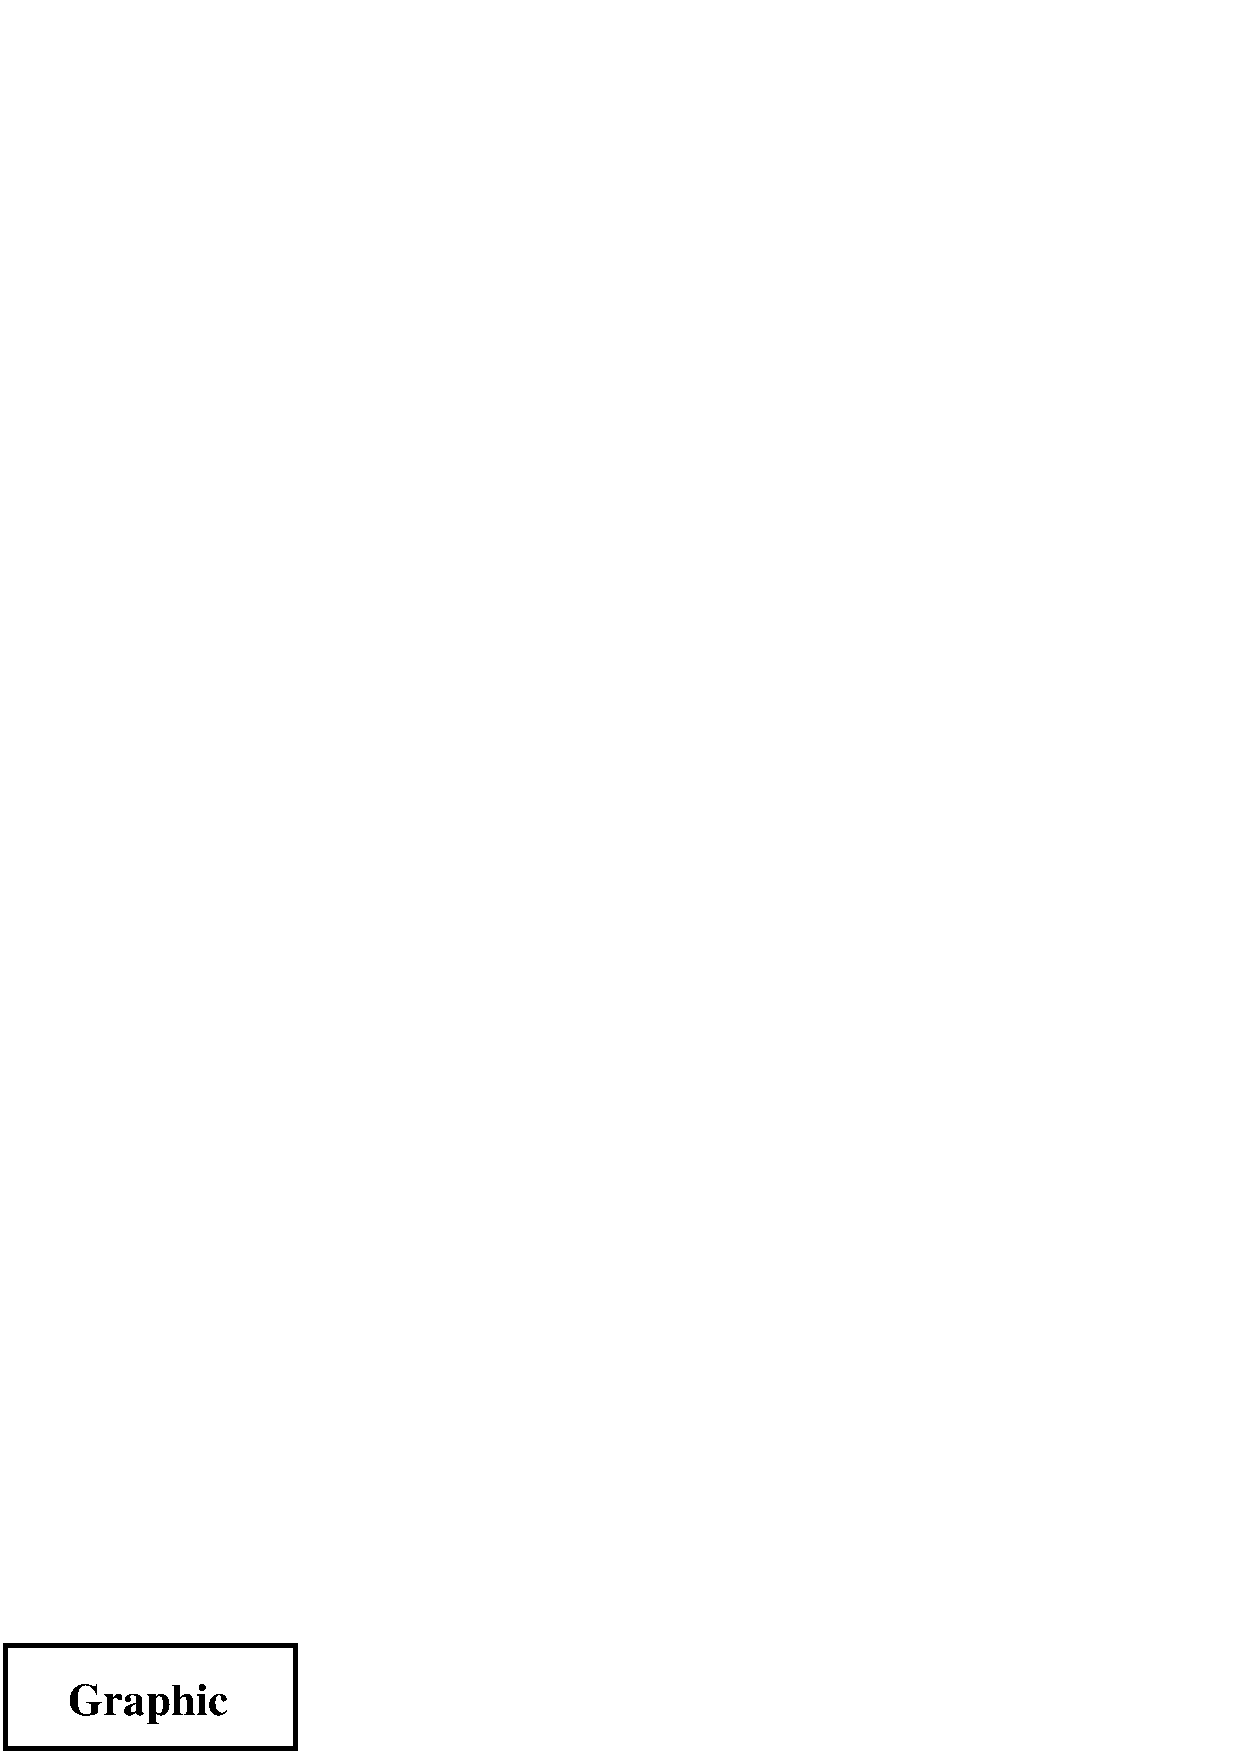
\includegraphics[width=2in]{graphic}%
	\captionof{figure}{This is a non-floating figure}
	\label{fig:non:float}
\end{minipage}
\\[\intextsep]
This is the text after the figure.
\end{lstlisting}
可得到一幅不浮动的图形。对于不浮动的图形,需要注意下面几点:
\begin{itemize}
	\item 需要使用 \env{minipage} 小页环境来防止在图形中出现分页的情况。
	\item 图形前后的命令 \cmdO{\cmd{}}{\cmd{intextsep}} 作用是进行换行并加上垂直的间距。
	\cmd{intextsep} 命令~(见第~\ref{ssec:vspace}~节)可以使用任意大小的空白,
	目的是使不浮动的图形具有与浮动图形相同的上下间距。
	\item 正常情况下,浮动图形是按照它们在 \LaTeX{} 源文件中的顺序一一被放置的。
	而不浮动的图形是被立即放置到页面上,
	所以可以跳过浮动图形队列中的未处理图形。
	如果出现这样情况,那么图形不会按照数字顺序编号\footnote{
		在这种情况下,图形目录中图形的顺序是按照图形出现的顺序,而不是图形编号的顺序。}。
	要避免这种顺序错乱,可在不浮动的图形前用 \cmd{clearpage} 或 \cmd{FloatBarrier} 命令
	清除未处理的浮动图形(见第~\ref{ssec:unprocessfig}~节)。
	\item \cmd{captionof} 命令也可以用于生成边注图形
	(见第~\ref{sec:marginfigure}~节)以及与图形并列的表格
	(见第~\ref{sec:figuretable} 节)。
\end{itemize}

\subsection{不使用 caption 宏包的非浮动图形}\label{ssec:nonfloat-nocaption}

以上篇幅介绍了如何使用 \pkg{caption} 宏包的 \cmd{captionof} 命令来创建 \env{figure}/\env{table} 环境之外的标题。
本节介绍如何不使用 \pkg{caption} 宏包做到这一点。

\cmd{caption} 命令之所以可以在 \env{figure} 和 \env{table} 环境中使用,
是因为这两个环境分别为图形和表格定义了内部命令 \cmdi{@captype}。
这样,通过定义 \cmd{@captype} 就可以在 \env{figure} 和 \env{table} 环境外使用 \cmd{caption} 命令。
当然这时 \cmd{@captype} 必须用 \cmd{makeatletter}-\cmd{makeatother} 命令对包围起来,
使得可以在命令名中使用 \texttt{@}。
当然,可以每次都使用如下的命令:
\begin{lstlisting}
\includegraphics{file} 
\makeatletter\def\@captype{figure}\makeatother 
\caption{This is the caption}
\end{lstlisting}
不过,更方便的做法是在导言区中定义下面的命令:
\begin{lstlisting}
\makeatletter 
\newcommand\figcaption{\def\@captype{figure}\caption} 
\newcommand\tabcaption{\def\@captype{table}\caption} 
\makeatother
\end{lstlisting}
这样定义了两个命令 \cmd{figcaption} 和 \cmd{tabcaption}。
在正文中无论是否在图形环境中,都可用 \cmd{figcaption} 得到图形标题。
同样地,无论是否在表格环境中,都可用 \cmd{tabcaption} 得到表格标题。

\subsection{float 宏包中的 [H] 位置选项}

\pkgi{float} 宏包\footnote{
	\pkg{float} 宏包允许用户新的浮动体,如 \env{Program}、\env{Algorithm} 等。
	也可以定制加框的和加线条的浮动式样。
	这些可选的浮动式样重定义了 \cmd{caption} 命令,
	使得无论将 \cmd{caption} 命令放在何处,
	总会在特定的地方排版标题,因此不可以创建并列图形以及其它的复杂图形。}
为 \env{figure} 环境加上了一个 \opt{[H]} 位置选项,
从而使得用 \env{figure} 环境可以生成不浮动的图形。
如下代码
\begin{lstlisting}
\usepackage{float}
...
\begin{figure}[H]
	.....
\end{figure}
\end{lstlisting}
可以生成不浮动的图形。

如果当前页没有足够的空间放置一幅使用了 \opt{[H]} 位置选项的图形,
该图形会被置于下一页的顶部。
如果当前页中有脚注的话,它将会紧接在文本后排出,而不是像通常那样置于页面的底部。
如果不想要这种效果,可以使用第~\ref{sec:nonfloat} 节介绍的 \cmd{captionof} 命令来代替 \pkg{float} 宏包的 \opt{[H]} 位置选项。


\section{边注图形}\label{sec:marginfigure}

\cmdi{marginpar} 命令可以用来生成边注。
除非使用了 \cmdi{reversemarginpar} 命令(本文档就用了该命令),
边注一般放在页面的右边(在 \opt{twoside} 格式的文档中放在页面的外侧)。
边注的宽度由长度 \cmdi{marginparwidth} 控制,
而与正文之间的水平距离由 \cmdi{marginparsep} 决定。

边注的第一行与包含 \cmd{marginpar} 命令的正文文本的那一行对齐
(边注的第一行的参考点与当前基线对齐)。

边注不能分页,如果一个边注靠近页面的底部而无法正常排下时,
它会伸入页面的底边空白继续排出。
如果前面一个边注干扰了后面的边注,
那么 \LaTeX{} 会把后面的边注向下移动,但不会移到下一页。
所以在最后完成排版前可能要调整一下边注的位置以防它离分页的地方太近。

由于 \env{figure}~环境不能在边注中使用,
所以无法直接得到浮动的边注图形。
这时,可以用第~\ref{sec:nonfloat}~节定义的 \cmd{captionof} 命令来构造非浮动的边注图形。
\marginpar{\centering
	\resizebox{\marginparwidth}{!}{\usebox{\boxgraphic}}%
	\captionsetup{type=figure}
	\caption{这是边注图形}
	\label{fig:marginal:fig} }
例如,图~\ref{fig:marginal:fig} 就由下面的命令来得到:
\begin{lstlisting}
... 构造非浮动的边注图形。
\marginpar{\centering 
	\includegraphics[width=\marginparwidth]{graphic.eps}% 
	\captionsetup{type=figure}
	\caption{This is a Marginal Figure} 
	\label{fig:marginal:fig} }
例如,图~\ref{fig:marginal:fig} 就由下面的命令来得到:
\end{lstlisting}

图~\ref{fig:marginal:fig} 中图像底部与 \cmd{marginpar} 命令所在文本的基线是对齐的。
对于使用边注图形,需要注意的是:
\begin{itemize}	
	\item 由于边注图形都比较窄小,所以在 \cmd{caption} 命令之前使用 \pkg{caption} 宏包命令
\begin{lstlisting}
\captionstyle{justification=raggedright}
\captionstyle{justification=raggedleft}
\end{lstlisting}
	可能会得到更好的标题格式效果。
	此外,\pkg{caption} 宏包命令
\begin{lstlisting}
\captionsetup{font=small}
\end{lstlisting}
	可以减小标题的字体。
	关于 \pkg{caption} 的信息详见第~\ref{sec:caption-pkg} 节。
	
	\item 如同第~\ref{sec:nonfloat}~节所介绍的非浮动图形,
	边注图形会在未处理的浮动图形前排出。
	因此,如果希望图形按顺序出现的话,
	必须在边注之前使用 \cmd{clearpage} 或 \cmd{FloatBarrier} 命令。
	
	\item 边注的处理机制和浮动图表的处理机制是一样的,
	所以如果使用了太多的浮动图表和边注,
	就可能超出 \LaTeX{} 所允许的未处理的浮动体的数目。
	这时使用 \pkg{morefloat}~宏包是一种解决办法。
	具体见第~\ref{ssec:toomanyfig} 节。
\end{itemize}      

\section{宽图形的处理} \label{sec:widefig}

排版的易读性原则限制了一行文本中的字符个数。
如果不是使用大字体或双列版式,这样的易读性原则就会使得页面的页边距很大,
特别当使用 $8.5\times 11 $ 英寸的 letter 页面时更是如此。
在第~\ref{sec:marginfigure}~节中展示了边空可以用来放置边注图形。
另外一种方法则是创建一个常规的浮动图形,并且伸到一边或者两边的边空中。
这可通过在浮动图形环境中嵌套一个很宽的列表环境来实现。
例如,可以在导言区加入下列代码来定义一个 \env{narrow} 环境:
\begin{lstlisting}
\newenvironment{narrow}[2]{%
	\begin{list}{}{%
		\setlength{\topsep}{0pt}%
		\setlength{\leftmargin}{#1}%
		\setlength{\rightmargin}{#2}%
		\setlength{\listparindent}{\parindent}%
		\setlength{\itemindent}{\parindent}%
		\setlength{\parsep}{\parskip}}%
	\item[]}{\end{list}}
\end{lstlisting}

那么,所有位于 \cmdOOM{begin}{narrow}{1in}{2in} 和 \cmdM{end}{narrow} 之间的文本都被向左缩进1英寸,向右缩进2英寸。
当使用负长度时,文本就会延伸到边空上去。

\subsection{单面版式中的宽图形}\label{ssec:widefig-oneside}

在使用单面版式排版时,页面左右的边空不会因奇偶页而取不同的值,
故可以不用考虑图形浮动到奇数页或偶数页的问题。
下面的命令利用前面定义的 \env{narrow} 环境使得图形左边延伸到左边空中1英寸,见图~\ref{fig:widefig}。
\begin{lstlisting}
\begin{figure}
	\begin{narrow}{-1in}{0in}
		
\includegraphics[width=\linewidth]{wide}
		\caption{这是宽图形}
	\end{narrow}
\end{figure}
\end{lstlisting}
这里给定宽度参数为 \cmd{linewidth} 使得图形的宽度和 \env{narrow} 环境的宽度相等。
若给定宽度参数为 \cmd{textwidth} 会使图形的宽度和原来的正文宽度一样。

\begin{figure}
	\begin{narrow}{-1in}{0in}
		
\includegraphics[width=\linewidth]{wide}
		\caption{这是宽图形}\label{fig:widefig}
	\end{narrow}
\end{figure}

当使用边注时,可能希望宽图形能够精确地延伸到边注的边界
(使得图形的宽度为 $\text{\cmd{linewidth}}+\text{\cmd{marginparwidth}}+\text{\cmd{marginparsep}}$)。这时可以定义新长度 \cmd{marginwidth} 并将它设为 $\text{\cmd{marginparwidth}}+\text{\cmd{marginparsep}}$。
例如:
\begin{lstlisting}
\newlength{\marginwidth} 
\setlength{\marginwidth}{\marginparwidth} 
\addtolength{\marginwidth}{\marginparsep}
\end{lstlisting}
接着在 \cmdM{begin}{narrow} 的选项中使用 \opt{-\cmd{marginwidth}} 来达到目的。

\subsection{双面版式中的宽图形}\label{widefig-twoside}

在使用双面版式排版时,页面左右的边空因奇偶页而取不同的值,
且使用宽图形时常常希望图形延伸到装订的那一边
(奇数页的左边,偶数页的右边)。
在这种情形下,需要使用 \pkg{ifthen} 宏包提供的 \cmd{ifthenelse} 命令,
进而根据图形出现在奇数页或偶数页而选取不同的命令。
例如:
\begin{lstlisting}
\usepackage{ifthen}
...
\begin{figure}
	\ifthenelse{\isodd{\pageref{fig:wide}}}%
	{% BEGIN ODD-PAGE FIGURE
		\begin{narrow}{0in}{-1in}
			\includegraphics[width=\linewidth]{file}
			\caption{Figure Caption}
			\label{fig:wide}
		\end{narrow}
	}% END ODD-PAGE FIGURE
	{% BEGIN EVEN-PAGE FIGURE
		\begin{narrow}{-1in}{0in}
			\includegraphics[width=\linewidth]{file}
			\caption{Figure Caption}
			\label{fig:wide}
		\end{narrow}
	}% END EVEN-PAGE FIGURE
\end{figure}
\end{lstlisting}
由于 \cmd{ifthenelse} 使用命令 \cmd{pageref} 作为输入,
所以需要 \LaTeX{} 运行足够的次数后才能正确地排出交叉引用。


\section{横排的图形}\label{sec:lscapefig}

在竖排版的文档中,有三种方法可以得到横排的图形。
\begin{enumerate}
	\item \pkgi{lscape} 宏包提供了一个 \envi{landscape} 环境,
	将纸张的左边界作为页面的顶部,使得在此环境中的文本,表格和图形都被横排。
	\item \pkgi{rotating} 宏包提供了一个 \envi{sidewaysfigure} 环境,
	与 \env{figure} 环境相似,只是其中的图形被横排。
	\item \pkg{rotating} 宏包提供了一个 \cmdi{rotcaption}~命令,
	与 \cmd{caption} 命令相似,只是标题被横排。
\end{enumerate}

以上三种方法的区别:
\begin{itemize}
	\item 方法1和2将横排的图形放到单独的一页上,
	而方法3则生成独立的浮动体,并不需要单独一页来放置。
	\item 方法2只是将其中的图形横排,
	而方法1中的 \env{landscape} 环境是一种通用环境,可以横排任何文本、图形和表格。
	\env{landscape} 环境还具有分页的能力,可连续生成多个横排页面\footnote
		{\env{landscape} 环境能很好地与 \pkgi{longtable} 宏包配合使用,
		从而得到连续多页横排的超长表格。}。
	\item 使用方法2得到的整页图形可以浮动以达到更好的排版效果,
	而方法1得到的图形是不能浮动的\footnote{
		在 \env{landscape}环境中声明的浮动图形只能在该横排页内浮动。}。
	\item 因为方法1和3使用 \env{figure} 环境,
	所以它们可以和 \pkg{endfloat}~宏包(见第~\ref{ssec:endfloat}~节)一起使用。
	\item 方法1和2特别适用于并列的横排图像(关于并列图形的方法见第~\ref{sec:sidebyside} 节)。
\end{itemize}

\subsection{Landscape 环境}\label{ssec:landscape}

\pkg{lscape} 宏包是 \LaTeX{} 标准图形宏集的一部分,
它定义的 \env{landscape} 环境可以将横排页面放置在竖排版的文档中。
横排页被旋转使得竖排页的左边界为其顶部。

输入命令 \cmdM{begin}{landscape} 会立即排版所有未处理的竖排浮动体,
然后进入横排方向页面。
同样地,输入命令 \cmdM{end}{landscape} 会立即排版所有未处理的横排浮动体,
然后重新回到竖排状态。

所有位于 \env{landscape} 环境中的内容都会被横排,例如任何文本、图形和表格的组合。
如果只有包含一个浮动图形环境
\begin{lstlisting}
\begin{landscape}
	\begin{figure}
		\centering
		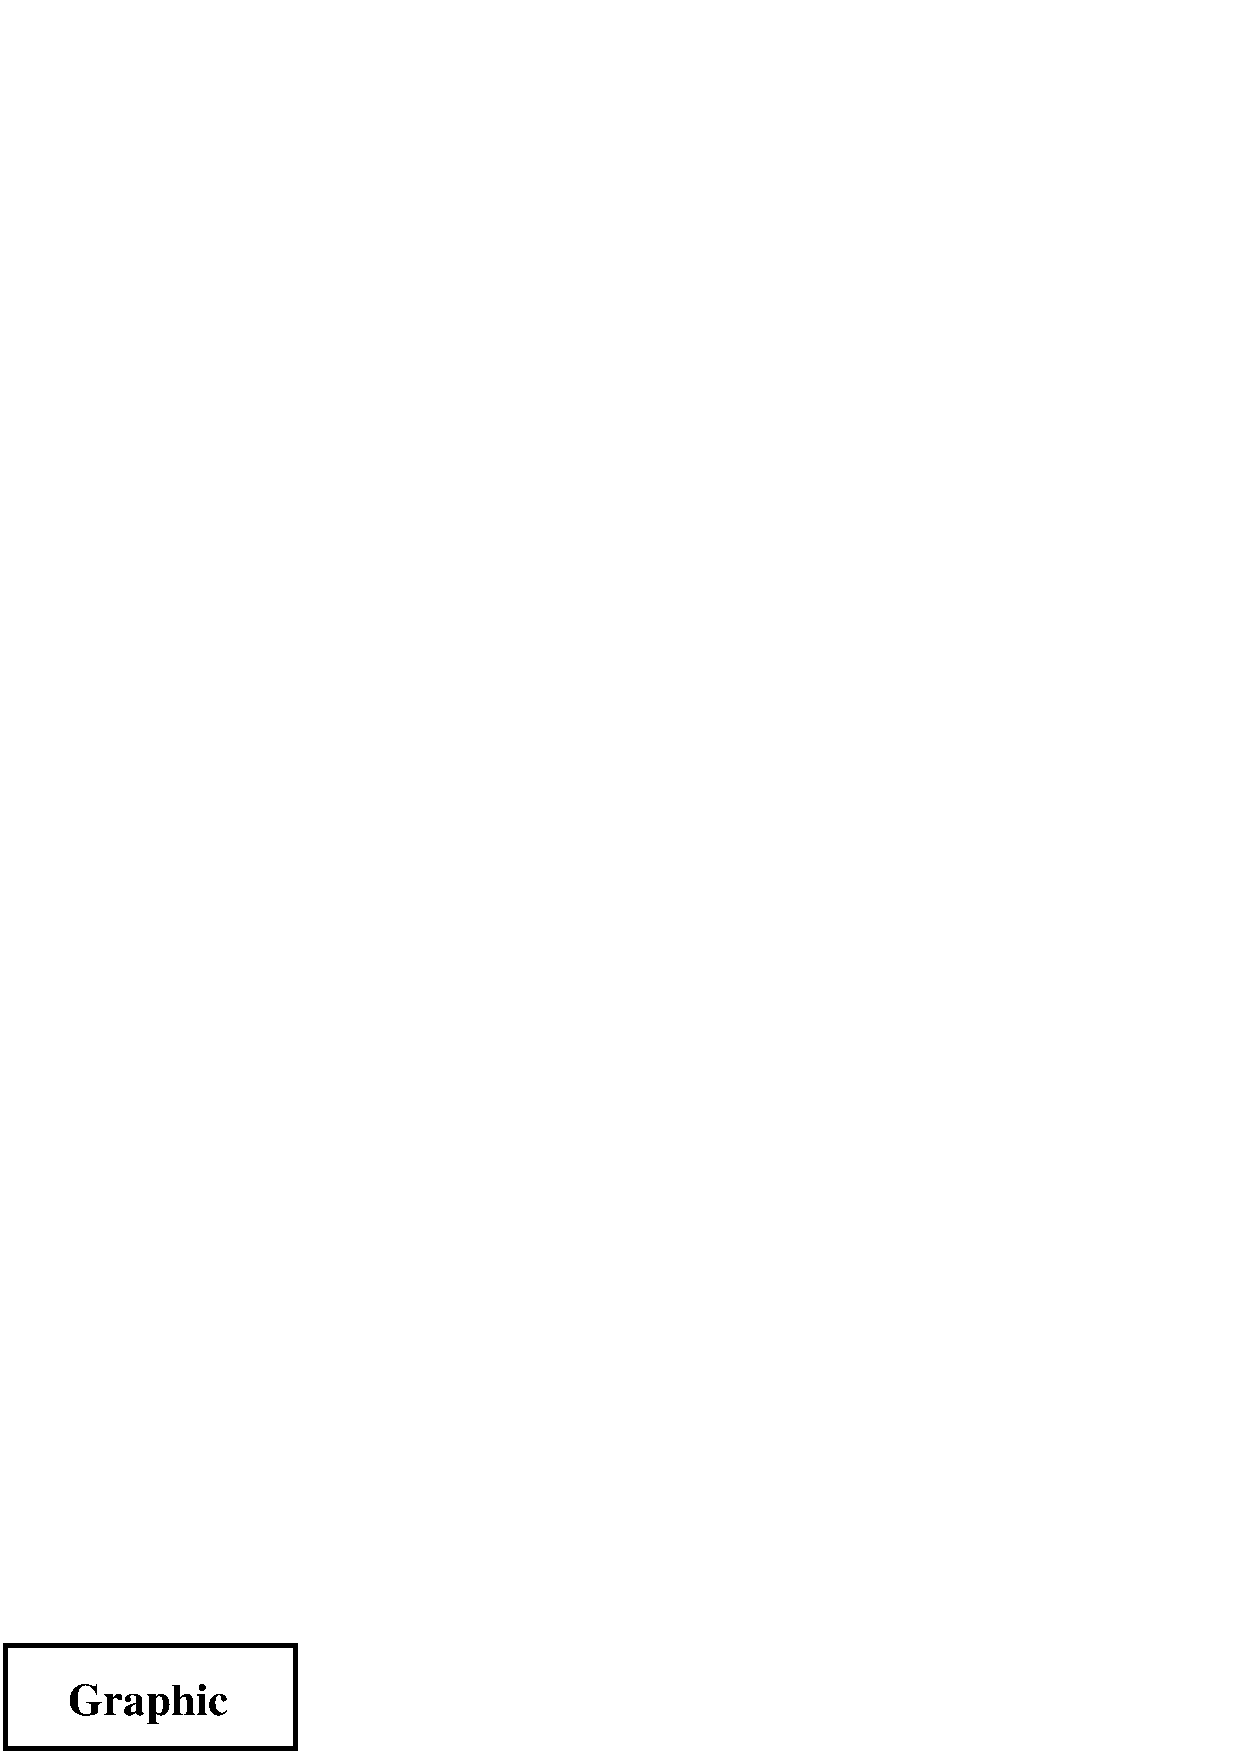
\includegraphics[width=4in]{graphic}
		\caption{Landscape Figure}
	\end{figure}
\end{landscape}
\end{lstlisting}
这是会得到一个横排的图形。
不过,由于 \env{landscape} 开始一新页,可能会导致页面出现很大空白,如同本页一样。

\begin{landscape} 
	\begin{figure} 
		\centering
		\resizebox{4in}{!}{\usebox{\boxgraphic}}
		\caption{Landscape Figure}\label{fig:landscape}
	\end{figure} 
\end{landscape}

\subsection{Sidewaysfigure 环境}\label{ssec:sidewaysfigure}

\pkgi{rotating} 宏包提供了 \envi{sidewaysfigure} 环境生成横排的图形\footnote{
	\pkg{rotating} 宏包还提供了一个 \envi{sidewaystable} 环境,
	可以生成横排的表格。}。例如:
\begin{lstlisting}
\begin{sidewaysfigure}
	\centering
	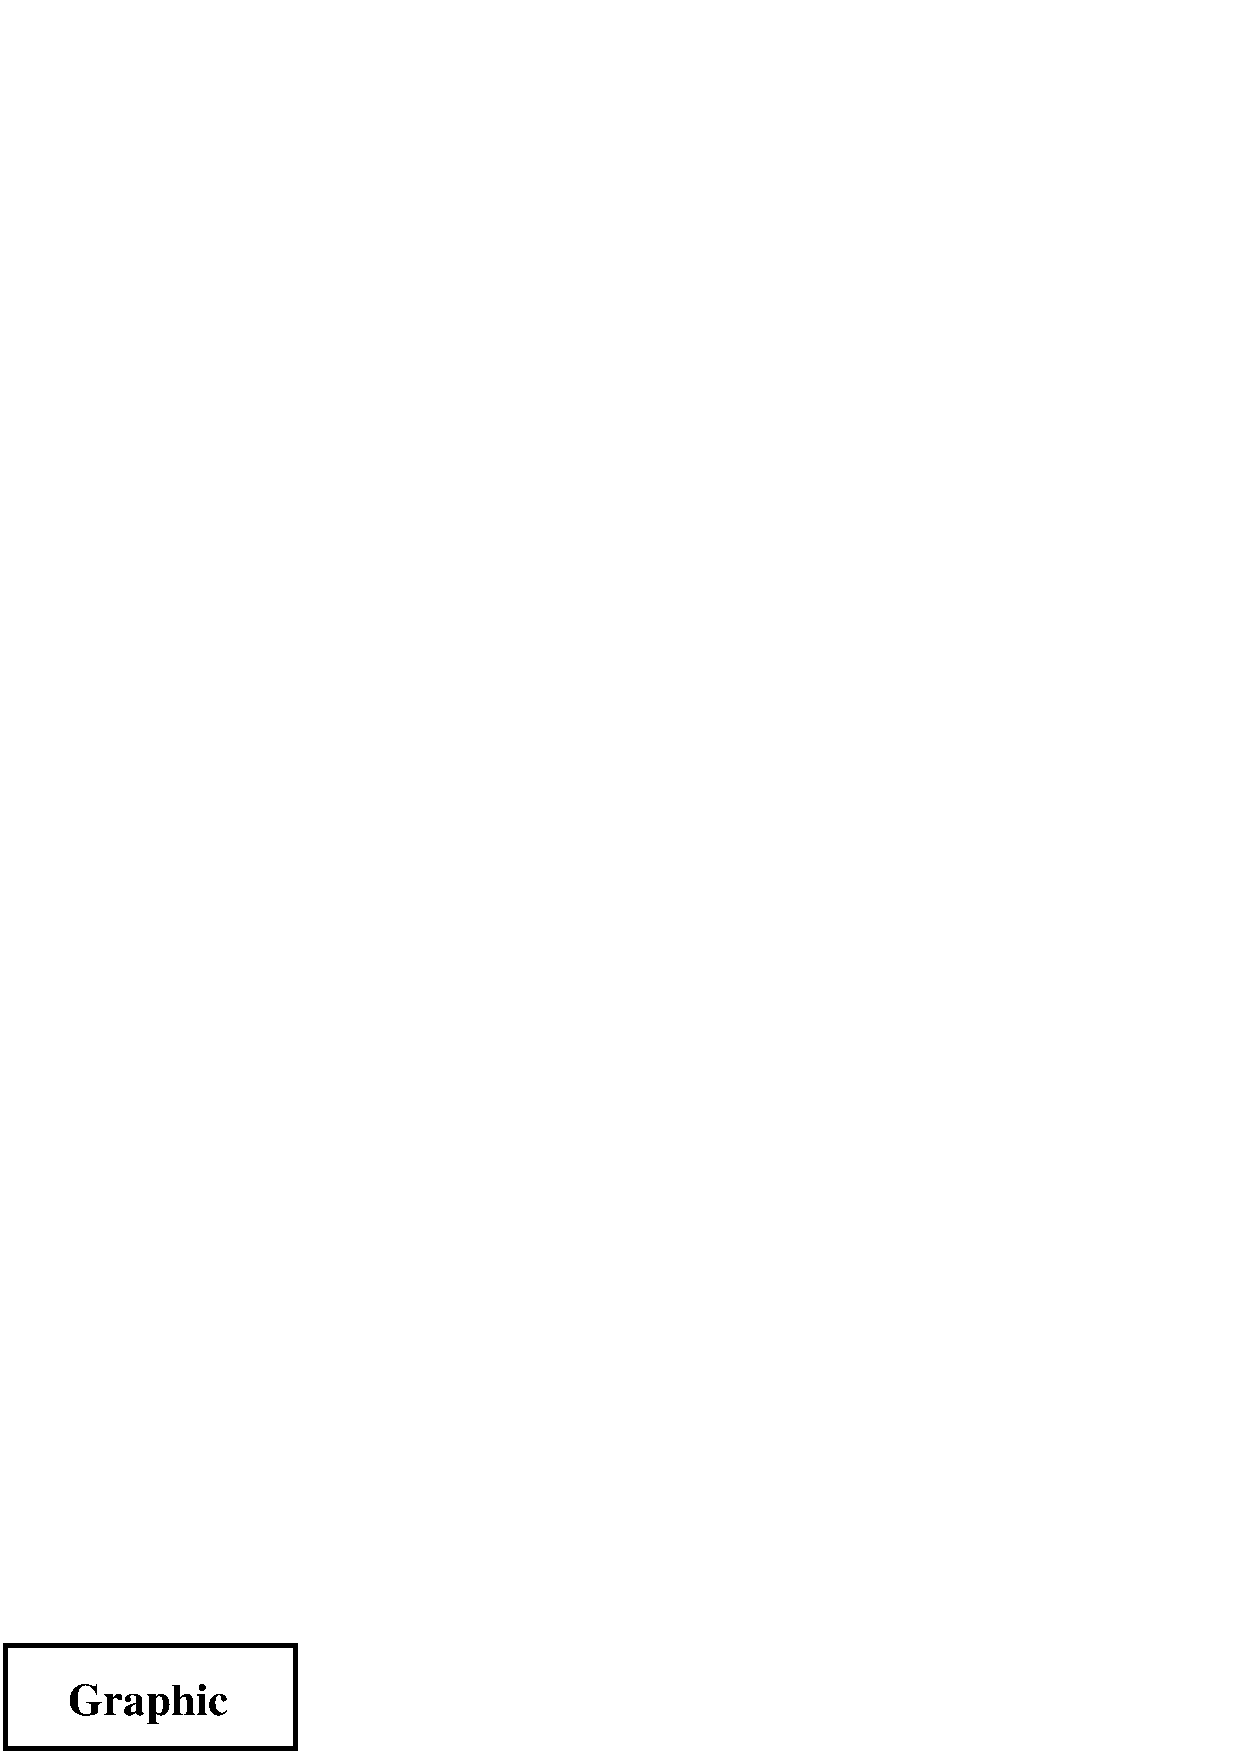
\includegraphics[width=4in]{graphic}
	\caption{Sidewaysfigure Figure}
\end{sidewaysfigure}
\end{lstlisting}
得到图~\ref{fig:sidewaysfigure}。

\begin{sidewaysfigure}
	\centering
	\resizebox{4in}{!}{\usebox{\boxgraphic}}
	\caption{Sidewaysfigure Figure}\label{fig:sidewaysfigure}
\end{sidewaysfigure}

与 \env{landscape} 环境不同的是,
由 \env{sidewaysfigure} 得到的图形可在竖排页中浮动,
从而避免导致出现过多空白的页面。
不过 \env{landscape} 环境则有更大的灵活性,允许横排页中有文本,表格和图形等。

\env{sidewaysfigure} 生成图形的默认方向取决于该文档使用 \opt{oneside} 还是 \opt{twoside} 文档类选项。
\begin{itemize}
	\item 当使用 \opt{oneside} 时,图形的底部面向竖排页的右边。
	\item 当使用 \opt{twoside} 时,图形的底部面向竖排页的外边界。
\end{itemize}
使用 \pkg{rotating} 的宏包选项可以覆盖默认设置。例如:
\begin{lstlisting}
\usepackage[figuresleft]{rotating}
\end{lstlisting}
使得用 \env{sidewaysfigure} 图像的底部位于竖排页的左边
(无论是 \opt{oneside} 还是 \opt{twoside})。同样地,
\begin{lstlisting}
\usepackage[figuresright]{rotating}
\end{lstlisting}
使得用 \env{sidewaysfigure} 图像的底部面向竖排页的右边界。

\subsection{Rotcaption 命令}

用第~\ref{ssec:landscape} 节和第~\ref{ssec:sidewaysfigure} 节的方法得到的横排图形都是放在一单独的横排页上的。
不过对于比较小的图形来说显然没有必要。
这种情况下,可以利用 \pkgi{rotating} 宏包中的 \cmdi{rotcaption} 来得到小的横排图形。例如:
\begin{lstlisting}
\begin{figure}
	\centering
	\begin{minipage}[c]{1in}
		\hfill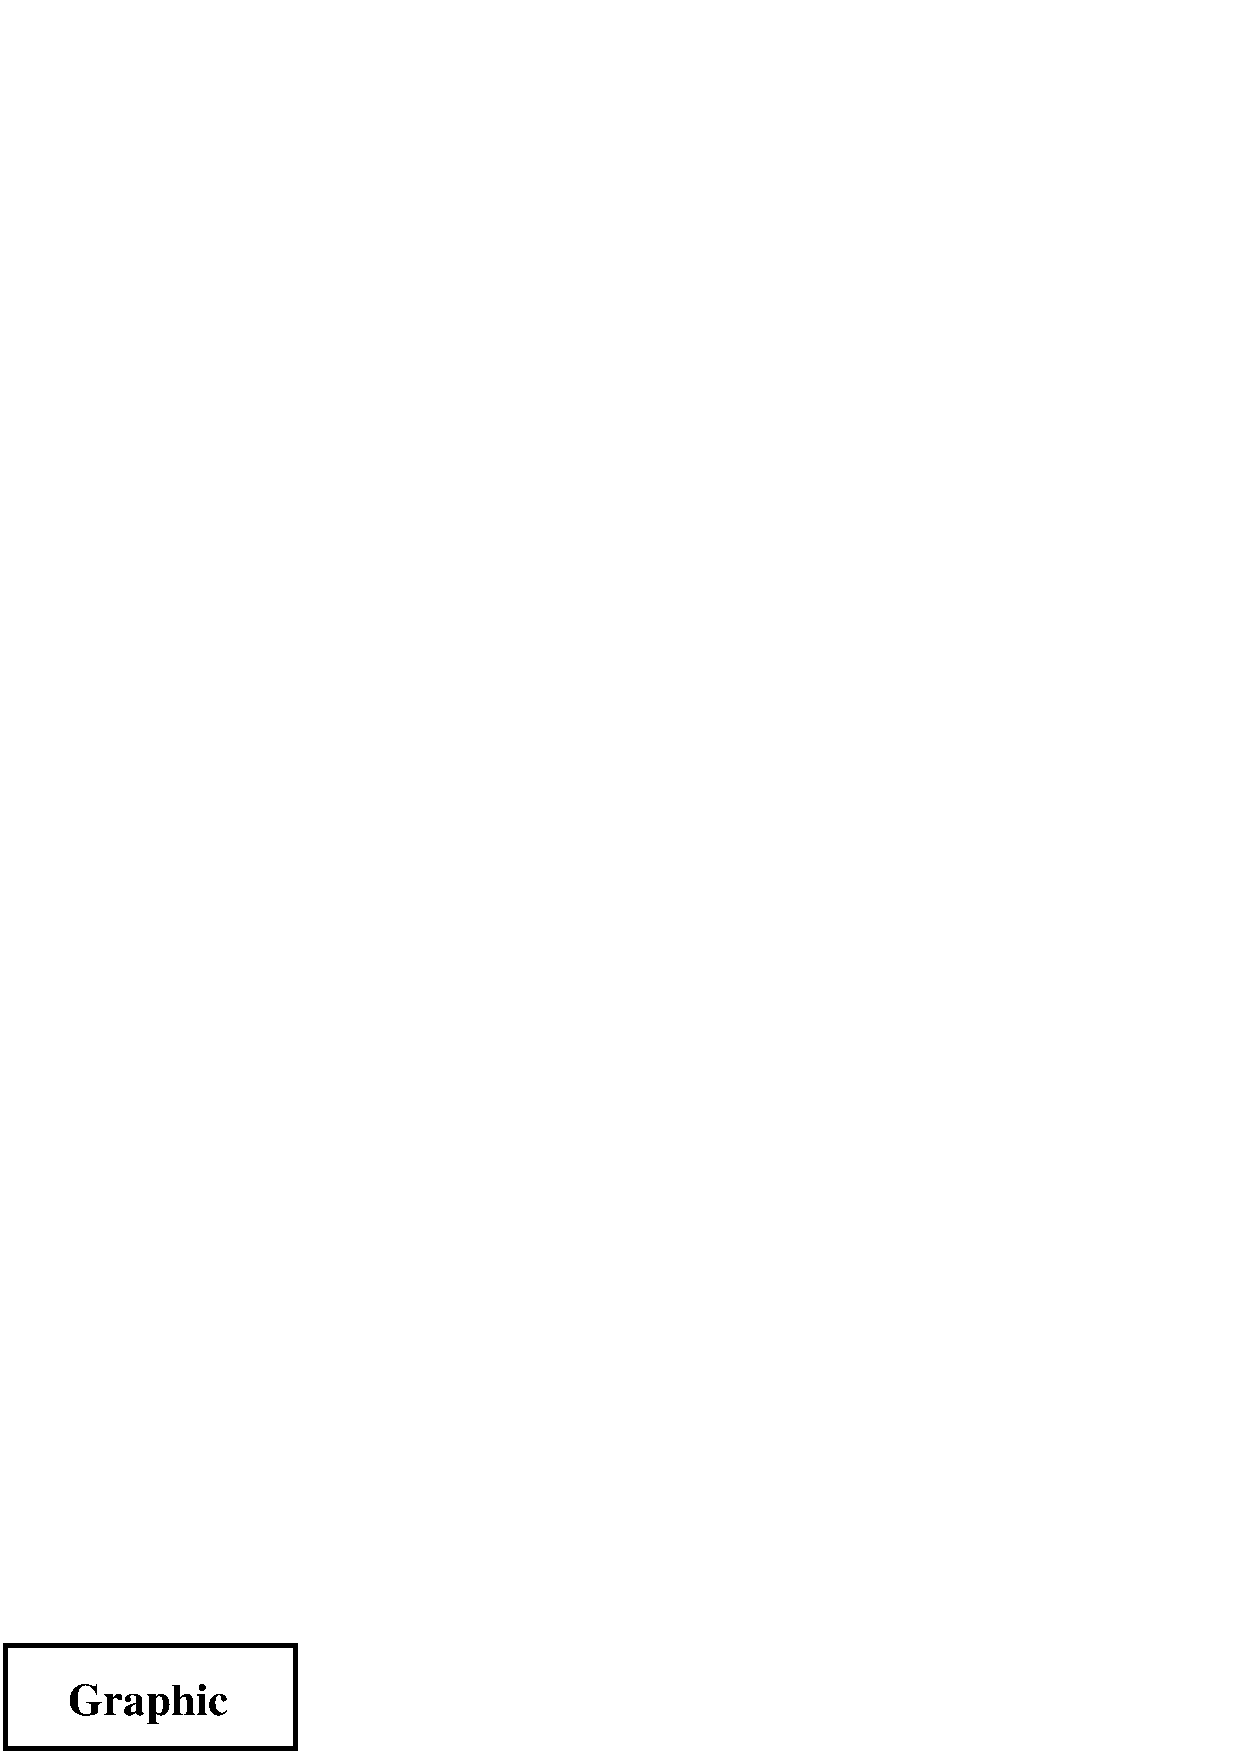
\includegraphics[width=2in,angle=90]{graphic}
	\end{minipage}%
	\hspace{0.2in}%
	\begin{minipage}[c]{0.5in}
		\captionsetup{width=2in}
		\rotcaption{由 Rotcaption 命令创建的标题}
		\label{fig:rotcaption}
	\end{minipage}
\end{figure}
\end{lstlisting}
会生成图~\ref{fig:rotcaption}。
\cmd{rotcaption} 命令生成标题的底部总是面向页面的右边界。
与第~\ref{ssec:landscape}~节和第~\ref{ssec:sidewaysfigure}~节的方法不同的是,
\cmd{rotcaption} 并不旋转图形。
因此上例中的 \cmd{includegraphics} 命令需要使用 \opt{angle=90} 这一选项。

\begin{figure}
	\centering
	\begin{minipage}[c]{1in}
		\hfill
		\rotatebox{90}{\resizebox{2in}{!}{\usebox{\boxgraphic}}}
	\end{minipage}%
	\hspace{0.2in}%
	\begin{minipage}[c]{0.5in}
		\captionsetup{width=2in}
		\rotcaption{由 Rotcaption 命令创建的标题}
		\label{fig:rotcaption}
	\end{minipage}
\end{figure}


\section{标题在一边的图形}\label{sec:sidecaption}

一般来说,图形的标题放置在其上方或下方。
本节将介绍怎样将标题放置在图形的一侧\footnote{
	因为 \pkg{float} 宏包定义的 \env{figure} 环境将标题固定在图形的下方,
	因此无法使用它来得到置于图形一侧的标题。
	不过,只要没有声明 \cmd{restylefloat} 命令,
	其它的 \pkg{float} 宏包的命令都可使用。}。


\subsection{Sidecap 宏包}\label{ssec:sidecap}

创建一侧标题最简单的途径就是使用 \pkgi{sidecap} 宏包。
该宏包定义了 \envi{SCfigure} 和 \envi{SCtable} 环境。
在其中使用 \cmd{caption} 命令时,标题就会自动放在环境内容的一侧。
例如:
\begin{lstlisting}
\usepackage{sidecap}
...
\begin{SCfigure}
	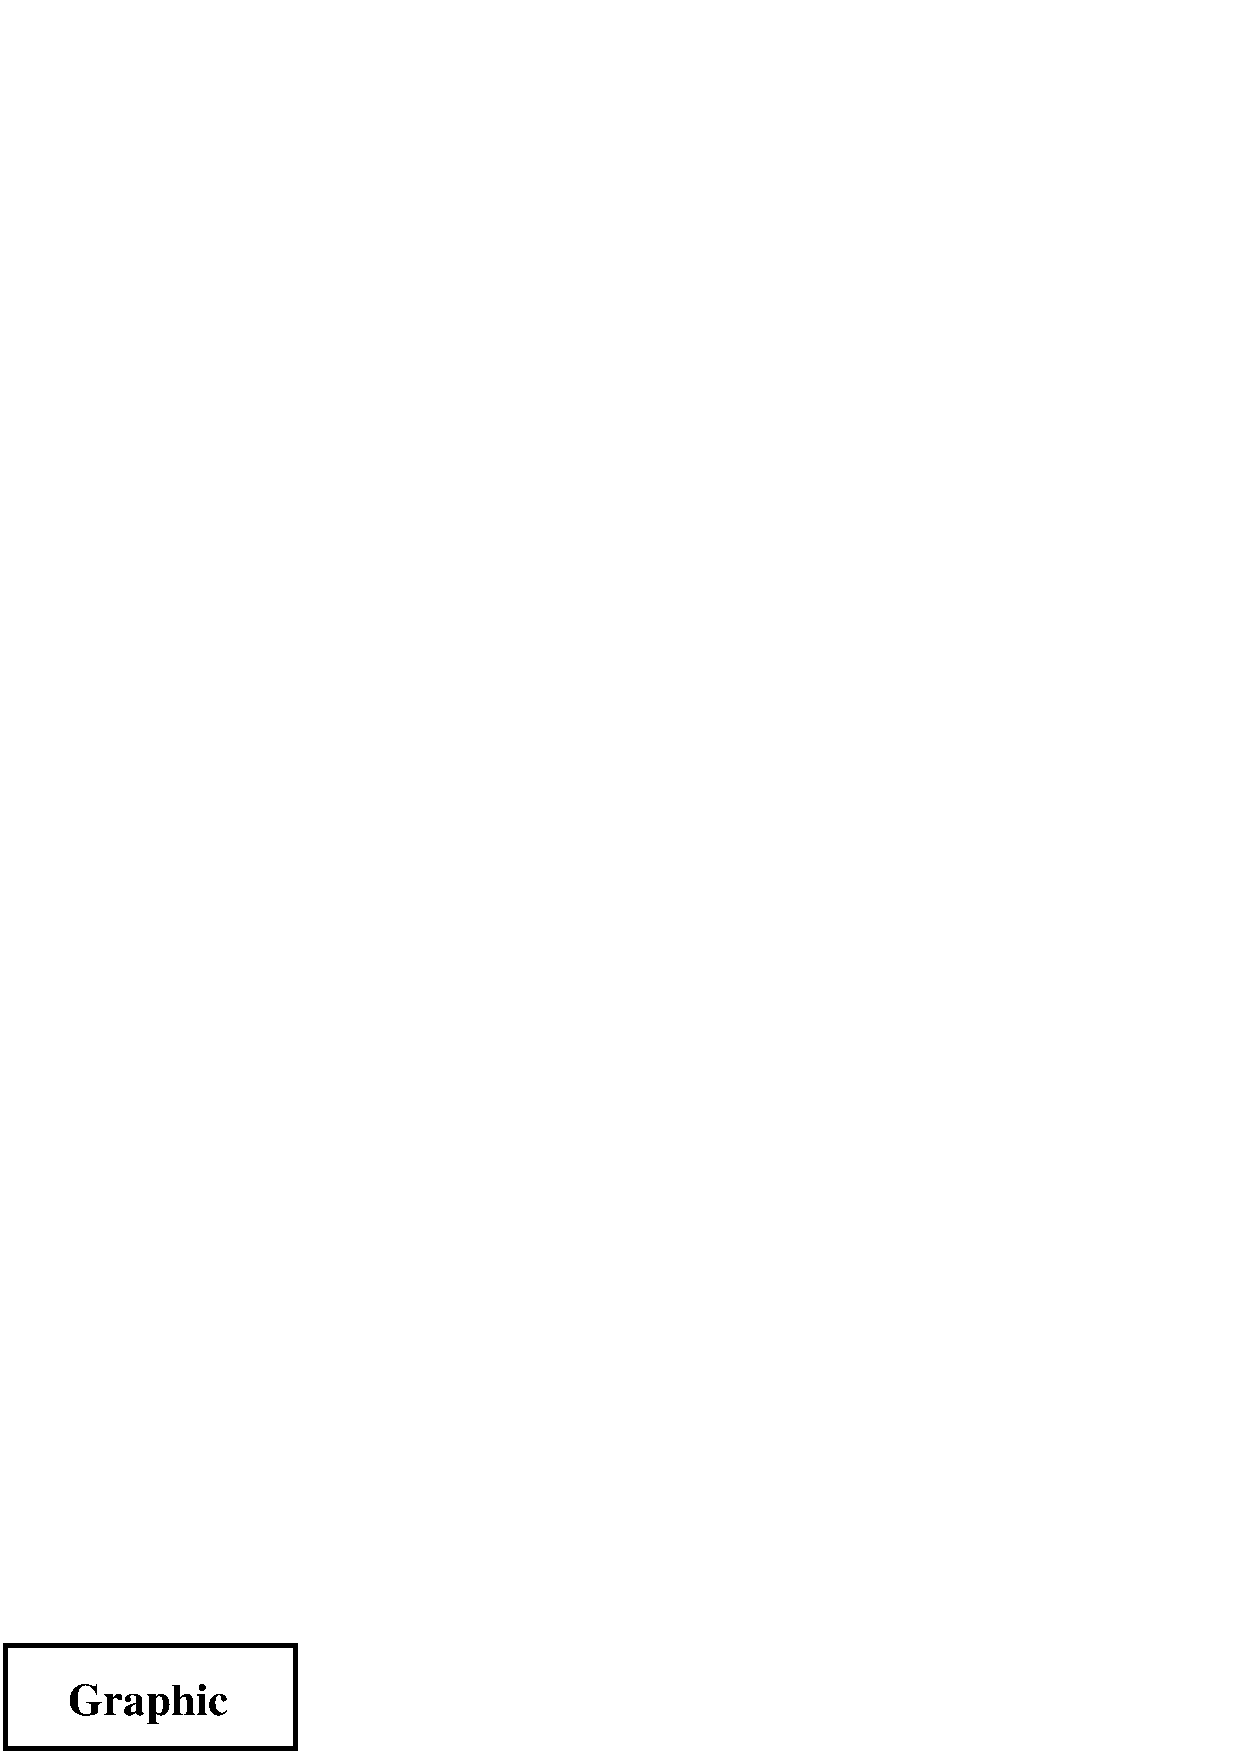
\includegraphics[width=3in]{graphic}
	\caption{This is a SCfigure}
\end{SCfigure}
\end{lstlisting}
会生成图~\ref{fig:sidecap}。

\begin{SCfigure} 
	\resizebox{3in}{!}{\usebox{\boxgraphic}}
	\caption{This is a SCfigure}
	\label{fig:sidecap}
\end{SCfigure}

\pkg{sidecap} 宏包在用 \cmd{usepackage} 调入时有下面四个可选项:
\begin{description}
	\item [outercaption] 标题在偶数页中出现在左侧,奇数页中出现在右侧。
	这也是 \pkg{sidecap} 宏包的缺省选项。
	\item [innercaption] 标题在偶数页中出现在右侧,奇数页中出现在左侧。
	\item [leftcaption]  标题总出现在左侧。
	\item [rightcaption] 标题总出现在右侧。
\end{description}

\env{Scfigure} 环境包括下面两个可选参数:
\begin{itemize}
	\item 第一个可选参数指定标题对于图形的相对宽度。
	比较大的值(如100)会让标题使用最大可能的宽度。缺省为1。
	\item 第二个可选参数指定图形的浮动位置选项,如 \opt{[htp]}或 \opt{[!ht]} 等,
	详见第~\ref{ssec:figplacement}~节。
\end{itemize}

\subsection{不使用 Sidecap 宏包时的一侧标题}

如果 \pkg{sidecap} 没有提供足够的灵活性,
用户还可以使用本节的方法生成位于一侧的标题。
第~\ref{sssec:leftcaption} 节展示了如何将标题放在图像的左侧。
放在图像右侧的方法也是类似的。
第~\ref{sssec:bindcaption} 节展示了对于双面版式的文档,
如何将标题置于图形内侧(奇数页中为图形的左侧,偶数页中为图形的右侧)。

\subsubsection{图形左侧标题}\label{sssec:leftcaption}

\cmd{caption}  命令一般将标题置于图形或表格的下方。
可以利用小页环境的技巧使得 \cmd{caption} 命令把标题放在图形的一侧。
例如命令:
\begin{lstlisting}
\begin{figure}
	\centering
	\begin{minipage}[c]{.45\linewidth}
		\centering
		\caption{Caption on the Side}
		\label{fig:side:caption}
	\end{minipage}%
	\begin{minipage}[c]{.45\linewidth}
		\centering
		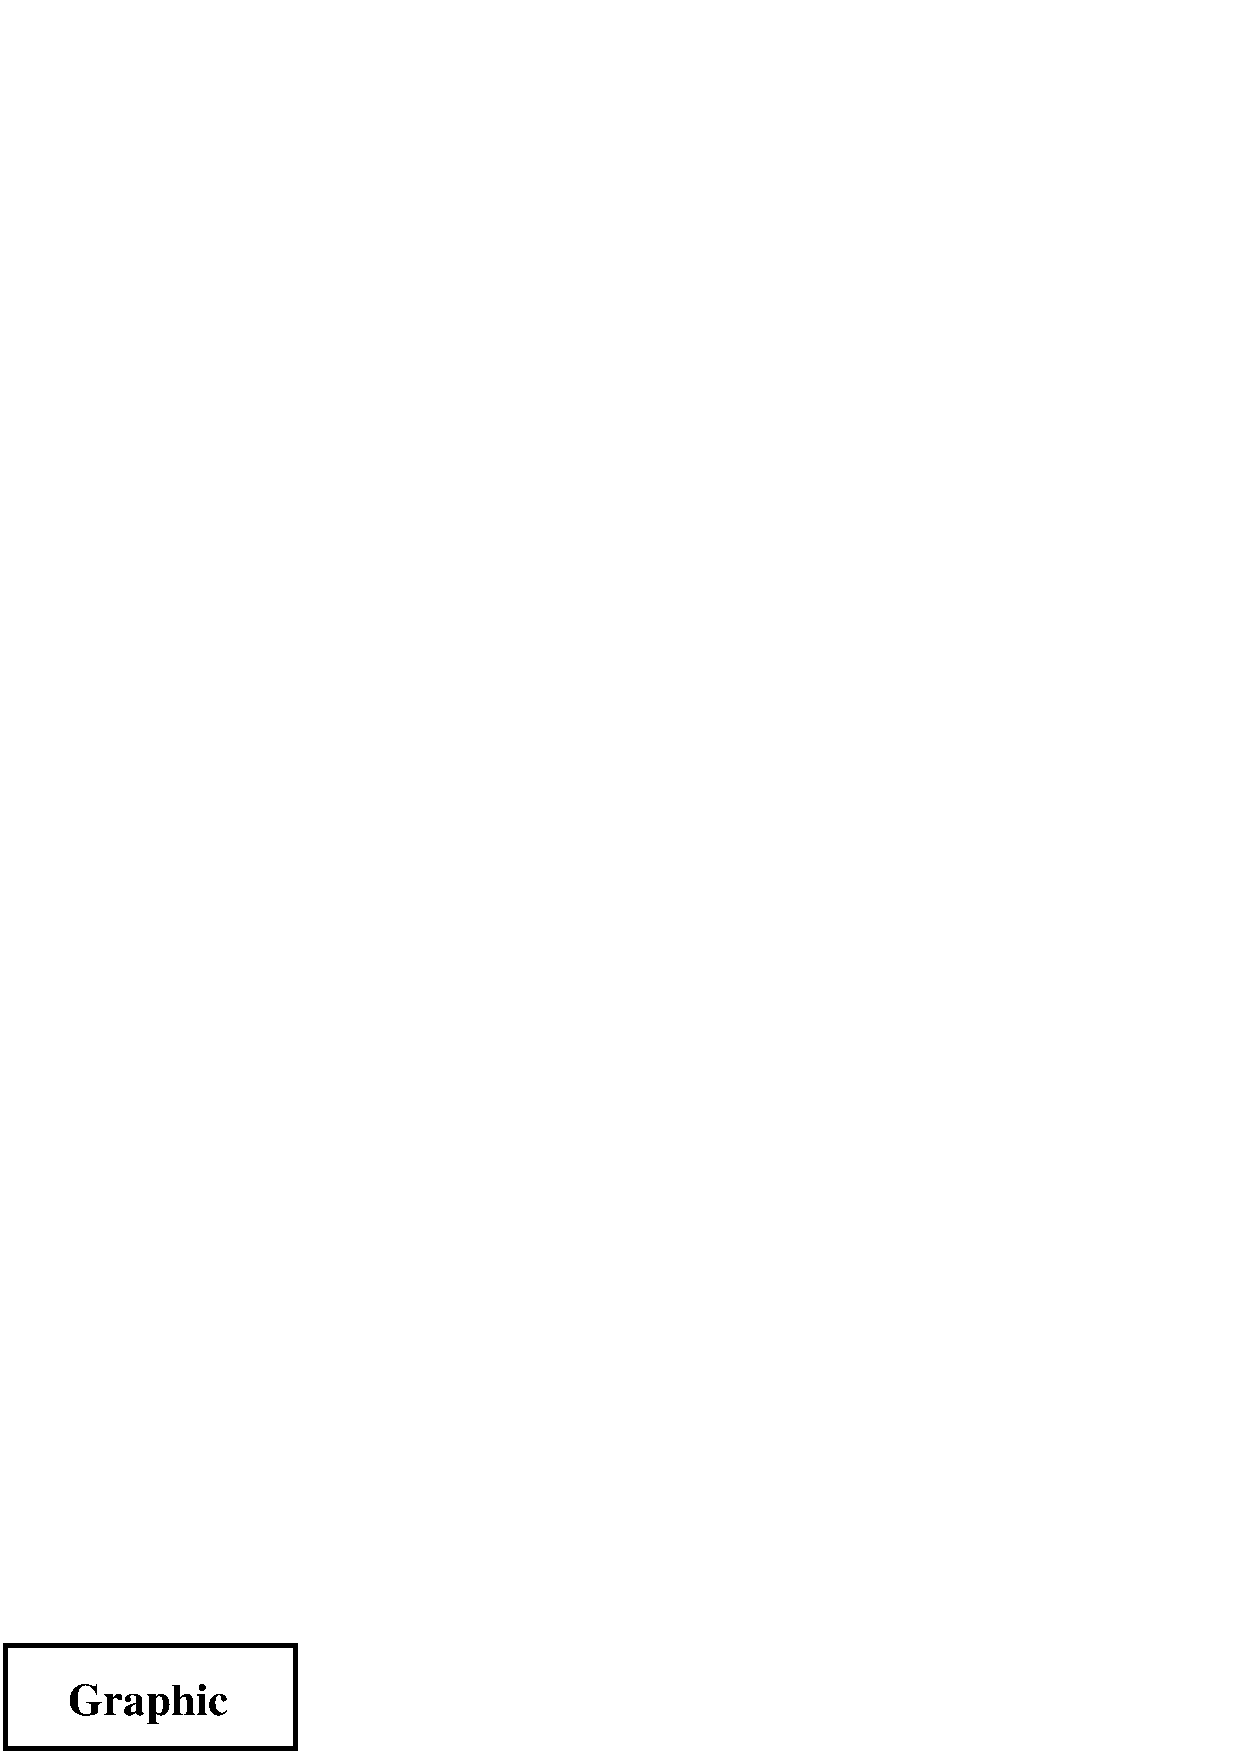
\includegraphics[width=\linewidth]{graphic}
	\end{minipage}
\end{figure}
\end{lstlisting}
得到图~\ref{fig:side:caption}。
在小页之间加入像 \cmd{hfill} 或 \cmdM{hspace}{.05\cmd{linewidth}} 的水平距离可能会更好些。

\begin{figure}
	\centering
	\begin{minipage}[c]{.45\linewidth}
		\centering
		\caption{Caption on the Side}
		\label{fig:side:caption}
	\end{minipage}%
	\begin{minipage}[c]{.45\linewidth}
		\centering
		\resizebox{\linewidth}{!}{\usebox{\boxgraphic}}
	\end{minipage}
\end{figure}

图~\ref{fig:side:caption} 中标题和图形垂直居中。
如果想让图形和标题顶部对齐或底部对齐,可参见第~\ref{ssec:minivalign}节。

\subsubsection{图形内侧标题}\label{sssec:bindcaption}

上节图~\ref{fig:side:caption}~中将标题放在图形的左侧,
而对于双面版式的文档,常常会希望将标题置于图形的内侧。
这时可用 \pkg{ifthen} 宏包的 \cmd{ifthenelse} 命令来指定对奇数页和偶数页所使用的不同代码。例如:
\begin{lstlisting}
\usepackage{ifthen}
...
\begin{figure}
	\centering
	\ifthenelse{\isodd{\pageref{fig:side:caption}}}
	{% BEGIN ODD-PAGE FIGURE
		\begin{minipage}[c]{.45\linewidth}
			\centering
			\caption{Caption on the Side}
			\label{fig:side:caption}
		\end{minipage}%
		\hspace{0.05\linewidth}%
		\begin{minipage}[c]{.45\linewidth}
			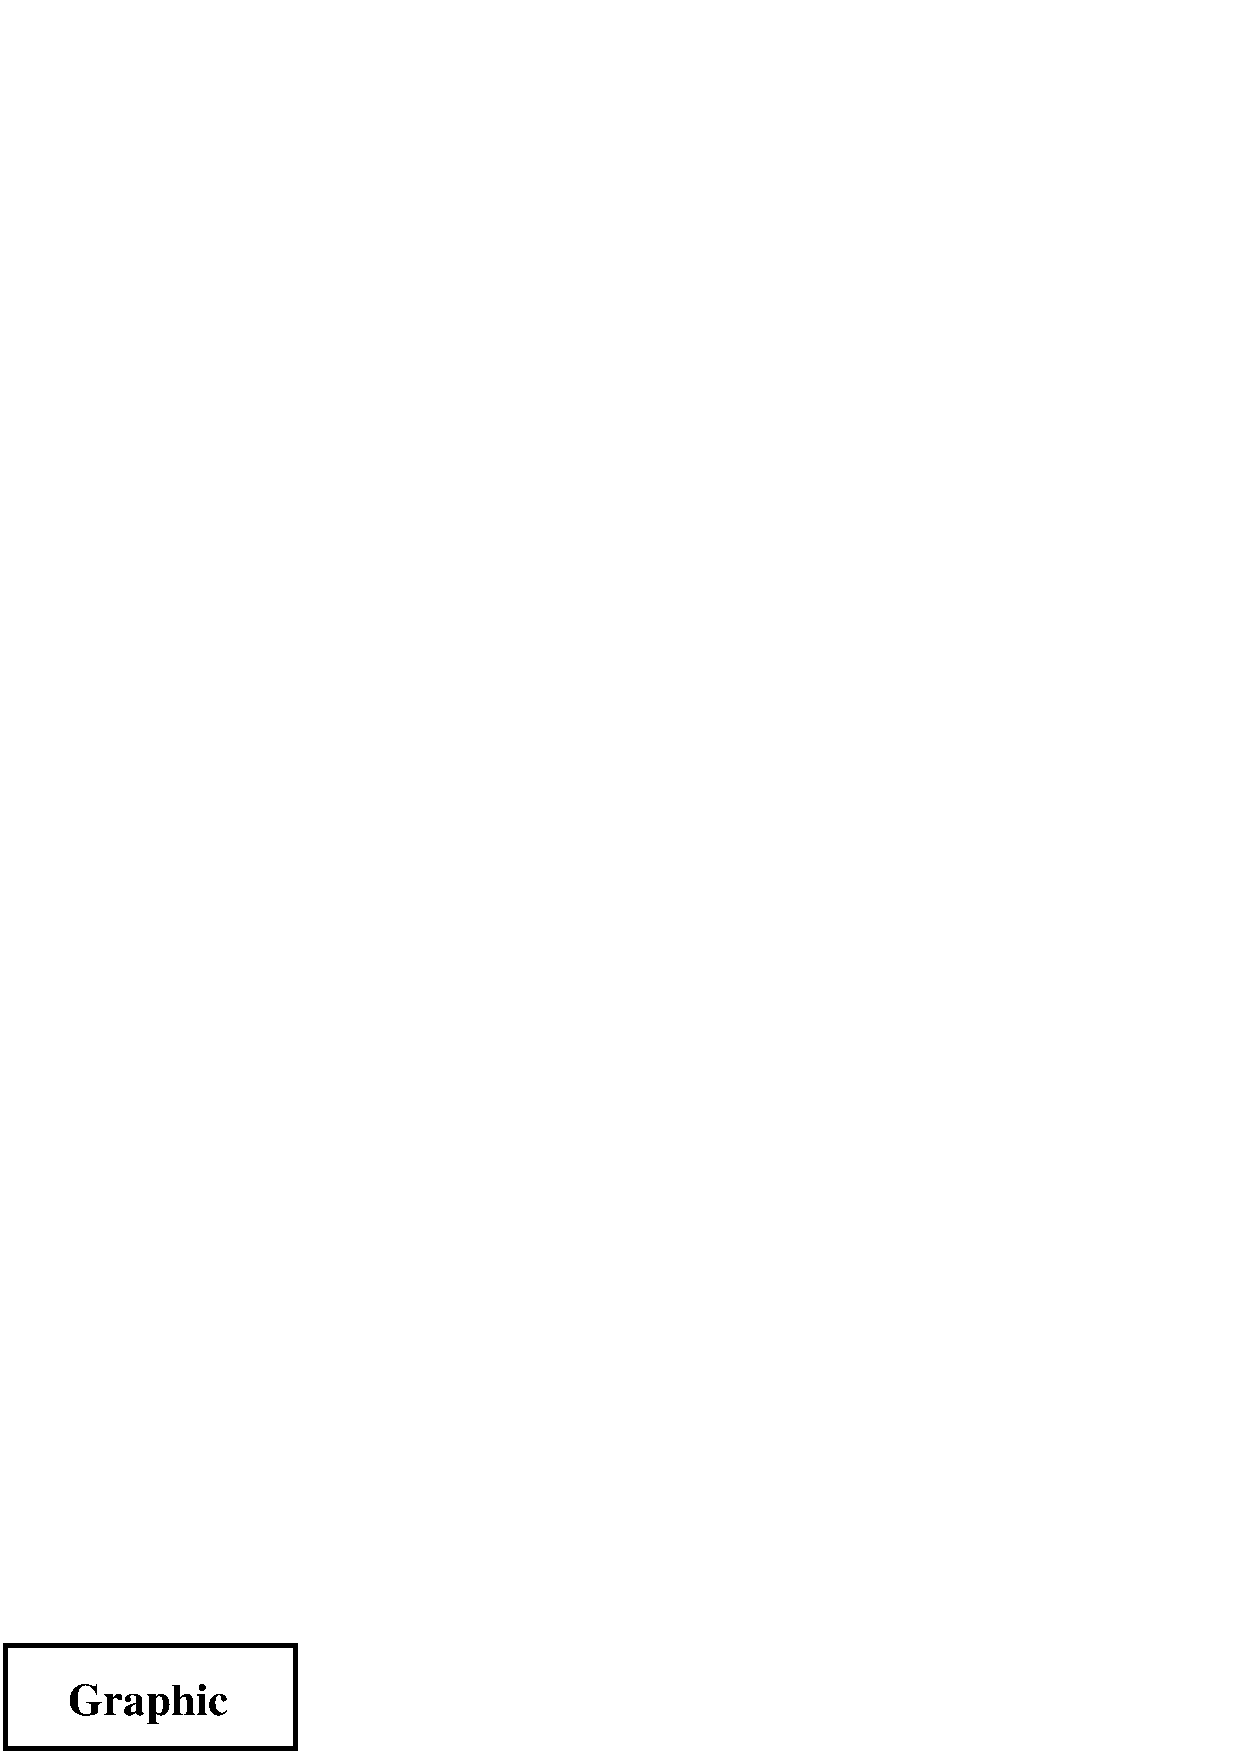
\includegraphics[width=\linewidth]{graphic}
		\end{minipage}%
	}% END ODD-PAGE FIGURE
	{% BEGIN EVEN-PAGE FIGURE
		\begin{minipage}[c]{.45\linewidth}
			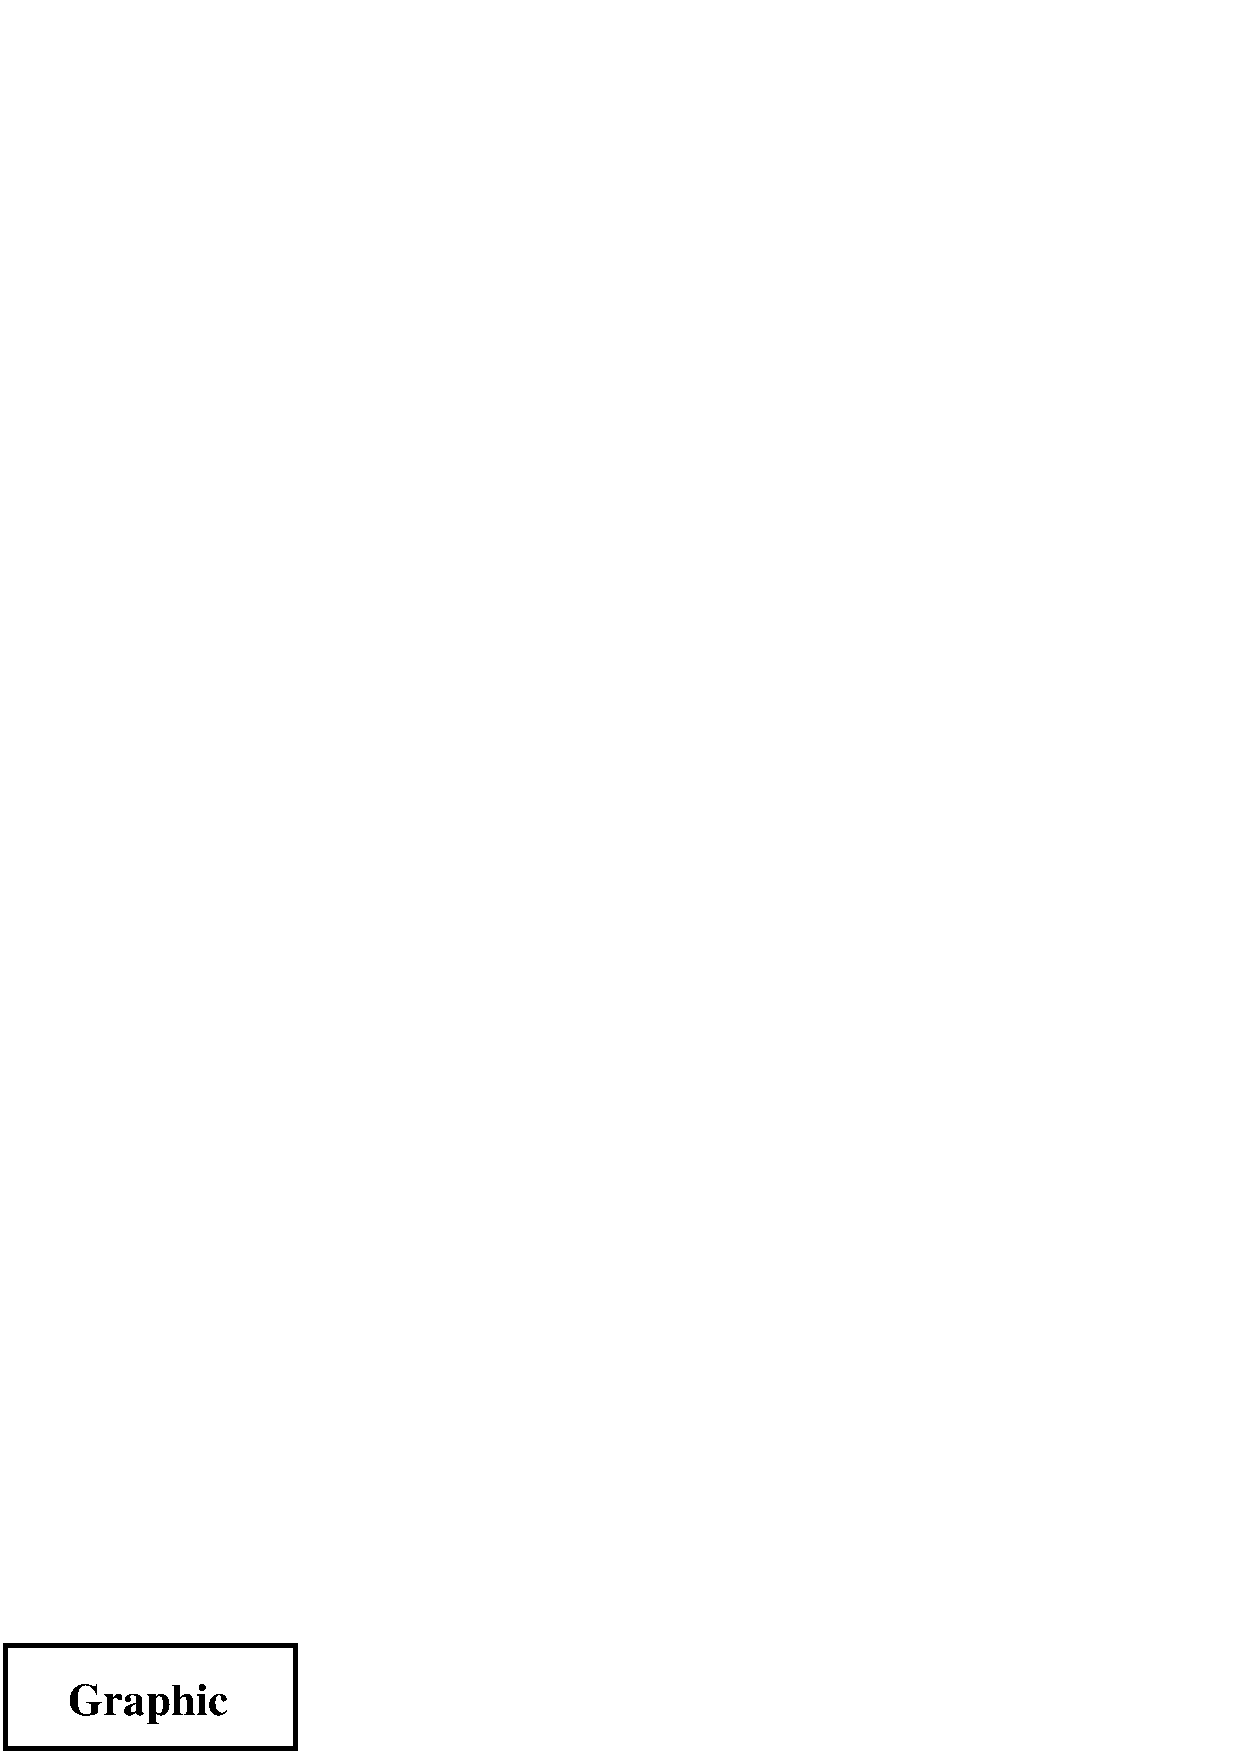
\includegraphics[width=\linewidth]{graphic}
		\end{minipage}%
		\hspace{0.05\linewidth}%
		\begin{minipage}[c]{.45\linewidth}
			\centering
			\caption{Caption on the Side}
			\label{fig:side:caption}
		\end{minipage}%
	}% END EVEN-PAGE FIGURE
\end{figure}
\end{lstlisting}
这样生成的图形其标题总在图形的内侧。


\section{奇偶页中的图形}\label{sec:evenoddpage}

图形环境的浮动放置算法不能控制图形出现在奇数页还是偶数页。
要达到控制浮动图形的奇数或偶数页放置,
必须使用 \pkgi{afterpage} 宏包的 \cmdi{afterpage} 命令和 \pkgi{ifthen} 宏包的 \cmdi{ifthenelse} 命令。

创建图形的一般方法是将图像放置于 \env{figure} 环境中。
然而,由于 \env{figure} 环境是浮动的,
因此不能保证要求放置在偶数页的图形不会浮动到奇数页(或者要求在奇数页的图形浮动到偶数页)。

不过,第~\ref{sec:nonfloat} 节介绍的 \cmd{captionof} 命令可以在不使用 \env{figure} 环境的条件下创建一个图形。
然后用 \cmd{ifthenelse} 命令将出现在奇数页上的图形放到下一偶数页上。
这需要重复使用两次插图命令,
分别对应下一页是奇数和下一页是偶数的情形。
为了简化代码,定义 \cmd{leftfig} 命令如下:
\begin{lstlisting}
\newcommand\leftfig{%
	\vspace*{\fill}%
	\centering
	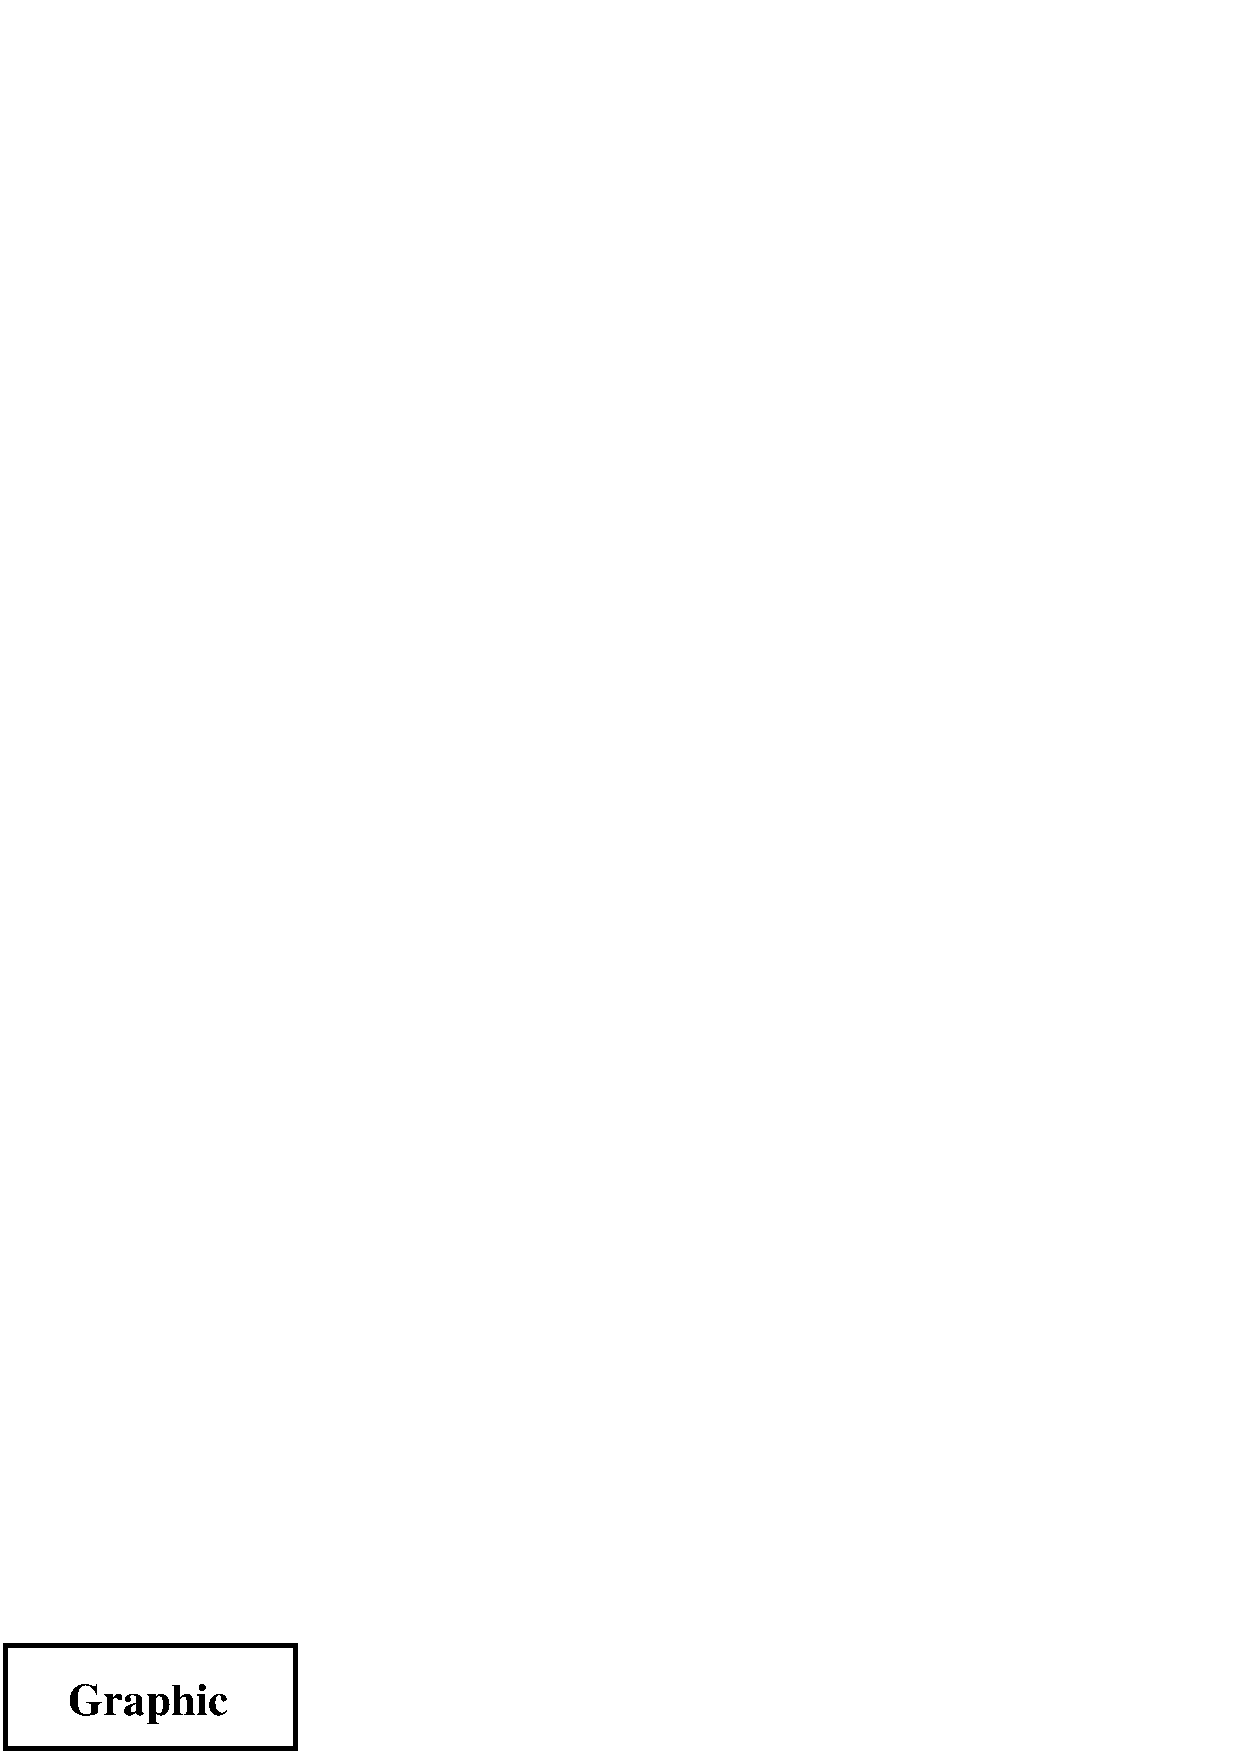
\includegraphics{graphic}
	\captionof{figure}{This is on the left (even) page.}
	\vspace*{\fill}\newpage}
\end{lstlisting}

接下来使用这个新定义的命令以及 \cmd{afterpage}、\cmd{ifthenelse} 就可以生成一幅只出现左页上的图形:
\begin{lstlisting}
\afterpage{\clearpage% 
	\ifthenelse{\isodd{\value{page}}}% 
	{\afterpage{\leftfig}}% 
	{\leftfig}}
\end{lstlisting}

关于奇偶页插图的几点说明:
\begin{itemize}
	\item 欲使图形只出现在右页(奇数页)上,掉换一下 \cmd{ifthenelse} 的参数顺序即可。
\begin{lstlisting}
\afterpage{\clearpage% 
	\ifthenelse{\isodd{\value{page}}}% 
	{\leftfig}}%
{\afterpage{\leftfig}}
\end{lstlisting}
	\item 由于这些图形是非浮动的,因此可以用 \cmdM{value}{page} 命令确定当前页码。
	注意,\cmdM{value}{page} 对于浮动图形用处不大,
	因为它指的是图形处理时的页码,不是图形放置的页码。
	因此,使用 \cmdM{value}{page} 比 \cmd{pageref} 更好,
	因为 \cmd{pageref} 只有在 \LaTeX{} 的交叉引用收敛时才正确。
	
	\item 当图形较大时,可能会出现在图形中间(例如图形与标题之间)分页的情况。
	这时可将它放到一个小页环境中以保持它的完整性。
\begin{lstlisting}
\newcommand\leftfig{%
	\vspace*{\fill}%
	\begin{minipage}{\linewidth}
		\centering
		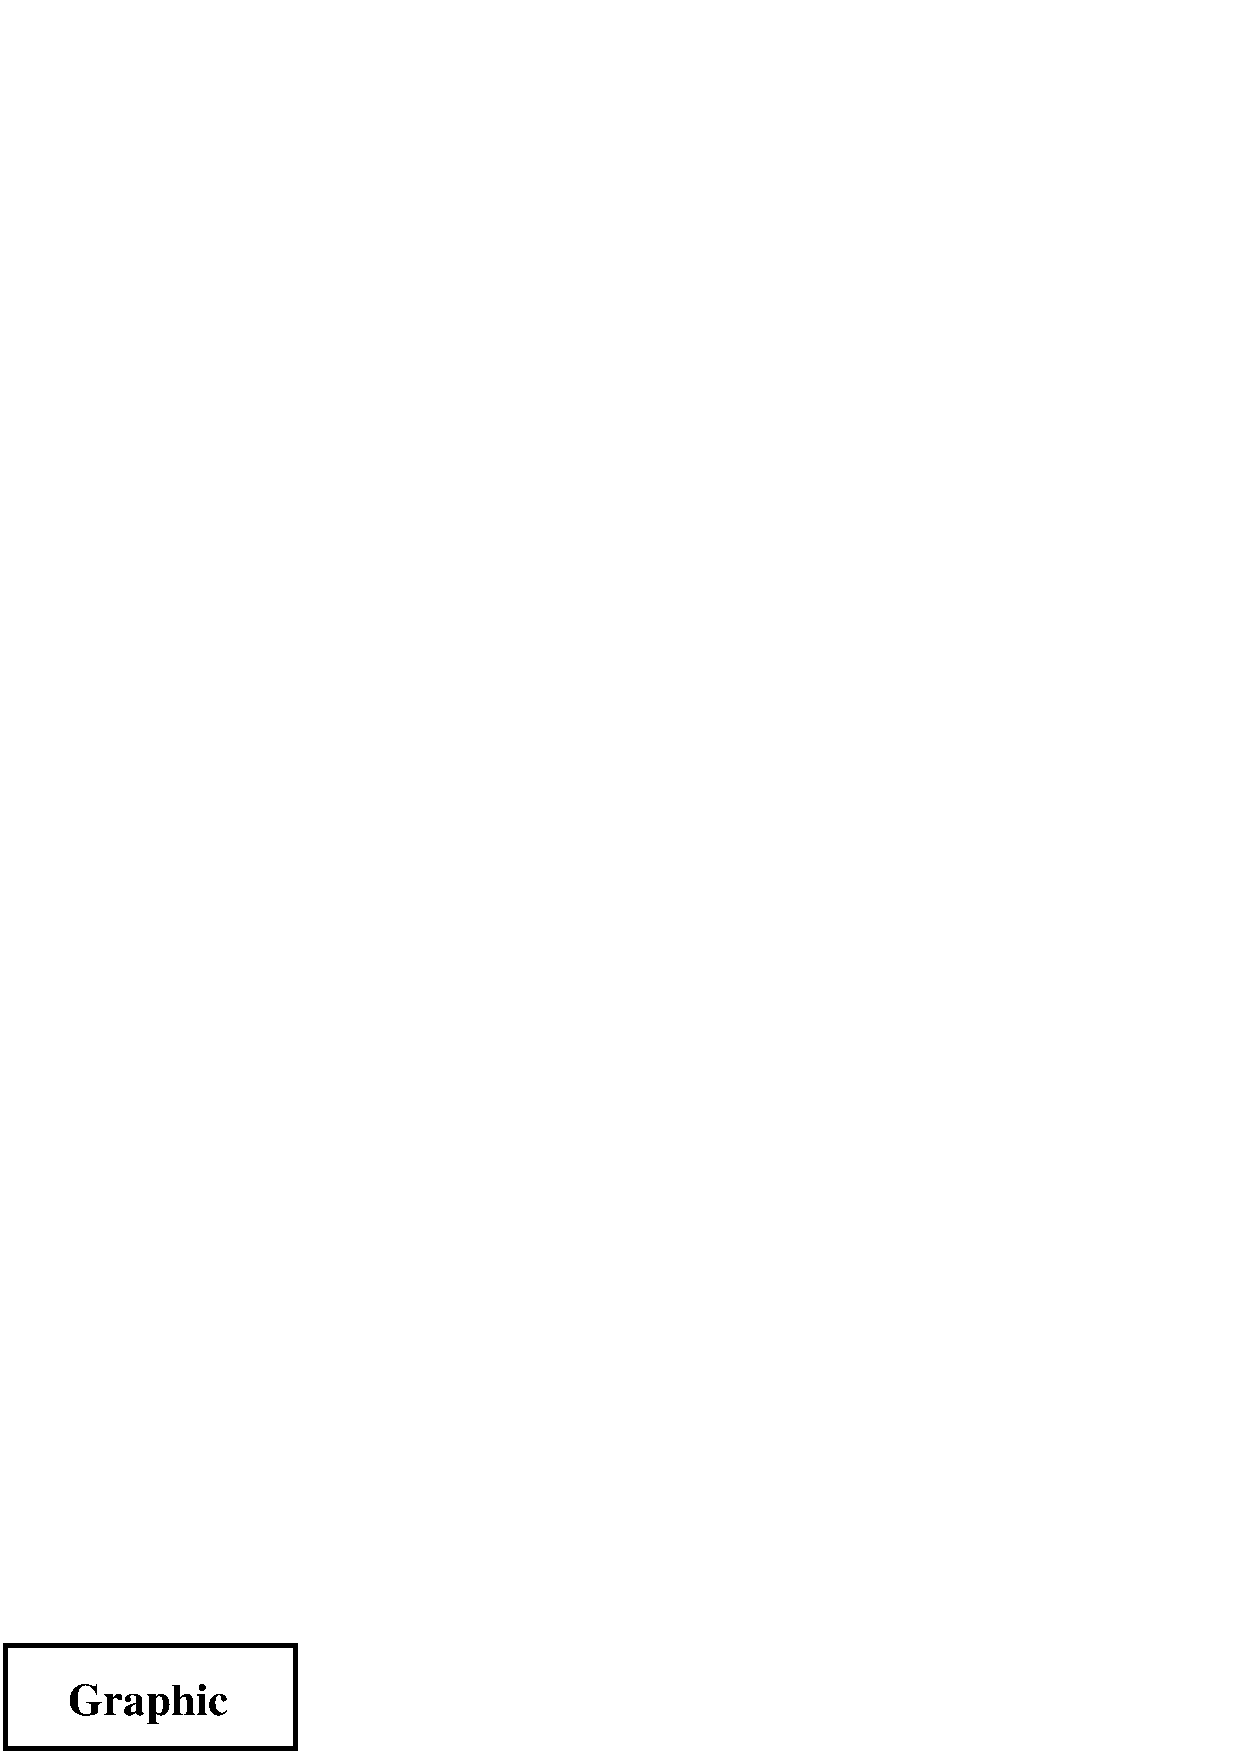
\includegraphics{graphic}
		\captionof{figure}{This is on the left (even) page.}
	\end{minipage}
	\vspace*{\fill}\newpage}
\end{lstlisting}

	\item \cmd{afterpage} 命令在极少数情况下会造成~``lost float'' 的错误。
	这时将 \cmd{clearpage} 从 \cmd{ifthenelse} 前去掉可能会有所帮助。
\begin{lstlisting}
\afterpage{\ifthenelse{\isodd{\value{page}}}%
	{\afterpage{\leftfig}}%
	{\leftfig}}
\end{lstlisting}
	
	\item 在上面的例子中,图形是占据完整的偶数页。
	要将其置于偶数页的顶部,修改或去掉 \cmdM{vspace*}{\cmd{fill}} 和 \cmd{newpage} 命令:
\begin{lstlisting}
\newcommand\leftfig{%
	\centering
	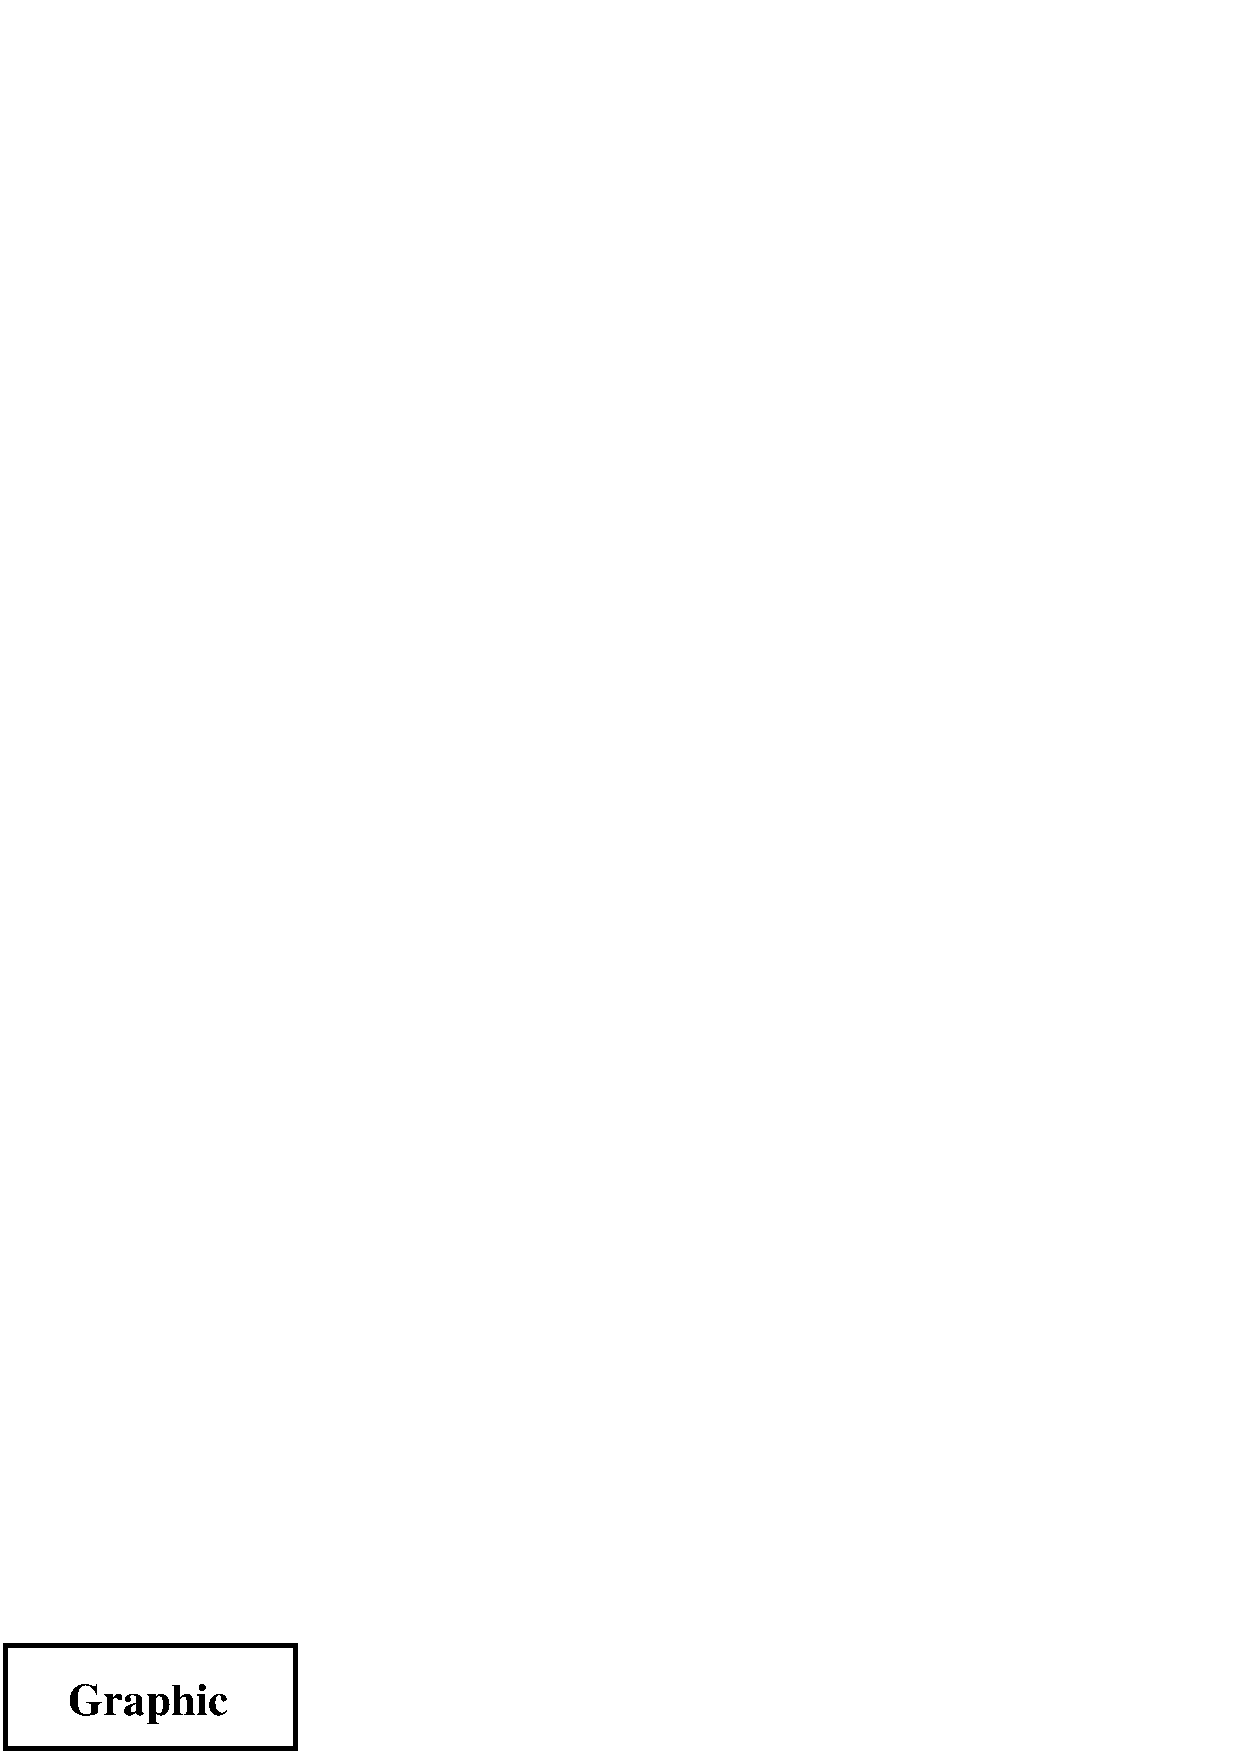
\includegraphics{graphic}
	\captionof{figure}{This is at the top of the left (even) page.}
	\vspace{\floatsep}}
\end{lstlisting}

\end{itemize}

\subsection{迎面页图形}\label{ssec:fig-facingpage}

在双面版式的文档中,为了方便图形的比较,
常常希望将两幅图形分别放在相对的迎面页(\texttt{facing page})上。
为此,需要使用类似于之前一节中放置奇偶页图形的方法。
为简单起见,定义命令 \cmd{facingfigures} 如下:
\begin{lstlisting}
\newcommand\facingfigures{%
	\vspace*{\fill}%
	\centering
	
\includegraphics{left}
	\captionof{figure}{This is on the left (even) page.}
	\vspace*{\fill}\newpage\vspace*{\fill}%
	\centering
	
\includegraphics{right}
	\captionof{figure}{This is on the right (odd) page.}
	\vspace*{\fill}\newpage}
\end{lstlisting}

这时可用 \cmd{facingfigures} 与 \cmd{afterpage}、\cmd{ifthenelse} 一起生成迎面页图形:
\begin{lstlisting}
\afterpage{\clearpage%
	\ifthenelse{\isodd{\value{page}}}%
	{\afterpage{\facingfigures}}%
	{\facingfigures}}
\end{lstlisting}


\section{盒子中的图形}\label{sec:boxfig}

盒子中的图形通常指下面两种情形:
\begin{itemize}
	\item 图形在盒子中,但其标题在盒子之外。
	\item 图形及其标题都在盒子中。
\end{itemize}

将某一对象置于盒子中的最基本的方法就是把它放到 \cmd{fbox} 命令中,
这样会将该对象用一长方形的框围起来。
\pkg{fancybox} 宏包提供了更多不同式样的盒子。


\subsection{图形在盒子中}\label{ssec:boxgraphic}

把 \cmd{includegraphics} 命令放到 \cmdi{fbox} 中会使所插入的图形置于一个带框盒子中。例如:
\begin{lstlisting}
\begin{figure}
	\centering
	\fbox{\includegraphics[totalheight=2in]{file}}
	\caption{图形在盒子中,但标题在盒子外}
	\label{fig:boxed_graphic}
\end{figure}
\end{lstlisting}
如图~\ref{fig:boxed_graphic}所示,图形被置于一带框盒子中。

\begin{figure}
	\centering
	\fbox{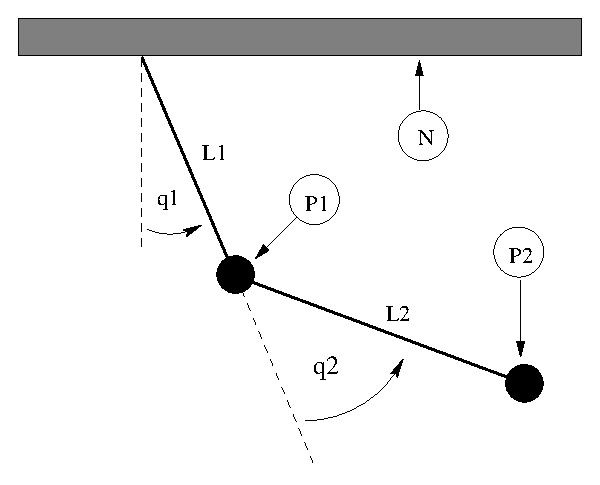
\includegraphics[totalheight=2in]{pend}}
	\caption{图形在盒子中,但标题在盒子外}
	\label{fig:boxed_graphic}
\end{figure}

\subsection{图形与标题均在盒子中}

要将图形与标题均置于盒子中,
也许有人想当然的以为把 \cmd{caption} 命令也放到 \cmd{fbox} 命中就可以了。
然而,这样做是无效的,因为 \cmd{caption} 命令只能在段落模式中使用,
而 \cmd{fbox} 命令中的内容是在左右模式中被处理\footnote{
	\LaTeX{} 使用三种模式,左右模式,段落模式和数学模式。
	参考 \cite[第36页]{Lamport1994}}。

因为小页环境和 \cmd{parbox} 命令的内容都在段落模式中处理,
所以将 \cmd{fbox} 命令的内容放到小页环境或 \cmd{parbox} 命令中,
就可以把 \cmd{caption} 包含在 \cmd{fbox} 中。
然而,由于小页环境和 \cmd{parbox} 命令都必须给出它们的宽度,
故没有直接的办法让 \cmd{fbox} 和图形及其标题一样宽。
例如下列命令:
\begin{lstlisting}
\begin{figure}
	\centering
	\fbox{ \begin{minipage}{4 in}
			\centering
			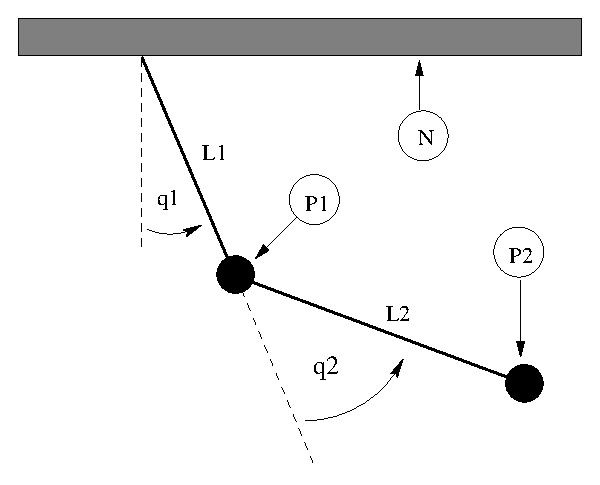
\includegraphics[totalheight=2in]{pend}
			\caption{图形和标题都在盒子中}
			\label{fig:boxed_figure}
		\end{minipage} }
\end{figure}
\end{lstlisting}
得到图~\ref{fig:boxed_figure},其中图形与标题都置于盒子中。

\begin{figure}
	\centering
	\fbox{ \begin{minipage}{4 in}
			\centering
			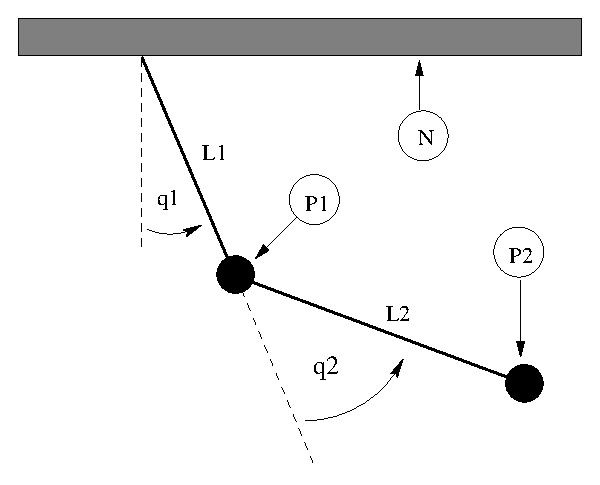
\includegraphics[totalheight=2in]{pend}
			\caption{图形和标题都在盒子中}
			\label{fig:boxed_figure}
		\end{minipage} }
	\end{figure}

一般而言,需要通过不断的尝试修改才能来确定小页环境的宽度,
从而使得盒子能够恰好围住图形和标题。
不过下面的这些方法可以避免枯燥麻烦的尝试修改。
\begin{enumerate}
	\item 任选一个确定的小页宽度,设置图形的宽度与其相同。
\begin{lstlisting}
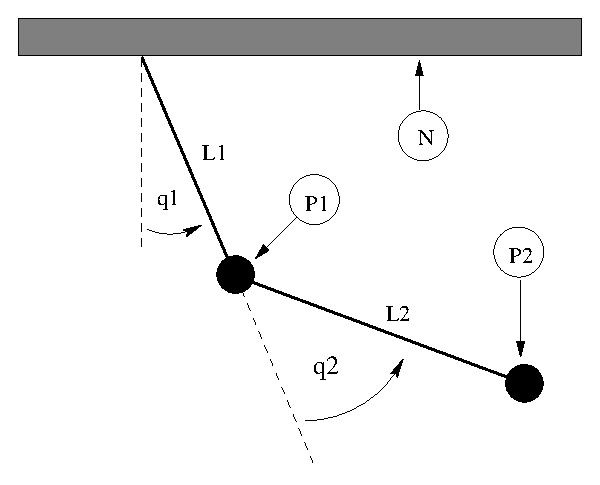
\includegraphics[width=\textwidth]{pend}
\end{lstlisting}
	\item 当指定图形的高度时,将图像放在盒子中,然后测量盒子的高度,
	即可计算出合适的小页宽度。
\begin{lstlisting}
\newsavebox{\mybox}
\newlength{\mylength}
\sbox{\mybox}{\includegraphics[height=3in]{file}}
\settowidth{\mylength}{\usebox{\mybox}}
\begin{figure}
	\centering
	\fbox{ \begin{minipage}{\mylength}
			\centering
			\usebox{\mybox}
			\caption{图形和标题都在盒子中}
			\label{fig:boxed_figure}
		\end{minipage} }
\end{figure}
\end{lstlisting}

	\item 为保证标题只有一行,
	可以使用 \cmdi{settowidth} 命令来估计标题的宽度并将其作为小页的宽度。
\begin{lstlisting}[xleftmargin=0pt]
\newlength{\mylength} 
\settowidth{\mylength}{Figure X: Box Around Figure Graphic and Caption} 
\fbox{ \begin{minipage}{\mylength} 
...
\end{lstlisting}
\end{enumerate}

\subsection{定制 fbox 的参数} \label{ssec:customizefbox}

在图~\ref{fig:boxed_graphic}~和~\ref{fig:boxed_figure}~中,
盒子的框线厚度为$0.4\pt$,在框线和图形之间有 3\pt 的空白。
可以使用 \cmd{setlength} 命令设置 \LaTeX{} 长度变量 \cmd{fboxrule} 和 \cmd{fboxsep},
进而修改这些长度。例如命令:
\begin{lstlisting}
\begin{figure}
	\centering
	\setlength{\fboxrule}{3pt}
	\setlength{\fboxsep}{1cm}
	\fbox{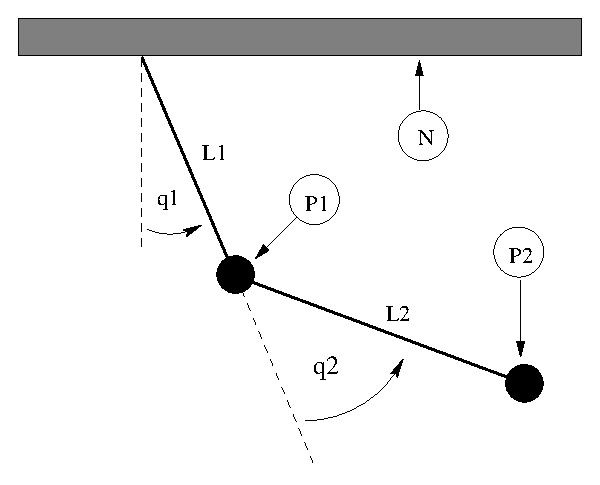
\includegraphics[totalheight=2in]{pend}}
	\caption{带有定制盒子的图形}
	\label{fig:boxed_custom}
\end{figure}
\end{lstlisting}
使得盒子的边框线厚为 3\pt 且其与图形间的距离为1厘米。
如图~\ref{fig:boxed_custom}~所示。

\begin{figure}
	\centering
	\setlength{\fboxrule}{3pt}
	\setlength{\fboxsep}{1cm}
	\fbox{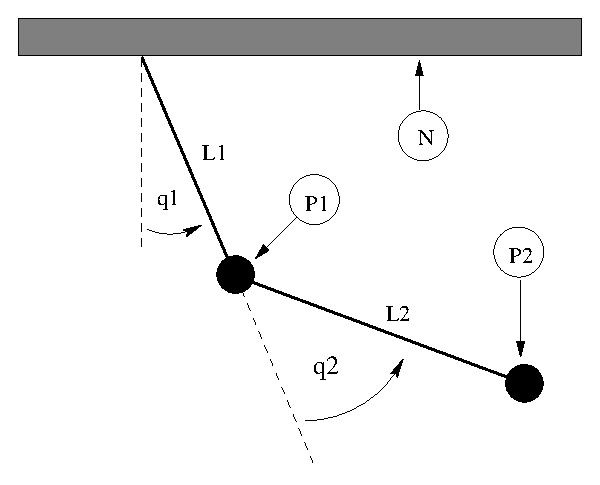
\includegraphics[totalheight=2in]{pend}}
	\caption{带有定制盒子的图形}
	\label{fig:boxed_custom}
\end{figure}


\subsection{fancybox 宏包} \label{ssec:fancybox}

在图~\ref{fig:boxed_graphic}、\ref{fig:boxed_figure}~和~\ref{fig:boxed_custom}~中,
使用 \cmd{fbox} 命令将图形包围在标准的长方形框盒子中。
要想使用不同类型的盒子,可使用 \pkgi{fancybox} 宏包。
它提供了 \cmdi{shadowbox}、\cmdi{doublebox}、\cmdi{ovalbox} 和 \cmdi{Ovalbox} 等命令来生成不同形状的盒子,如表~\ref{tab:fancyboxcmd} 所示。

\begin{table}
	\centering
	\caption{\pkg{fancybox} 命令}\label{tab:fancyboxcmd}
	\begin{tabular}{ p{0.3\textwidth} p{0.6\textwidth} }
		\toprule
		命令 & 参数  \\
		\midrule
		\begin{center}
			\cmdM{shadowbox}{Example}\\
			\shadowbox{Example}
		\end{center}  &
		\begin{itemize}
			\item 盒子边框线厚度为 \cmd{fboxrule}
			\item 盒子阴影厚度为 \cmd{shadowsize} (缺省为 $4\pt$ )。
		\end{itemize} \\
		\midrule
		\begin{center}
			\cmdM{doublebox}{Example}\\
			\doublebox{Example}
		\end{center} &
		\begin{itemize}
			\item 内框线厚为 $.75 \text{\cmd{fboxrule}}$。 
			\item 外框线厚为 $1.5 \text{\cmd{fboxrule}}$。
			\item 内外框之间的距离为 $1.5 \text{\cmd{fboxrule}} + 0.5\pt$。
		\end{itemize} \\
		\midrule
		\begin{center}
			\cmdM{ovalbox}{Example}\\
			\ovalbox{Example}
		\end{center} &
		\begin{itemize}		
			\item 盒子边框线厚度为 \cmd{thinlines}。
			\item 使用 \cmdM{cornersize}{x} 四个角的直径设为 \opt{x} 乘以盒子宽和高
			之间的较小值。\opt{x}缺省为 0.5。
			\item 使用\cmdM{cornersize*}{x} 命令直接将四个角的直径设为 \texttt{x}。
			如 \cmdM{cornersize*}{1cm} 将四个角的直径设为~1~厘米。
		\end{itemize} \\
		\midrule
		\begin{center}
			\cmdM{Ovalbox}{Example}\\
			\Ovalbox{Example}
		\end{center}  &
		除了盒子边框线厚度为 \cmd{thicklines} 外,其它均与 \cmd{ovalbox} 一样。\\
		\bottomrule
	\end{tabular}
\end{table}

如同 \cmd{fbox} 命令一样,这些盒子命令中的内容与边框间距由 \LaTeX{} 长度 \cmd{fboxsep} 控制。
与第~\ref{ssec:customizefbox} 节中的 \cmd{fboxrule} 和 \cmd{fboxsep} 相同,
长度 \cmd{shadowsize} 也可用 \cmd{setlength} 命令来设定。
而 \cmd{ovalbox} 和 \cmd{Ovalbox} 命令中的边框线厚度对应于 \env{picture} 环境中的 \cmd{thinlines} 和 \cmd{thicklines} 的值,
由于它们不是长度变量,所以无法用 \cmd{setlength} 来设定。
这两个宏的值依赖于当前字体的大小和形状,缺省分别为 $0.4\pt$ 和 $0.8\pt$。例如:
\begin{lstlisting}
\begin{figure}
	\centering
	\shadowbox{ \begin{minipage}{3.5 in}
			\centering
			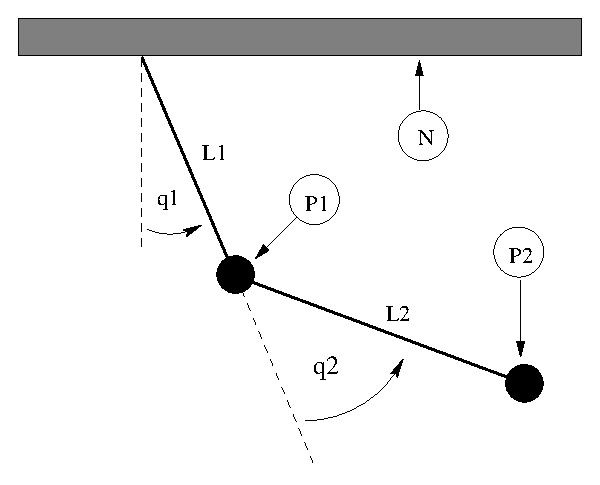
\includegraphics[totalheight=2in]{pend}
			\caption{环绕整个图形的阴影框}
			\label{fig:boxed_fancy}
	\end{minipage} }
\end{figure}
\end{lstlisting}
用一个带阴影的盒子将图形与标题包围起来,如图~\ref{fig:boxed_fancy}~所示。

\begin{figure}
	\centering
	\shadowbox{ \begin{minipage}{3.5 in}
			\centering
			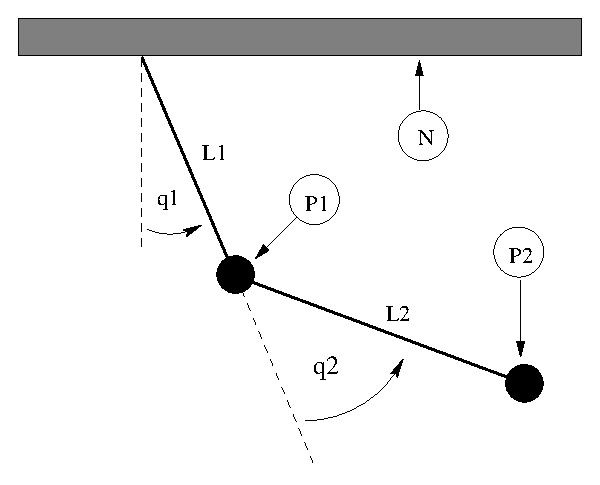
\includegraphics[totalheight=2in]{pend}
			\caption{环绕整个图形的阴影框}
			\label{fig:boxed_fancy}
	\end{minipage} }
\end{figure}


\endinput